%%%%%%%%%%%%%%%%%%%%%%%%%%%%%%%%%%%%%%%%%
% Lachaise Assignment
% LaTeX Template
% Version 1.0 (26/6/2018)
%
% This template originates from:
% http://www.LaTeXTemplates.com
%
% Authors:
% Marion Lachaise & François Févotte
% Vel (vel@LaTeXTemplates.com)
%
% License:
% CC BY-NC-SA 3.0 (http://creativecommons.org/licenses/by-nc-sa/3.0/)
% 
%%%%%%%%%%%%%%%%%%%%%%%%%%%%%%%%%%%%%%%%%

%----------------------------------------------------------------------------------------
%	PACKAGES AND OTHER DOCUMENT CONFIGURATIONS
%----------------------------------------------------------------------------------------

\documentclass{article}
\usepackage{mathtools}
\usepackage{physics}
\usepackage{amsmath}
\usepackage{setspace}
\usepackage[scale=1,bmargin=1.5cm,footnotesep=1.5cm]{geometry} %footnote spacing
\usepackage{float}
\usepackage{subcaption} %allows us to nest figures
%Using images
\usepackage{graphicx}
\graphicspath{{../images/}}

\usepackage{hyperref} %enable hyperlinks 
\hypersetup{
    colorlinks=true,
    linkcolor=violet,
    filecolor=green,      
    urlcolor=blue,
    pdftitle={Overleaf Example},
    pdfpagemode=FullScreen,
    }

% To get references:
\usepackage[nottoc,numbib]{tocbibind} % To get bibliography into table of contents
\usepackage[backend=bibtex, style=ieee]{biblatex}
\bibliography{references} 

\urlstyle{same}

%%%%%%%%%%%%%%%%%%%%%%%%%%%%%%%%%%%%%%%%%
% Lachaise Assignment
% Structure Specification File
% Version 1.0 (26/6/2018)
%
% This template originates from:
% http://www.LaTeXTemplates.com
%
% Authors:
% Marion Lachaise & François Févotte
% Vel (vel@LaTeXTemplates.com)
%
% License:
% CC BY-NC-SA 3.0 (http://creativecommons.org/licenses/by-nc-sa/3.0/)
% 
%%%%%%%%%%%%%%%%%%%%%%%%%%%%%%%%%%%%%%%%%

%----------------------------------------------------------------------------------------
%	PACKAGES AND OTHER DOCUMENT CONFIGURATIONS
%----------------------------------------------------------------------------------------

\usepackage{amsmath,amsfonts,stmaryrd,amssymb} % Math packages

\usepackage{enumerate} % Custom item numbers for enumerations

\usepackage[ruled]{algorithm2e} % Algorithms

\usepackage[framemethod=tikz]{mdframed} % Allows defining custom boxed/framed environments

\usepackage{listings} % File listings, with syntax highlighting
\lstset{
	basicstyle=\ttfamily, % Typeset listings in monospace font
}

%----------------------------------------------------------------------------------------
%	DOCUMENT MARGINS
%----------------------------------------------------------------------------------------

\usepackage{geometry} % Required for adjusting page dimensions and margins

\geometry{
	paper=a4paper, % Paper size, change to letterpaper for US letter size
	top=2.5cm, % Top margin
	bottom=3cm, % Bottom margin
	left=2.5cm, % Left margin
	right=2.5cm, % Right margin
	headheight=14pt, % Header height
	footskip=1.5cm, % Space from the bottom margin to the baseline of the footer
	headsep=1.2cm, % Space from the top margin to the baseline of the header
	%showframe, % Uncomment to show how the type block is set on the page
}

%----------------------------------------------------------------------------------------
%	FONTS
%----------------------------------------------------------------------------------------

\usepackage[utf8]{inputenc} % Required for inputting international characters
\usepackage[T1]{fontenc} % Output font encoding for international characters

\usepackage{XCharter} % Use the XCharter fonts

%----------------------------------------------------------------------------------------
%	COMMAND LINE ENVIRONMENT
%----------------------------------------------------------------------------------------

% Usage:
% \begin{commandline}
%	\begin{verbatim}
%		$ ls
%		
%		Applications	Desktop	...
%	\end{verbatim}
% \end{commandline}

\mdfdefinestyle{commandline}{
	leftmargin=10pt,
	rightmargin=10pt,
	innerleftmargin=15pt,
	middlelinecolor=black!50!white,
	middlelinewidth=2pt,
	frametitlerule=false,
	backgroundcolor=black!5!white,
	frametitle={Command Line},
	frametitlefont={\normalfont\sffamily\color{white}\hspace{-1em}},
	frametitlebackgroundcolor=black!50!white,
	nobreak,
}

% Define a custom environment for command-line snapshots
\newenvironment{commandline}{
	\medskip
	\begin{mdframed}[style=commandline]
}{
	\end{mdframed}
	\medskip
}

%----------------------------------------------------------------------------------------
%	FILE CONTENTS ENVIRONMENT
%----------------------------------------------------------------------------------------

% Usage:
% \begin{file}[optional filename, defaults to "File"]
%	File contents, for example, with a listings environment
% \end{file}

\mdfdefinestyle{file}{
	innertopmargin=1.6\baselineskip,
	innerbottommargin=0.8\baselineskip,
	topline=false, bottomline=false,
	leftline=false, rightline=false,
	leftmargin=2cm,
	rightmargin=2cm,
	singleextra={%
		\draw[fill=black!10!white](P)++(0,-1.2em)rectangle(P-|O);
		\node[anchor=north west]
		at(P-|O){\ttfamily\mdfilename};
		%
		\def\l{3em}
		\draw(O-|P)++(-\l,0)--++(\l,\l)--(P)--(P-|O)--(O)--cycle;
		\draw(O-|P)++(-\l,0)--++(0,\l)--++(\l,0);
	},
	nobreak,
}

% Define a custom environment for file contents
\newenvironment{file}[1][File]{ % Set the default filename to "File"
	\medskip
	\newcommand{\mdfilename}{#1}
	\begin{mdframed}[style=file]
}{
	\end{mdframed}
	\medskip
}

%----------------------------------------------------------------------------------------
%	NUMBERED QUESTIONS ENVIRONMENT
%----------------------------------------------------------------------------------------

% Usage:
% \begin{question}[optional title]
%	Question contents
% \end{question}

\mdfdefinestyle{question}{
	innertopmargin=1.2\baselineskip,
	innerbottommargin=0.8\baselineskip,
	roundcorner=5pt,
	nobreak,
	singleextra={%
		\draw(P-|O)node[xshift=1em,anchor=west,fill=white,draw,rounded corners=5pt]{%
		Question \theQuestion\questionTitle};
	},
}

\newcounter{Question} % Stores the current question number that gets iterated with each new question

% Define a custom environment for numbered questions
\newenvironment{question}[1][\unskip]{
	\bigskip
	\stepcounter{Question}
	\newcommand{\questionTitle}{~#1}
	\begin{mdframed}[style=question]
}{
	\end{mdframed}
	\medskip
}

%----------------------------------------------------------------------------------------
%	WARNING TEXT ENVIRONMENT
%----------------------------------------------------------------------------------------

% Usage:
% \begin{warn}[optional title, defaults to "Warning:"]
%	Contents
% \end{warn}

\mdfdefinestyle{warning}{
	topline=false, bottomline=false,
	leftline=false, rightline=false,
	nobreak,
	singleextra={%
		\draw(P-|O)++(-0.5em,0)node(tmp1){};
		\draw(P-|O)++(0.5em,0)node(tmp2){};
		\fill[black,rotate around={45:(P-|O)}](tmp1)rectangle(tmp2);
		\node at(P-|O){\color{white}\scriptsize\bf !};
		\draw[very thick](P-|O)++(0,-1em)--(O);%--(O-|P);
	}
}

% Define a custom environment for warning text
\newenvironment{warn}[1][Warning:]{ % Set the default warning to "Warning:"
	\medskip
	\begin{mdframed}[style=warning]
		\noindent{\textbf{#1}}
}{
	\end{mdframed}
}

%----------------------------------------------------------------------------------------
%	INFORMATION ENVIRONMENT
%----------------------------------------------------------------------------------------

% Usage:
% \begin{info}[optional title, defaults to "Info:"]
% 	contents
% 	\end{info}

\mdfdefinestyle{info}{%
	topline=false, bottomline=false,
	leftline=false, rightline=false,
	nobreak,
	singleextra={%
		\fill[black](P-|O)circle[radius=0.4em];
		\node at(P-|O){\color{white}\scriptsize\bf i};
		\draw[very thick](P-|O)++(0,-0.8em)--(O);%--(O-|P);
	}
}

% Define a custom environment for information
\newenvironment{info}[1][Info:]{ % Set the default title to "Info:"
	\medskip
	\begin{mdframed}[style=info]
		\noindent{\textbf{#1}}
}{
	\end{mdframed}
}
 % Include the file specifying the document structure and custom commands

%----------------------------------------------------------------------------------------

\begin{document}
\onehalfspacing
\parindent=0pt          %  Switch off indent of paragraphs

%----------------------------------------------------------------------------------------
%	TITLE PAGE
%----------------------------------------------------------------------------------------

\thispagestyle{empty}

\vspace*{0.1\textheight}

\begin{center}
        \huge{\bfseries Quantum Computing Project Group 5}\\
\end{center}

\bigskip

\begin{center}
        \large{Jabeth Musumba}\\
        \large{Yi Sheng Ng}\\
        \large{Finn John Onori}\\
        \large{Tiernan Stapleton}\\
        \large{Riddhi Yadav}\\
        \large{Han Yoong}\\
        \bigskip
        \large{March 23, 2022}
\end{center}

\vspace*{0.4\textheight}

\begin{center}
        
\includegraphics[width=35mm]{crest.pdf}
\end{center}

\medskip

\newpage

%----------------------------------------------------------------------------------------
%	INTRODUCTION
%----------------------------------------------------------------------------------------
\vspace{10mm}
\hrule

\vspace{10mm}

\section*{Introduction} % Unnumbered section
\vspace{10mm}

The objective of our project is to build an application which implements the Grover's Algorithm to perform an unstructured search from a list of information.
\vspace{5mm}

\noindent
The programming language used in our project is Python. We use Git to plan, manage and organise the codes and work flow of this project. 
\vspace{5mm}

\noindent
The aim of this project is to demonstrate the basic working principle of Grover's Algorithm in the shape of a simple GUI with input and output feature.
\vspace{5mm}

\noindent
In addition to the primary objective of this project, we have managed to successfully code and implement the Phase Estimation Algorithm and demonstrate the application of the Grover's Algorithm in solving simple Sudoku problems.
\pagebreak


\tableofcontents % Unnumbered section
\pagebreak

\section{Introduction to Quantum Computing}
\vspace{5mm}

\subsection{Qubits}
\vspace{5mm}

The qubit can be thought of as the "quantum" counterpart to the classical bit. 
\vspace{5mm}

\noindent
A bit is expressed in binary numbers of 0 and 1. In the most simple case of a classical bit, a bit can only be in the state of 0 or 1. However as for the quantum analogue, a qubit can be expressed in a superposition of both the binary state of 0 and 1.
\vspace{5mm}

\noindent
This superposition of state of a qubit $\ket{\psi}$ can be written as:
\vspace{5mm}

\begin{equation}
     \ket{\psi} = \alpha\ket{0} + \beta\ket{1}
\end{equation}
\vspace{5mm}

\noindent
Where $\alpha$ and $\beta$ are normalised complex constants such that $\abs{\alpha}^2 + \abs{\beta}^2 = 1$  for $\alpha, \ \beta \in \mathbb{C} $
\vspace{5mm}

\noindent
The quantum state of $\ket{0}$ and $\ket{1}$ are known as the computational basis state in the $\hat{\textbf{z}}$-axis on a Bloch Sphere. The basis state can be visualised in a form of a Bloch Sphere:
\vspace{5mm}

\begin{figure}[h]
  \centering
  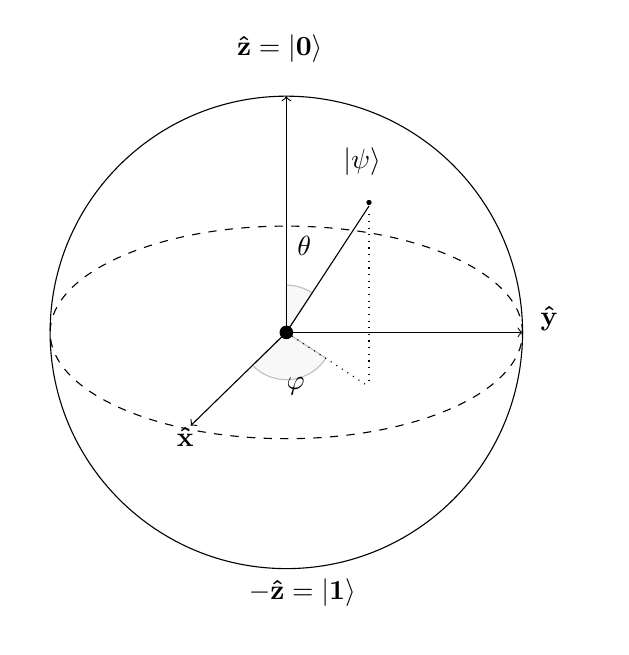
\begin{tikzpicture}[scale=1.5]
    \clip(-2.19,-2.49) rectangle (2.66,2.58);
    \draw [shift={(0,0)}, lightgray, fill, fill opacity=0.1] (0,0) -- (56.7:0.4) arc (56.7:90.:0.4) -- cycle;
    \draw [shift={(0,0)}, lightgray, fill, fill opacity=0.1] (0,0) -- (-135.7:0.4) arc (-135.7:-33.2:0.4) -- cycle;
    \draw(0,0) circle (2cm);
    \draw [rotate around={0.:(0.,0.)},dash pattern=on 3pt off 3pt] (0,0) ellipse (2cm and 0.9cm);
    \draw (0,0)-- (0.70,1.07);
    \draw [->] (0,0) -- (0,2);
    \draw [->] (0,0) -- (-0.81,-0.79);
    \draw [->] (0,0) -- (2,0);
    \draw [dotted] (0.7,1)-- (0.7,-0.46);
    \draw [dotted] (0,0)-- (0.7,-0.46);
    \draw (-0.08,-0.3) node[anchor=north west] {$\varphi$};
    \draw (0.01,0.9) node[anchor=north west] {$\theta$};
    \draw (-1.01,-0.72) node[anchor=north west] {$\mathbf {\hat{x}}$};
    \draw (2.07,0.3) node[anchor=north west] {$\mathbf {\hat{y}}$};
    \draw (-0.5,2.6) node[anchor=north west] {$\mathbf {\hat{z}=|0\rangle}$};
    \draw (-0.4,-2) node[anchor=north west] {$-\mathbf {\hat{z}=|1\rangle}$};
    \draw (0.4,1.65) node[anchor=north west] {$|\psi\rangle$};
    \scriptsize
    \draw [fill] (0,0) circle (1.5pt);
    \draw [fill] (0.7,1.1) circle (0.5pt);
  \end{tikzpicture}
  \centering
\caption{\label{fig:bloch_sphere}The Bloch Sphere}
\end{figure}
\vspace{5mm}

\noindent
These qubit states can be expressed in column matrices as:
\vspace{5mm}

\begin{equation}
\ket{0} = \begin{pmatrix}1 \\ 0 \end{pmatrix} \ \ \text{and} \ \ \ket{1} = \begin{pmatrix} 0 \\ 1 \end{pmatrix}
\end{equation}

\vspace{5mm}

\noindent
The state of a quantum system can be represented as the spin, energy, angular momentum and magnetic moment of an elementary particle. However for the sake of brevity the state $\ket{0}$ and $\ket{1}$ will denote spin up and spin down of the electron in this report.
\vspace{10mm}

\subsection{Quantum Register}
\vspace{5mm}

\noindent
The qubits in a quantum computer are stored in a quantum register. The size of the quantum register is dictated by the number of qubits. 
\vspace{5mm}

\noindent
The vector state of the quantum register $\mathcal{H}$ with $n$ qubits can be expressed in tensor product \cite{noauthor_lecture_nodate}:
\vspace{5mm}


\qquad $\mathcal{H} = \mathbb{C}^{2\otimes N} = \mathbb{C}^2 \otimes\mathbb{C}^2 ....\otimes\mathbb{C}^2 = \mathbb{C}^{2^N} $ , \  where the qubits are in 2-dimensional complex spaces $\mathbb{C}$.
\vspace{5mm}

\noindent
Each qubit has an index in this register, starting at index 0 and counting up by 1. So, a system with 5 qubits, for example, has a qubit register that has a width of 5 and indexed by 0, 1, 2, 3 and 4.

\subsection{Tensor Product}
\vspace{5mm}

\noindent
Tensor product is used as a function which combines elements of two or more vector spaces to yield an additional vector space. 
\vspace{5mm}

\noindent
Tensor products are distributive and associative and shown here are the tensor products of two qubits $\ket{x}$ and $\ket{y}$, for $\alpha , \beta \in \mathbb{C}$, which obey such properties in the Hilbert space (complex vector space)\cite{noauthor_lecture_nodate}:
\vspace{5mm}


\begin{equation}
\alpha\ket{x} \otimes \beta\ket{y} = \alpha\beta\ket{xy}
\end{equation}
\vspace{5mm}


\begin{equation}\ket{x} \otimes (\ket{y} + \ket{z}) = \ket{x}\otimes \ket{y} + \ket{x}\otimes\ket{z}
\end{equation}
\vspace{5mm}


\begin{equation}
(\ket{x} + \ket{y}) \otimes \ket{z} = \ket{x}\otimes \ket{z} + \ket{y}\otimes\ket{z}
\end{equation}
\vspace{5mm}


\begin{equation}
(\ket{x} \otimes \ket{y}) \otimes \ket{z} = \ket{x} \otimes (\ket{y} \otimes\ket{z}) = \ket{x} \otimes \ket{y} \otimes\ket{z}
\end{equation}
\vspace{10mm}

The basis for the tensor product space is given by the product of single qubit basis states.
\vspace{5mm}

\begin{center}
$\ket{0}_2 \otimes \ket{0}_1 \otimes \ket{0}_0 = \ket{000} = \ket{0}$
\vspace{5mm}

$\ket{0}_2 \otimes \ket{0}_1 \otimes \ket{1}_0 = \ket{001} = \ket{1}$
\vspace{5mm}

$\cdots \cdots $

$\cdots \cdots$

$\cdots \cdots$
\vspace{5mm}

$\ket{1}_2 \otimes \ket{1}_1 \otimes \ket{1}_0 = \ket{111} = \ket{7}$
\end{center}
\vspace{5mm}

Little endian notation is used to represent the qubit from right to left starting with the subscript 0.

For ease of interpretation, the binary to decimal conversion is written on the right hand side. 
\vspace{10mm}

\subsection{Linear Algebra}
\vspace{5mm}

\noindent
Linear algebra is the language of quantum computing. It is the study of vector spaces and of linear operations on vector
spaces (Hilbert space).
\vspace{5mm}

\noindent
A generic quantum state $\ket{\psi}$ can be described as a linear combination of basis states such as \cite{noauthor_lecture_nodate}:
\vspace{5mm}


\begin{equation}
\ket{\psi} = \alpha_0\ket{0} + ... + \alpha_j\ket{j} = \sum\limits_{j = 0}^{j} \alpha_j\ket{j} , \ \text{for} \ \alpha_j \in \mathbb{C}
\end{equation}
\vspace{5mm}

\noindent
Due to the probabilistic nature of quantum mechanics, the state must be normalised, i.e $\sum\limits_j |\alpha_j|^2 = 1$
\vspace{5mm}

\noindent
The action of quantum operators on a state is linear. For a quantum operator $U$ acting on some state $\ket{x}$ and $\ket{y}$ can be expressed as:
\vspace{5mm}

\noindent
\begin{equation}
U(\alpha\ket{x} + \beta\ket{y}) = \alpha U\ket{x} + \beta U\ket{x} , \ \text{for} \ \alpha, \beta \in \mathbb{C}
\end{equation}
\vspace{5mm}

\noindent
The action of a quantum linear operator on a basis state determines the type of operator it is. It can also act on multiple or superposition of basis states:
\vspace{5mm}

\noindent
\begin{equation}
U \sum\limits_j \alpha_j \ket{j} = \sum\limits_j \alpha_j U\ket{j}
\end{equation}
\vspace{10mm}

\subsection{Matrix Operation}
\vspace{5mm}

\noindent
Linear operators $U$ acting on some basis states can be written in matrix form \cite{noauthor_lecture_nodate}:
\vspace{5mm}

\begin{equation}
U_{kj} = \bra{k}U\ket{j} \ , \text{for some basis state} \ket{j} \text{and} \ket{k} 
\end{equation}
\vspace{5mm}

\noindent
By using the Completeness Relation of quantum mechanics:
\vspace{5mm}

\begin{equation}
U\ket{j} = \underbrace{\sum\limits_k\ket{k}\bra{k}}_{ = 1} U\ket{j} = \sum\limits_k \ket{k} U_{kj}    
\end{equation}
\vspace{5mm}

\noindent
Multiple linear operators applied on a basis state can be written as:
\vspace{5mm}

\begin{equation}
UV\ket{k} = U\sum\limits_k \ket{k}V_{kj} = \sum\limits_l\ket{l} \sum\limits_k U_{lk} V_{kj} = \sum\limits_l(UV)_{lj}
\end{equation}
\vspace{5mm}

\noindent
The linear operator $U$ acting on the coefficient $\alpha$ of the vector state $\ket{\psi}$ can be expressed:
\vspace{5mm}

\begin{equation}
\alpha' = U\alpha
\end{equation}
\vspace{5mm}

\noindent
And on the state:
\vspace{5mm}

\begin{equation}
\ket{\psi'} = U\ket{\psi}
\end{equation}
\vspace{5mm}

\noindent
Additionally, all quantum operators (quantum gates) are unitary with the exception of measurement and reset operators. 
\vspace{5mm}

\noindent
A quantum operator $U$ has its conjugate transpose (adjoint) which can be expressed as $U^{\dagger}$.
\vspace{5mm}

\noindent
The unitary operator has the following property\cite{noauthor_unitary_2022}:
\vspace{5mm}

\begin{equation}
UU^{\dagger} = UU^{-1} = 1    
\end{equation}
\vspace{5mm}

\noindent
Another consequence of unitarity is that it preserves the inner product between two arbitrary states $\braket{\phi}{\psi}$. For example apply the unitary operator $U$ to two states $\ket{\phi}$ and $\ket{\psi}$:
\vspace{5mm}

\begin{equation}
\bra{\phi} U^{\dagger} U\ket{\psi} = \braket{\phi}{\psi}
\end{equation}
\vspace{5mm}

\noindent
the inner product of the resulting states is exactly the same,
\vspace{10mm}


\subsection{Gates and Operators}
\vspace{5mm}

Quantum gates are unitary quantum operators and are described as unitary matrices relative to some basis states.
\vspace{5mm}

\noindent
The following are some of the common types of quantum gates\cite{voorhoede_pauli-x_nodate} which will be used in constructing the Grover's circuit.
\vspace{5mm}

\textbf{Hadamard Gate}: \qquad $H = \frac{1}{\sqrt{2}} \begin{pmatrix} 1 & 1 \\ 1 & -1 \end{pmatrix}$
\vspace{5mm}

\noindent
The Hadamard gate creates a superposition states when acted on a state:
\vspace{5mm}


\begin{equation}
H\ket{0} = \frac{1}{\sqrt{2}} (\ket{0} + \ket{1}), \ \ H\ket{1} = \frac{1}{\sqrt{2}}(\ket{0} - \ket{1})   
\end{equation}
\vspace{5mm}

\noindent
This can then be generalised as:
\vspace{5mm}

\begin{equation}
H\ket{j} = \frac{-1^j\ket{j} + \ket{1 - j}}{\sqrt{2}} 
\end{equation}
\vspace{5mm}


\textbf{Pauli X Gate}: \qquad $X = \begin{pmatrix} 0 & 1 \\ 1 & 0 \end{pmatrix}$
\vspace{5mm}


\begin{equation}
X\ket{0} = \ket{1} , \ \ X\ket{1} = \ket{0}
\end{equation}
\vspace{5mm}

\noindent
The Pauli X Gate acts very similar to a classical NOT gate. This effect of this gate is also known as bit flip. The gate is a single qubit rotation around the x-axis by $\pi$.
\vspace{5mm}


\textbf{Pauli Y Gate}: \qquad $Y = \begin{pmatrix} 0 & -i \\ i & 0 \end{pmatrix}$
\vspace{5mm}


\begin{equation}
Y\ket{0} = i\ket{1} , \ \ Y\ket{1} = -i\ket{0}
\end{equation}
\vspace{5mm}

\noindent
The Pauli Y Gate rotates a single qubit in the y (complex)-axis by $\pi$.
\vspace{5mm}


\textbf{Pauli Z Gate}: \qquad $Z = \begin{pmatrix} 1 & 0 \\ 0 & -1 \end{pmatrix}$
\vspace{5mm}


\begin{equation}
Z\ket{0} = \ket{0} , \ \ Z\ket{1} = -\ket{1}  
\end{equation}
\vspace{5mm}

\noindent
The Pauli-Z gate is a single qubit rotation through $\pi$ radians around the z-axis. The effect of the Pauli Z Gate is also known as phase-flip.
\vspace{5mm}

\textbf{Controlled Not/CNOT Gate}: \qquad CNOT = $\begin{pmatrix} 1 & 0 & 0 & 0 \\ 0 & 1 & 0 & 0 \\ 0 & 0 & 0 & 1 \\ 0 & 0 & 1 & 0 \end{pmatrix}$
\vspace{5mm}

\noindent
The CNOT Gate is a two qubit gate which takes the first qubit as the control qubit and the second qubit as the target qubit.
\vspace{5mm}

\noindent
It leaves the control qubit unchanged and performs the Pauli X Gate to the target qubit if and only if when the control qubit is $\ket{1}$ and leaves the target qubit unchanged when the control qubit is $\ket{0}$.
\vspace{5mm}

\textbf{Controlled Z/CZ Gate}: \qquad CZ = $\begin{pmatrix} 1 & 0 & 0 & 0 \\ 0 & 1 & 0 & 0 \\ 0 & 0 & 1 & 0 \\ 0 & 0 & 0 & -1 \end{pmatrix}$
\vspace{5mm}

\noindent
The CZ Gate is a two qubit gate which takes the first qubit as the control qubit and the second qubit as the target qubit.
\vspace{5mm}

\noindent
It leaves the control qubit unchanged and performs the Pauli Z Gate to the target qubit if and only if when the control qubit is $\ket{1}$ and leaves the target qubit unchanged when the control qubit is $\ket{0}$.
\pagebreak

\textbf{Phase Shift Gates}: \qquad $ P(\varphi) = \begin{pmatrix} 1 & 0 \\ 0 & e^{i\varphi} \end{pmatrix}$ 
\vspace{5mm}

\begin{equation}
P(\varphi)\ket{0} = \ket{0} \ \text{and} \ P(\varphi)\ket{1} = e^{i\varphi}\ket{1} 
\end{equation}

\noindent
The phase shift gate modifies the phase of the quantum state and is equivalent to tracing a horizontal circle on the Bloch Sphere (see Figure \ref{fig:bloch_sphere}) by $\varphi$ radians\cite{noauthor_quantum_nodate}. 

\pagebreak

\section{Grover's Algorithm}
\subsection{Introduction}

The Grover's Algorithm is a quantum search algorithm which increases quadratically the speed of unstructured search\cite{noauthor_grovers_nodate}. It uses  amplitude amplification to search an unstructured set of $N$ elements/items. 

\subsection{Unstructured Search}
\vspace{10mm}

\begin{figure}[h]
  \begin{center}

    \tikzset{every picture/.style={line width=0.75pt}} %set default line width to 0.75pt        

    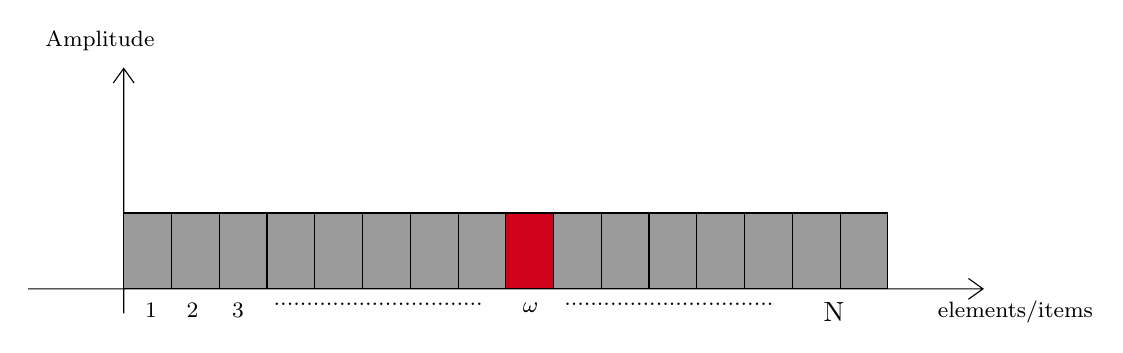
\begin{tikzpicture}[x=0.75pt,y=0.75pt,yscale=-1,xscale=1]
      %uncomment if require: \path (0,310); %set diagram left start at 0, and has height of 310

      %Shape: Axis 2D [id:dp7326811016330554] 
      \draw  (54,256.57) -- (514,256.57)(100,150.37) -- (100,268.37) (507,251.57) -- (514,256.57) -- (507,261.57) (95,157.37) -- (100,150.37) -- (105,157.37)  ;
      %Shape: Rectangle [id:dp9165080769461678] 
      \draw  [fill={rgb, 255:red, 155; green, 155; blue, 155 }  ,fill opacity=1 ] (100,220) -- (123.02,220) -- (123.02,256.57) -- (100,256.57) -- cycle ;
      %Shape: Rectangle [id:dp6197087457024866] 
      \draw  [fill={rgb, 255:red, 155; green, 155; blue, 155 }  ,fill opacity=1 ] (123.02,220) -- (146.04,220) -- (146.04,256.57) -- (123.02,256.57) -- cycle ;
      %Shape: Rectangle [id:dp5818508515663341] 
      \draw  [fill={rgb, 255:red, 155; green, 155; blue, 155 }  ,fill opacity=1 ] (146.04,220) -- (169.06,220) -- (169.06,256.57) -- (146.04,256.57) -- cycle ;
      %Shape: Rectangle [id:dp6466988498042014] 
      \draw  [fill={rgb, 255:red, 155; green, 155; blue, 155 }  ,fill opacity=1 ] (169.06,220) -- (192.08,220) -- (192.08,256.57) -- (169.06,256.57) -- cycle ;
      %Shape: Rectangle [id:dp9241747490680354] 
      \draw  [fill={rgb, 255:red, 155; green, 155; blue, 155 }  ,fill opacity=1 ] (192.08,220) -- (215.1,220) -- (215.1,256.57) -- (192.08,256.57) -- cycle ;
      %Shape: Rectangle [id:dp6900943731279547] 
      \draw  [fill={rgb, 255:red, 155; green, 155; blue, 155 }  ,fill opacity=1 ] (215.1,220) -- (238.12,220) -- (238.12,256.57) -- (215.1,256.57) -- cycle ;
      %Shape: Rectangle [id:dp9784662305616809] 
      \draw  [fill={rgb, 255:red, 155; green, 155; blue, 155 }  ,fill opacity=1 ] (238.12,220) -- (261.14,220) -- (261.14,256.57) -- (238.12,256.57) -- cycle ;
      %Shape: Rectangle [id:dp3189854749942387] 
      \draw  [fill={rgb, 255:red, 155; green, 155; blue, 155 }  ,fill opacity=1 ] (261.14,220) -- (284.16,220) -- (284.16,256.57) -- (261.14,256.57) -- cycle ;
      %Shape: Rectangle [id:dp19644432939638312] 
      \draw  [fill={rgb, 255:red, 208; green, 2; blue, 27 }  ,fill opacity=1 ] (284.04,220) -- (307.06,220) -- (307.06,256.57) -- (284.04,256.57) -- cycle ;
      %Shape: Rectangle [id:dp4454731461786199] 
      \draw  [fill={rgb, 255:red, 155; green, 155; blue, 155 }  ,fill opacity=1 ] (307.06,220) -- (330.08,220) -- (330.08,256.57) -- (307.06,256.57) -- cycle ;
      %Shape: Rectangle [id:dp8963311487850567] 
      \draw  [fill={rgb, 255:red, 155; green, 155; blue, 155 }  ,fill opacity=1 ] (330.08,220) -- (353.1,220) -- (353.1,256.57) -- (330.08,256.57) -- cycle ;
      %Shape: Rectangle [id:dp8621164913285171] 
      \draw  [fill={rgb, 255:red, 155; green, 155; blue, 155 }  ,fill opacity=1 ] (353.1,220) -- (376.12,220) -- (376.12,256.57) -- (353.1,256.57) -- cycle ;
      %Shape: Rectangle [id:dp7667099225825136] 
      \draw  [fill={rgb, 255:red, 155; green, 155; blue, 155 }  ,fill opacity=1 ] (376.12,220) -- (399.14,220) -- (399.14,256.57) -- (376.12,256.57) -- cycle ;
      %Shape: Rectangle [id:dp1405504024872024] 
      \draw  [fill={rgb, 255:red, 155; green, 155; blue, 155 }  ,fill opacity=1 ] (399.14,220) -- (422.16,220) -- (422.16,256.57) -- (399.14,256.57) -- cycle ;
      %Shape: Rectangle [id:dp6549374163542783] 
      \draw  [fill={rgb, 255:red, 155; green, 155; blue, 155 }  ,fill opacity=1 ] (422.16,220) -- (445.18,220) -- (445.18,256.57) -- (422.16,256.57) -- cycle ;
      %Shape: Rectangle [id:dp26369533307147797] 
      \draw  [fill={rgb, 255:red, 155; green, 155; blue, 155 }  ,fill opacity=1 ] (445.18,220) -- (468.2,220) -- (468.2,256.57) -- (445.18,256.57) -- cycle ;

      % Text Node
      \draw (491,261) node [anchor=north west][inner sep=0.75pt]   [align=left] {{\footnotesize elements/items}};
      % Text Node
      \draw (61,131) node [anchor=north west][inner sep=0.75pt]   [align=left] {{\footnotesize Amplitude}};
      % Text Node
      \draw (109,262) node [anchor=north west][inner sep=0.75pt]  [font=\footnotesize] [align=left] {1};
      % Text Node
      \draw (129,262) node [anchor=north west][inner sep=0.75pt]  [font=\footnotesize] [align=left] {2};
      % Text Node
      \draw (171,262) node [anchor=north west][inner sep=0.75pt]  [font=\footnotesize] [align=left] {................................};
      % Text Node
      \draw (151,262) node [anchor=north west][inner sep=0.75pt]  [font=\footnotesize] [align=left] {3};
      % Text Node
      \draw (311,262) node [anchor=north west][inner sep=0.75pt]  [font=\footnotesize] [align=left] {................................};
      % Text Node
      \draw (291,262) node [anchor=north west][inner sep=0.75pt]  [font=\footnotesize] [align=left] {$\displaystyle \omega $};
      % Text Node
      \draw (436,262) node [anchor=north west][inner sep=0.75pt]   [align=left] {N};

    \end{tikzpicture}    
  \end{center}
  \caption{\label{fig:intial_quantum_state} The initial quantum state}
\end{figure}

\vspace{10mm}
\noindent
An unstructured search through a list of items using Grover's Algorithm can be illustrated in Figure1. In this instance, $\omega$ the red block, represents the item which we want to find and $N$ represents the number of items in the list. 
\vspace{5mm}

\noindent
On classical computation, $\omega$ must check at least on average $O(N/2)$ entries of the list which gives $\frac{1}{2}$ the probability of finding $\omega$ or worse the entire N elements in the list.
With Grover's Algorithm, only $O(\sqrt{N})$ steps are required to find $\omega$.
\vspace{5mm}

\noindent
For an $N$ item search problem with $M$ number of solutions, the required number of times of searches will be $O(\sqrt{\frac{N}{M}})$\cite{nielsen_quantum_2010}.
\pagebreak

\subsection{The Oracle} \label{The Oracle}
\vspace{5mm}

Let's suppose the function $f$ of $N$ integer such that $f:\{0,1, 2,...., N-1\} \rightarrow{\{0,1\}}$. 
\vspace{5mm}

\noindent
The integers in the domain corresponds to the indices of the list and $f(x) =1$ if and only if $x$ corresponds to the item which is to be searched. Conversely, $f(x) =0$ for $x$ not corresponding to the item to be searched. 
\vspace{5mm}

\noindent
There will be only one value of $x$ which satisfies $f(x)=1$ and this index corresponds to item $\omega$\cite{noauthor_grovers_2022}.
\vspace{5mm}

\noindent
So $f$ can be accessed with a unitary operator $U_{\omega}$ of  an oracle which satisfies:
\vspace{5mm}

\begin{equation}
\begin{cases}
      U_{\omega}\ket{x} = -\ket{x}  & \text{for} \ x = \omega, \ f(x) =1 \\
       U_{\omega}\ket{x} = \ket{x}  & \text{for} \ x \neq \omega, \ f(x) = 0 \\
\end{cases}  
\end{equation}

\vspace{5mm}

The oracle function of a two qubit system is defined as\cite{j_quantum_2020}:
\vspace{5mm}

\begin{equation}
\ket{x} \otimes \ket{q} \rightarrow{O_f} \ket{x} \otimes \ket{q \oplus f(x)} \footnote{$\otimes$ denotes tensor product and $\oplus$ denotes denotes addition modulo 2}  
\end{equation}

\vspace{5mm}

\begin{equation}
\ket{q} = \frac{\ket{0} - \ket{1}}{\sqrt{2}}
\end{equation}
\vspace{5mm}

Substitute $\ket{q}$ into the oracle function $O_f$:
\vspace{5mm}

\begin{equation}
 O\ket{x}\frac{\ket{0} - \ket{1}}{\sqrt{2}} \rightarrow \ket{x} \frac{\ket{f(x) \oplus 0} - \ket{f(x) \oplus 1}}{\sqrt{2}}    
\end{equation}
\vspace{5mm}

\begin{equation}
\text{if} \ f(x) =1 \rightarrow \ket{x}\frac{\ket{f(x) \oplus0} - \ket{f(x) \oplus1}}{\sqrt{2}}   
\end{equation}
\vspace{5mm}

\begin{equation}
\text{if} \ f(x) =1 \rightarrow \ket{x}\frac{\ket{1 \oplus 0} - \ket{1 \oplus 1}}{\sqrt{2}} = -\ket{x}\frac{\ket{0} - \ket{1}}{\sqrt{2}}    
\end{equation}
\vspace{5mm}

\begin{equation}
\text{if} \ f(x) =0 \rightarrow \ket{x}\frac{\ket{0 \oplus 0} - \ket{0 \oplus 1}}{\sqrt{2}} = \ket{x}\frac{\ket{0} - \ket{1}}{\sqrt{2}}    
\end{equation}
\vspace{5mm}

\noindent
When $f(x) = 1 $, the amplitude $\ket{x}$ changed to negative and remains unchanged when $f(x) = 0$.
\vspace{5mm}

\noindent
The oracle takes the form of a diagonal matrix $U_{\omega}$
\vspace{5mm}
\noindent
For example, in a three qubit state, we want to look for the number 6 which corresponds to $\ket{110}$. In matrix form $\omega =6$ will be:
\vspace{5mm}

\qquad $ U_\omega = \begin{bmatrix}

1 & 0 & 0 & 0 & 0& 0 & 0& 0 \\
0 & 1 & 0 & 0 & 0& 0 & 0& 0 \\
0 & 0 & 1 & 0 & 0& 0 & 0& 0 \\
0 & 0 & 0 & 1 & 0& 0 & 0& 0 \\
0 & 0 & 0 & 0 & 1& 0 & 0& 0 \\
0 & 0 & 0 & 0 & 0& 1 & 0& 0 \\
0 & 0 & 0 & 0 & 0& 0 & -1& 0 \\
0 & 0 & 0 & 0 & 0& 0 & 0& 1 \\

\end{bmatrix}$
\vspace{5mm}

Hence the oracle can be described as:
\vspace{5mm}

\begin{equation}
U_\omega\ket{x} = (-1)^{f(x)} \ket{x}    
\end{equation}
\vspace{5mm}

This is essentially a reflection on the state $\ket{x}$.

\pagebreak

\subsection{How The Algorithm Works} \label{How the Algorithm Works}
\vspace{5mm}

\textbf{Step 1:}
\vspace{5mm}
\noindent
The sequence of the Grover's Algorithm starts out with a uniform superposition state $\ket{s}$\cite{noauthor_grovers_nodate}:
\vspace{5mm}

\begin{equation}
\ket{s}= H^{\otimes n} \ket{0}^n = \frac{1}{\sqrt{2^n}}\sum\limits_{x \in \{0,1\}^n}\ket{x}
\end{equation}
\vspace{5mm}

\qquad For $N = 2^n$ , where $n$ is the number of qubits.
\vspace{5mm}


\begin{figure}[h]
  \begin{subfigure}{.5\textwidth}
    \centering
    \tikzset{every picture/.style={line width=0.75pt}} %set default line width to 0.75pt

    \begin{tikzpicture}[x=0.75pt,y=0.75pt,yscale=-1,xscale=1]
      % uncomment if require: \path (0,300); %set diagram left start at 0, and has height of 300

      %Shape: Axis 2D [id:dp05560542711234939] 
      \draw  (50,247.9) -- (308,247.9)(75.8,112) -- (75.8,263) (301,242.9) -- (308,247.9) -- (301,252.9) (70.8,119) -- (75.8,112) -- (80.8,119)  ;
      %Shape: Boxed Line [id:dp13553556978051007] 
      \draw    (75.8,247.9) -- (298.07,185.84) ;
      \draw [shift={(300,185.3)}, rotate = 164.4] [color={rgb, 255:red, 0; green, 0; blue, 0 }  ][line width=0.75]    (10.93,-3.29) .. controls (6.95,-1.4) and (3.31,-0.3) .. (0,0) .. controls (3.31,0.3) and (6.95,1.4) .. (10.93,3.29)   ;

      % Text Node
      \draw (82,87.4) node [anchor=north west][inner sep=0.75pt]    {$\ket{\omega }$};
      % Text Node
      \draw (306,167.4) node [anchor=north west][inner sep=0.75pt]    {$\ket{s}$};
      % Text Node
      \draw (307,253.4) node [anchor=north west][inner sep=0.75pt]    {$\ket{s'}$};
      % Text Node
      \draw (181,220.4) node [anchor=north west][inner sep=0.75pt]    {$\theta $};

    \end{tikzpicture}

    \caption{\label{fig:grover_step_1a} Grover's Algorithm Step 1a}
  \end{subfigure}%
  \begin{subfigure}{.5\textwidth}
    \centering
    \tikzset{every picture/.style={line width=0.75pt}} %set default line width to 0.75pt        

    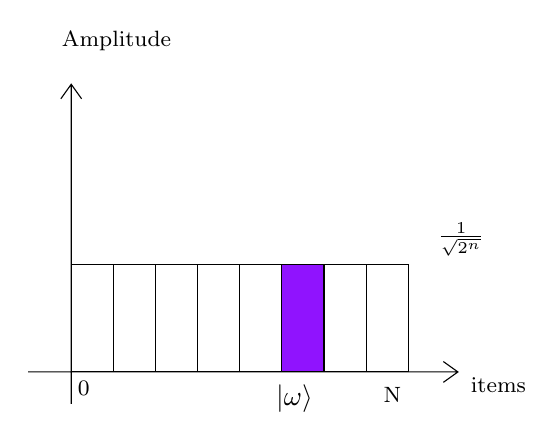
\begin{tikzpicture}[x=0.75pt,y=0.75pt,yscale=-1,xscale=1]
      %uncomment if require: \path (0,300); %set diagram left start at 0, and has height of 300

      %Shape: Axis 2D [id:dp29246180096889995] 
      \draw  (390,249.6) -- (597,249.6)(410.7,111) -- (410.7,265) (590,244.6) -- (597,249.6) -- (590,254.6) (405.7,118) -- (410.7,111) -- (415.7,118)  ;
      %Shape: Rectangle [id:dp09588343067912675] 
      \draw   (410.7,198) -- (431,198) -- (431,249.6) -- (410.7,249.6) -- cycle ;
      %Shape: Rectangle [id:dp06589745305688277] 
      \draw   (431,198) -- (451.3,198) -- (451.3,249.6) -- (431,249.6) -- cycle ;
      %Shape: Rectangle [id:dp1570793013008731] 
      \draw   (451.3,198) -- (471.6,198) -- (471.6,249.6) -- (451.3,249.6) -- cycle ;
      %Shape: Rectangle [id:dp04465276081897107] 
      \draw   (471.6,198) -- (491.9,198) -- (491.9,249.6) -- (471.6,249.6) -- cycle ;
      %Shape: Rectangle [id:dp3205832207723005] 
      \draw   (491.9,198) -- (512.2,198) -- (512.2,249.6) -- (491.9,249.6) -- cycle ;
      %Shape: Rectangle [id:dp7965850817244042] 
      \draw  [fill={rgb, 255:red, 144; green, 19; blue, 254 }  ,fill opacity=1 ] (512.2,198) -- (532.5,198) -- (532.5,249.6) -- (512.2,249.6) -- cycle ;
      %Shape: Rectangle [id:dp41205715411636223] 
      \draw   (532.5,198) -- (552.8,198) -- (552.8,249.6) -- (532.5,249.6) -- cycle ;
      %Shape: Rectangle [id:dp6260805143227606] 
      \draw   (552.8,198) -- (573.1,198) -- (573.1,249.6) -- (552.8,249.6) -- cycle ;

      % Text Node
      \draw (405,84) node [anchor=north west][inner sep=0.75pt]   [align=left] {{\footnotesize Amplitude}};
      % Text Node
      \draw (412.7,252.6) node [anchor=north west][inner sep=0.75pt]   [align=left] {{\footnotesize 0}};
      % Text Node
      \draw (586,176.4) node [anchor=north west][inner sep=0.75pt]  [font=\footnotesize]  {$\frac{1}{\sqrt{2^{n}}}$};
      % Text Node
      \draw (560,256) node [anchor=north west][inner sep=0.75pt]   [align=left] {{\footnotesize N}};
      % Text Node
      \draw (602,251) node [anchor=north west][inner sep=0.75pt]   [align=left] {{\footnotesize items}};
      % Text Node
      \draw (508.2,254.4) node [anchor=north west][inner sep=0.75pt]    {$\ket{\omega }$};

    \end{tikzpicture}
    \caption{\label{fig:grover_step_1b} Grover's Algorithm Step 1b}
  \end{subfigure}
  \caption{\label{fig:grover_step_1} Grover's Algorithm Step 1}
\end{figure}
\vspace{5mm}

Figure \ref{fig:grover_step_1a} shows a two dimensional plane spanned by $\ket{\omega}$ and $\ket{s'}$. In this representation, it can be written:
\vspace{5mm}

\begin{equation}
\ket{s} = \sin\theta\ket{\omega} + \cos\theta\ket{s'}   
\end{equation}
\vspace{5mm}

\begin{equation}
\sin\theta = \frac{1}{\sqrt{2^n}}    
\end{equation}
\vspace{5mm}

Where the amplitude of $\ket{s}$ is as shown in Figure \ref{fig:grover_step_1b}.
\pagebreak

\textbf{Step 2:}
\vspace{5mm}
Next apply the reflection oracle $U_\omega$ to the state $\ket{s}$.
\vspace{5mm}


\begin{figure}[h]
  \begin{subfigure}{0.5\textwidth}
    \centering
    \tikzset{every picture/.style={line width=0.75pt}} %set default line width to 0.75pt        
    
    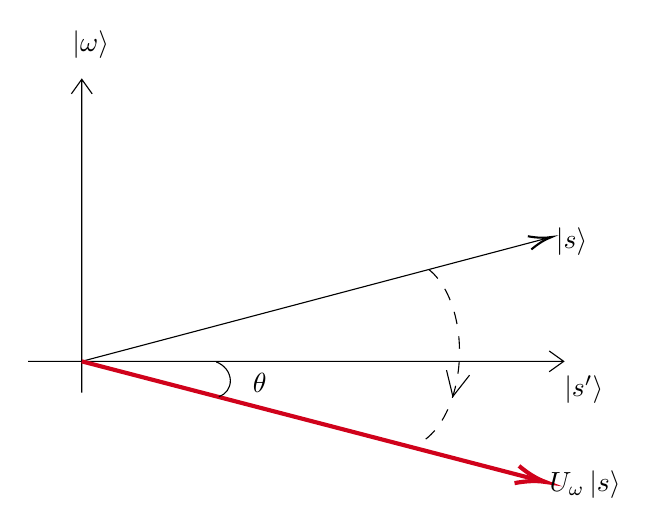
\begin{tikzpicture}[x=0.75pt,y=0.75pt,yscale=-1,xscale=1]
        %uncomment if require: \path (0,421); %set diagram left start at 0, and has height of 421
        
        %Shape: Axis 2D [id:dp9468133521588677] 
        \draw  (50,250.9) -- (308,250.9)(75.8,115) -- (75.8,266) (301,245.9) -- (308,250.9) -- (301,255.9) (70.8,122) -- (75.8,115) -- (80.8,122)  ;
        %Shape: Boxed Line [id:dp05857323871196929] 
        \draw    (75.8,250.9) -- (300.2,191.51) ;
        \draw [shift={(302.13,191)}, rotate = 165.18] [color={rgb, 255:red, 0; green, 0; blue, 0 }  ][line width=0.75]    (10.93,-3.29) .. controls (6.95,-1.4) and (3.31,-0.3) .. (0,0) .. controls (3.31,0.3) and (6.95,1.4) .. (10.93,3.29)   ;
        %Shape: Boxed Line [id:dp6041685570388957] 
        \draw [color={rgb, 255:red, 208; green, 2; blue, 27 }  ,draw opacity=1 ][fill={rgb, 255:red, 74; green, 144; blue, 226 }  ,fill opacity=1 ][line width=1.5]    (75.8,250.9) -- (296.23,308.24) ;
        \draw [shift={(299.13,309)}, rotate = 194.58] [color={rgb, 255:red, 208; green, 2; blue, 27 }  ,draw opacity=1 ][line width=1.5]    (14.21,-4.28) .. controls (9.04,-1.82) and (4.3,-0.39) .. (0,0) .. controls (4.3,0.39) and (9.04,1.82) .. (14.21,4.28)   ;
        %Shape: Arc [id:dp7847818797073434] 
        \draw  [draw opacity=0][dash pattern={on 4.5pt off 4.5pt}] (243.13,206.74) .. controls (255.6,216.75) and (261.2,241.7) .. (255.64,263.91) .. controls (252.12,278.01) and (244.9,287.75) .. (236.73,291.16) -- (231.03,247.47) -- cycle ; \draw  [dash pattern={on 4.5pt off 4.5pt}] (243.13,206.74) .. controls (255.6,216.75) and (261.2,241.7) .. (255.64,263.91) .. controls (252.12,278.01) and (244.9,287.75) .. (236.73,291.16) ;  
        \draw   (262.62,257.57) -- (254.59,267.79) -- (251.53,255.15) ;
        %Shape: Arc [id:dp2964811498005937] 
        \draw  [draw opacity=0] (140.64,251.2) .. controls (144.47,252.64) and (147.27,256.11) .. (147.38,260.04) .. controls (147.48,263.72) and (145.19,266.77) .. (141.81,268.01) -- (137.59,259.56) -- cycle ; \draw   (140.64,251.2) .. controls (144.47,252.64) and (147.27,256.11) .. (147.38,260.04) .. controls (147.48,263.72) and (145.19,266.77) .. (141.81,268.01) ;  
        
        % Text Node
        \draw (70,90.4) node [anchor=north west][inner sep=0.75pt]    {$\ket{\omega }$};
        % Text Node
        \draw (303,185.4) node [anchor=north west][inner sep=0.75pt]    {$\ket{s}$};
        % Text Node
        \draw (307,256.4) node [anchor=north west][inner sep=0.75pt]    {$\ket{s'}$};
        % Text Node
        \draw (157,255.4) node [anchor=north west][inner sep=0.75pt]    {$\theta $};
        % Text Node
        \draw (300,302.4) node [anchor=north west][inner sep=0.75pt]    {$U_{\omega }\ket{s}$};
    \end{tikzpicture}
    
    \caption{\label{fig:grover_step_2a} Grover's Algorithm Step 2a}
  \end{subfigure}%
  \begin{subfigure}{0.5\textwidth}
      \centering
      \tikzset{every picture/.style={line width=0.75pt}} %set default line width to 0.75pt        
      
      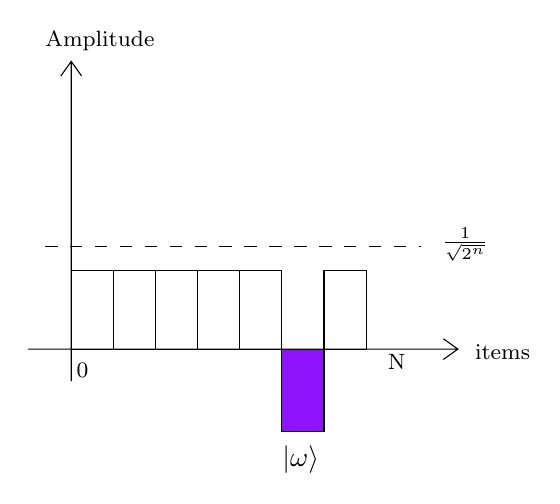
\begin{tikzpicture}[x=0.75pt,y=0.75pt,yscale=-1,xscale=1]
        %uncomment if require: \path (0,421); %set diagram left start at 0, and has height of 421
      
        %Shape: Axis 2D [id:dp13230548671390374] 
      \draw  (388,254.6) -- (595,254.6)(408.7,116) -- (408.7,270) (588,249.6) -- (595,254.6) -- (588,259.6) (403.7,123) -- (408.7,116) -- (413.7,123)  ;
%Shape: Rectangle [id:dp05277599517068765] 
\draw   (408.7,216.67) -- (429,216.67) -- (429,254.6) -- (408.7,254.6) -- cycle ;
%Shape: Rectangle [id:dp9567149694615606] 
\draw   (429,216.67) -- (449.3,216.67) -- (449.3,254.6) -- (429,254.6) -- cycle ;
%Shape: Rectangle [id:dp33156724904270707] 
\draw   (449.3,216.67) -- (469.6,216.67) -- (469.6,254.6) -- (449.3,254.6) -- cycle ;
%Shape: Rectangle [id:dp7921289702689205] 
\draw   (469.6,216.67) -- (489.9,216.67) -- (489.9,254.6) -- (469.6,254.6) -- cycle ;
%Shape: Rectangle [id:dp7099186384950043] 
\draw   (489.9,216.67) -- (510.2,216.67) -- (510.2,254.6) -- (489.9,254.6) -- cycle ;
%Shape: Rectangle [id:dp6243887993660082] 
\draw  [fill={rgb, 255:red, 144; green, 19; blue, 254 }  ,fill opacity=1 ] (510.2,254.6) -- (530.5,254.6) -- (530.5,294.33) -- (510.2,294.33) -- cycle ;
%Shape: Rectangle [id:dp9966482917344106] 
\draw   (530.5,216.67) -- (550.8,216.67) -- (550.8,254.6) -- (530.5,254.6) -- cycle ;
%Shape: Rectangle [id:dp29247452792340645] 
\draw  [dash pattern={on 4.5pt off 4.5pt}]  (396.13,205) -- (577.13,205) ;
        
        % Text Node
        \draw (395,100) node [anchor=north west][inner sep=0.75pt]   [align=left] {{\footnotesize Amplitude}};
        % Text Node
        \draw (410,260) node [anchor=north west][inner sep=0.75pt]   [align=left] {{\footnotesize 0}};
        % Text Node
        \draw (586,195) node [anchor=north west][inner sep=0.75pt]  [font=\footnotesize]  {$\frac{1}{\sqrt{2^{n}}}$};
        % Text Node
        \draw (560,256) node [anchor=north west][inner sep=0.75pt]   [align=left] {{\footnotesize N}};
        % Text Node
        \draw (602,251) node [anchor=north west][inner sep=0.75pt]   [align=left] {{\footnotesize items}};
        % Text Node
        \draw (509.2,300) node [anchor=north west][inner sep=0.75pt]    {$\ket{\omega }$};
    
      \end{tikzpicture}
      
      \caption{\label{fig:grover_step_2b} Grover's Algorithm Step 2b}
  \end{subfigure}
  \caption{\label{fig:grover_step_2} Grover's Algorithm Step 2}
\end{figure}
\vspace{5mm}

The reflection oracle $U_\omega$ can be expressed as:
\vspace{5mm}

\begin{equation}
U_\omega = 1 - 2\ket{\omega}\bra{\omega}    
\end{equation}

\vspace{5mm}

\begin{equation}
U_\omega \ket{s} = -\sin\theta\ket{\omega} +  \cos\theta\ket{\omega}    
\end{equation} 
\vspace{5mm}

\noindent
$U_{{\omega }}$ is a reflection at the hyperplane orthogonal to $\ket{\omega}$  for vectors in the plane spanned by $\ket{s'}$  and $\ket{\omega}$\cite{noauthor_grovers_2022}.
\vspace{5mm}

\noindent
Referring to Figure \ref{fig:grover_step_2a}, $\ket{s}$ is reflected about $\ket{s'}$. The reflection operation on $\ket{s}$ in the negative amplitude causes the overall positive average amplitude to decrease slightly as indicated by Figure \ref{fig:grover_step_2b}. 
\pagebreak

\textbf{Step 3:}
\vspace{5mm}

\begin{figure}[h]
  \begin{subfigure}{.5\textwidth}
    \centering
    \tikzset{every picture/.style={line width=0.75pt}} %set default line width to 0.75pt        

    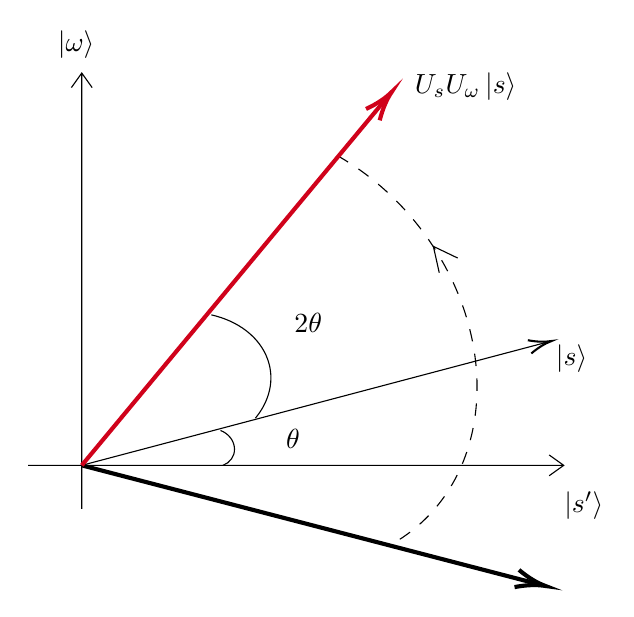
\begin{tikzpicture}[x=0.75pt,y=0.75pt,yscale=-1,xscale=1]
      %uncomment if require: \path (0,421); %set diagram left start at 0, and has height of 421

      %Shape: Axis 2D [id:dp1077584187321754] 
      \draw  (50,245) -- (308,245)(75.8,56) -- (75.8,266) (301,240) -- (308,245) -- (301,250) (70.8,63) -- (75.8,56) -- (80.8,63)  ;
      %Shape: Boxed Line [id:dp16066044861623174] 
      \draw    (75.8,245) -- (300.2,185.61) ;
      \draw [shift={(302.13,185.1)}, rotate = 165.18] [color={rgb, 255:red, 0; green, 0; blue, 0 }  ][line width=0.75]    (10.93,-3.29) .. controls (6.95,-1.4) and (3.31,-0.3) .. (0,0) .. controls (3.31,0.3) and (6.95,1.4) .. (10.93,3.29)   ;
      %Shape: Boxed Line [id:dp9706672155769875] 
      \draw [draw opacity=1 ][fill opacity=1 ][line width=1.5]    (75.8,245) -- (296.23,302.34) ;
      \draw [shift={(299.13,303.1)}, rotate = 194.58] [draw opacity=1 ][line width=1.5]    (14.21,-4.28) .. controls (9.04,-1.82) and (4.3,-0.39) .. (0,0) .. controls (4.3,0.39) and (9.04,1.82) .. (14.21,4.28)   ;
      %Shape: Arc [id:dp872952775851549] 
      \draw  [draw opacity=0][dash pattern={on 4.5pt off 4.5pt}] (198.95,95.79) .. controls (242.68,120.59) and (271.35,171.76) .. (265.48,219.88) .. controls (261.92,249.01) and (246.41,271.27) .. (224.47,283.34) -- (164.47,187.12) -- cycle ; \draw  [dash pattern={on 4.5pt off 4.5pt}] (198.95,95.79) .. controls (242.68,120.59) and (271.35,171.76) .. (265.48,219.88) .. controls (261.92,249.01) and (246.41,271.27) .. (224.47,283.34) ;  
      \draw   (248.03,152.19) -- (245.19,139.5) -- (256.91,145.12) ;
      %Shape: Arc [id:dp6976856692056519] 
      \draw  [draw opacity=0] (142.64,228.2) .. controls (146.47,229.64) and (149.27,233.11) .. (149.38,237.04) .. controls (149.48,240.72) and (147.19,243.77) .. (143.81,245.01) -- (139.59,236.56) -- cycle ; \draw   (142.64,228.2) .. controls (146.47,229.64) and (149.27,233.11) .. (149.38,237.04) .. controls (149.48,240.72) and (147.19,243.77) .. (143.81,245.01) ;  
      %Shape: Boxed Line [id:dp005988885245785669] 
      \draw [color={rgb, 255:red, 208; green, 2; blue, 27 }  ,draw opacity=1 ][fill={rgb, 255:red, 74; green, 144; blue, 226 }  ,fill opacity=1 ][line width=1.5]    (75.8,245) -- (223.22,67.41) ;
      \draw [shift={(225.13,65.1)}, rotate = 129.7] [color={rgb, 255:red, 208; green, 2; blue, 27 }  ,draw opacity=1 ][line width=1.5]    (14.21,-4.28) .. controls (9.04,-1.82) and (4.3,-0.39) .. (0,0) .. controls (4.3,0.39) and (9.04,1.82) .. (14.21,4.28)   ;
      %Shape: Arc [id:dp47337907989211914] 
      \draw  [draw opacity=0] (138.23,172.51) .. controls (151.09,175.41) and (161.57,183.15) .. (165.41,194.07) .. controls (168.83,203.79) and (166.27,214) .. (159.46,222.26) -- (123.73,205.22) -- cycle ; \draw   (138.23,172.51) .. controls (151.09,175.41) and (161.57,183.15) .. (165.41,194.07) .. controls (168.83,203.79) and (166.27,214) .. (159.46,222.26) ;  

      % Text Node
      \draw (63,34.4) node [anchor=north west][inner sep=0.75pt]    {$\ket{\omega }$};
      % Text Node
      \draw (303,185.4) node [anchor=north west][inner sep=0.75pt]    {$\ket{s}$};
      % Text Node
      \draw (307,256.4) node [anchor=north west][inner sep=0.75pt]    {$\ket{s'}$};
      % Text Node
      \draw (173,226.4) node [anchor=north west][inner sep=0.75pt]    {$\theta $};
      % Text Node
      \draw (235,54.4) node [anchor=north west][inner sep=0.75pt]    {$U_{s} U_{\omega }\ket{s}$};
      % Text Node
      \draw (177,170.4) node [anchor=north west][inner sep=0.75pt]    {$2\theta $};

    \end{tikzpicture}
    \caption{\label{fig:grover_step_3a} Grover's Algorithm Step 3a}
  \end{subfigure}%
  \begin{subfigure}{.5\textwidth}
    \centering
    \tikzset{every picture/.style={line width=0.75pt}} %set default line width to 0.75pt        

    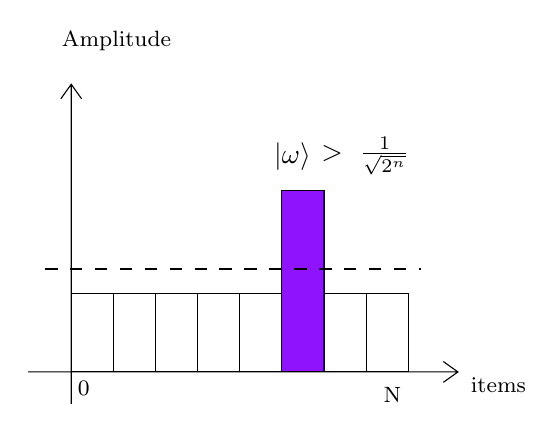
\begin{tikzpicture}[x=0.75pt,y=0.75pt,yscale=-1,xscale=1]
      %uncomment if require: \path (0,421); %set diagram left start at 0, and has height of 421

      %Shape: Axis 2D [id:dp9734077209252769] 
      \draw  (390,249.6) -- (597,249.6)(410.7,111) -- (410.7,265) (590,244.6) -- (597,249.6) -- (590,254.6) (405.7,118) -- (410.7,111) -- (415.7,118)  ;
      %Shape: Rectangle [id:dp3704883525061837] 
      \draw   (410.7,211.67) -- (431,211.67) -- (431,249.6) -- (410.7,249.6) -- cycle ;
      %Shape: Rectangle [id:dp044532975443389855] 
      \draw   (431,211.67) -- (451.3,211.67) -- (451.3,249.6) -- (431,249.6) -- cycle ;
      %Shape: Rectangle [id:dp7877425682227512] 
      \draw   (451.3,211.67) -- (471.6,211.67) -- (471.6,249.6) -- (451.3,249.6) -- cycle ;
      %Shape: Rectangle [id:dp9424861909526165] 
      \draw   (471.6,211.67) -- (491.9,211.67) -- (491.9,249.6) -- (471.6,249.6) -- cycle ;
      %Shape: Rectangle [id:dp22778928407890264] 
      \draw   (491.9,211.67) -- (512.2,211.67) -- (512.2,249.6) -- (491.9,249.6) -- cycle ;
      %Shape: Rectangle [id:dp5422997780895953] 
      \draw  [fill={rgb, 255:red, 144; green, 19; blue, 254 }  ,fill opacity=1 ] (512.2,249.6) -- (532.5,249.6) -- (532.5,162) -- (512.2,162) -- cycle ;
      %Shape: Rectangle [id:dp7263987108332439] 
      \draw   (532.5,211.67) -- (552.8,211.67) -- (552.8,249.6) -- (532.5,249.6) -- cycle ;
      %Shape: Rectangle [id:dp5179786757543001] 
      \draw   (552.8,211.67) -- (573.1,211.67) -- (573.1,249.6) -- (552.8,249.6) -- cycle ;
      %Straight Lines [id:da21954100641972407] 
      \draw  [dash pattern={on 4.5pt off 4.5pt}]  (398.13,200) -- (579.13,200) ;

      % Text Node
      \draw (405,84) node [anchor=north west][inner sep=0.75pt]   [align=left] {{\footnotesize Amplitude}};
      % Text Node
      \draw (412.7,252.6) node [anchor=north west][inner sep=0.75pt]   [align=left] {{\footnotesize 0}};
      % Text Node
      \draw (560,256) node [anchor=north west][inner sep=0.75pt]   [align=left] {{\footnotesize N}};
      % Text Node
      \draw (602,251) node [anchor=north west][inner sep=0.75pt]   [align=left] {{\footnotesize items}};
      % Text Node
      \draw (507.2,138.07) node [anchor=north west][inner sep=0.75pt]    {$\ket{\omega }$};
      % Text Node
      \draw (530,135) node [anchor=north west][inner sep=0.75pt]    {$ >\ \frac{1}{\sqrt{2^{n}}}$};

    \end{tikzpicture}
    \caption{\label{fig:grover_step_3b} Grover's Algorithm Step 3b}
  \end{subfigure}
  \caption{\label{fig:grover_step_3} Grover's Algorithm Step 3}
\end{figure}
\vspace{10mm}

\noindent
As indicated in Figure \ref{fig:grover_step_3a}, a diffusion operator $U_s$ is applied which results in a rotation of $\ket{s}$ by $2\theta$. 
\pagebreak


\begin{figure}
\begin{center}
      
    \tikzset{every picture/.style={line width=0.75pt}} %set default line width to 0.75pt        
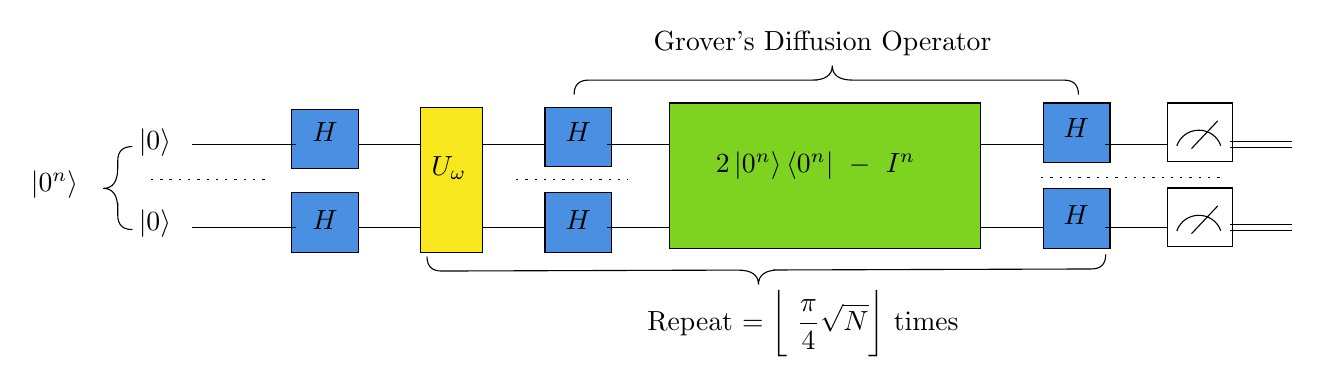
\begin{tikzpicture}[x=0.75pt,y=0.75pt,yscale=-1,xscale=1]
    %uncomment if require: \path (0,392); %set diagram left start at 0, and has height of 392

    %Shape: Rectangle [id:dp8937257723636158] 
    \draw  [fill={rgb, 255:red, 74; green, 144; blue, 226 }  ,fill opacity=1 ] (143,134) -- (175.19,134) -- (175.19,162.7) -- (143,162.7) -- cycle ;
    %Shape: Rectangle [id:dp007021083049765675] 
    \draw  [fill={rgb, 255:red, 74; green, 144; blue, 226 }  ,fill opacity=1 ] (143,174.3) -- (175.19,174.3) -- (175.19,203) -- (143,203) -- cycle ;
    %Shape: Rectangle [id:dp8911339020880464] 
    \draw  [fill={rgb, 255:red, 248; green, 231; blue, 28 }  ,fill opacity=1 ] (205,133) -- (235,133) -- (235,203) -- (205,203) -- cycle ;
    %Shape: Rectangle [id:dp25845825302570513] 
    \draw  [fill={rgb, 255:red, 74; green, 144; blue, 226 }  ,fill opacity=1 ] (265,133) -- (297.19,133) -- (297.19,161.7) -- (265,161.7) -- cycle ;
    %Shape: Rectangle [id:dp47274224679471666] 
    \draw  [fill={rgb, 255:red, 74; green, 144; blue, 226 }  ,fill opacity=1 ] (265,174.3) -- (297.19,174.3) -- (297.19,203) -- (265,203) -- cycle ;
    %Shape: Rectangle [id:dp5929473120919728] 
    \draw  [fill={rgb, 255:red, 126; green, 211; blue, 33 }  ,fill opacity=1 ] (325,131) -- (475,131) -- (475,201) -- (325,201) -- cycle ;
    %Shape: Rectangle [id:dp561230971836093] 
    \draw  [fill={rgb, 255:red, 74; green, 144; blue, 226 }  ,fill opacity=1 ] (505,131) -- (537.19,131) -- (537.19,159.7) -- (505,159.7) -- cycle ;
    %Shape: Rectangle [id:dp551714500077588] 
    \draw  [fill={rgb, 255:red, 74; green, 144; blue, 226 }  ,fill opacity=1 ] (505,172.3) -- (537.19,172.3) -- (537.19,201) -- (505,201) -- cycle ;
    %Shape: Rectangle [id:dp014371224119280157] 
    \draw   (565,131) -- (596.33,131) -- (596.33,159.22) -- (565,159.22) -- cycle ;
    %Shape: Arc [id:dp45728741367881365] 
    \draw  [draw opacity=0] (569.39,151.72) .. controls (570.82,147.31) and (575.03,144.13) .. (579.99,144.13) .. controls (584.9,144.13) and (589.07,147.24) .. (590.55,151.57) -- (579.99,155.06) -- cycle ; \draw   (569.39,151.72) .. controls (570.82,147.31) and (575.03,144.13) .. (579.99,144.13) .. controls (584.9,144.13) and (589.07,147.24) .. (590.55,151.57) ;  
    %Straight Lines [id:da3994764524189143] 
    \draw    (576.46,153) -- (589.1,139.61) ;
    %Shape: Rectangle [id:dp7321580418061253] 
    \draw   (565,172) -- (596.33,172) -- (596.33,200.22) -- (565,200.22) -- cycle ;
    %Shape: Arc [id:dp575518695312089] 
    \draw  [draw opacity=0] (569.39,192.72) .. controls (570.82,188.31) and (575.03,185.13) .. (579.99,185.13) .. controls (584.9,185.13) and (589.07,188.24) .. (590.55,192.57) -- (579.99,196.06) -- cycle ; \draw   (569.39,192.72) .. controls (570.82,188.31) and (575.03,185.13) .. (579.99,185.13) .. controls (584.9,185.13) and (589.07,188.24) .. (590.55,192.57) ;  
    %Straight Lines [id:da9653097238135147] 
    \draw    (576.46,194) -- (589.1,180.61) ;
    %Straight Lines [id:da054926584620969665] 
    \draw    (95,151) -- (145,151) ;
    %Straight Lines [id:da1998461114344101] 
    \draw    (95,191) -- (145,191) ;
    %Straight Lines [id:da13455039306792682] 
    \draw    (175,151) -- (205,151) ;
    %Straight Lines [id:da8941875904744676] 
    \draw    (175,191) -- (205,191) ;
    %Straight Lines [id:da16169269211888615] 
    \draw    (235,151) -- (265,151) ;
    %Straight Lines [id:da6385231938077083] 
    \draw    (235,191) -- (265,191) ;
    %Straight Lines [id:da21590920227006993] 
    \draw    (295,151) -- (325,151) ;
    %Straight Lines [id:da44624469722388915] 
    \draw    (295,191) -- (325,191) ;
    %Straight Lines [id:da9474262709127792] 
    \draw    (475,191) -- (505,191) ;
    %Straight Lines [id:da8304606265085992] 
    \draw    (475,151) -- (505,151) ;
    %Straight Lines [id:da4700710359224989] 
    \draw    (535,151) -- (565,151) ;
    %Straight Lines [id:da09738039485721028] 
    \draw    (535,191) -- (565,191) ;
    %Straight Lines [id:da7131108234298331] 
    \draw    (595,149.5) -- (625,149.5)(595,152.5) -- (625,152.5) ;
    %Straight Lines [id:da9226246067589841] 
    \draw    (595,189.5) -- (625,189.5)(595,192.5) -- (625,192.5) ;
    %Shape: Brace [id:dp5786954336630095] 
    \draw   (208.13,205) .. controls (208.15,209.67) and (210.49,211.99) .. (215.16,211.98) -- (357.81,211.53) .. controls (364.48,211.51) and (367.82,213.83) .. (367.83,218.5) .. controls (367.82,213.83) and (371.14,211.49) .. (377.81,211.47)(374.81,211.48) -- (528.16,210.99) .. controls (532.83,210.98) and (535.15,208.64) .. (535.13,203.97) ;
    %Shape: Brace [id:dp3814057437492582] 
\draw   (522,127) .. controls (522,122.33) and (519.67,120) .. (515,120) -- (413.38,120) .. controls (406.71,120) and (403.38,117.67) .. (403.38,113) .. controls (403.38,117.67) and (400.05,120) .. (393.38,120)(396.38,120) -- (286,120) .. controls (281.33,120) and (279,122.33) .. (279,127) ;
    %Shape: Brace [id:dp5248227356988384] 
    \draw   (66.13,152) .. controls (61.46,152) and (59.13,154.33) .. (59.13,159) -- (59.13,162.16) .. controls (59.13,168.83) and (56.8,172.16) .. (52.13,172.16) .. controls (56.8,172.16) and (59.13,175.49) .. (59.13,182.16)(59.13,179.16) -- (59.13,185) .. controls (59.13,189.67) and (61.46,192) .. (66.13,192) ;
    %Straight Lines [id:da6246903517915476] 
    \draw  [dash pattern={on 0.84pt off 2.51pt}]  (75.13,168) -- (133.13,168) ;
    %Straight Lines [id:da7651260164716407] 
    \draw  [dash pattern={on 0.84pt off 2.51pt}]  (251,168) -- (305.13,168) ;
    %Straight Lines [id:da5357419850229155] 
    \draw  [dash pattern={on 0.84pt off 2.51pt}]  (504,167) -- (592.13,167) ;

    % Text Node
    \draw (151.6,139.4) node [anchor=north west][inner sep=0.75pt]    {$H$};
    % Text Node
    \draw (151.6,181.4) node [anchor=north west][inner sep=0.75pt]    {$H$};
    % Text Node
    \draw (209,155.4) node [anchor=north west][inner sep=0.75pt]    {$U_{\omega }$};
    % Text Node
    \draw (273.6,139.4) node [anchor=north west][inner sep=0.75pt]    {$H$};
    % Text Node
    \draw (273.6,181.4) node [anchor=north west][inner sep=0.75pt]    {$H$};
    % Text Node
    \draw (513.6,137.4) node [anchor=north west][inner sep=0.75pt]    {$H$};
    % Text Node
    \draw (513.6,179.4) node [anchor=north west][inner sep=0.75pt]    {$H$};
    % Text Node
    \draw (346,153.4) node [anchor=north west][inner sep=0.75pt]    {$2\ket{0^{n}}\bra{0^{n}} \ -\ I^{n}$};
    % Text Node
    \draw (68,142.4) node [anchor=north west][inner sep=0.75pt]    {$\ket{0}$};
    % Text Node
    \draw (68,181.4) node [anchor=north west][inner sep=0.75pt]    {$\ket{0}$};
    % Text Node
    \draw (16,162.4) node [anchor=north west][inner sep=0.75pt]    {$\ket{0^{n}}$};
    % Text Node
    \draw (316,95) node [anchor=north west][inner sep=0.75pt]   [align=left] {Grover's Diffusion Operator};
    % Text Node
    \draw (313,220) node [anchor=north west][inner sep=0.75pt]   [align=left] {Repeat  $\displaystyle  = \bigg\lfloor \ \frac{\pi }{4}\sqrt{N} \bigg\rfloor$ times};

\end{tikzpicture}
\end{center}

  \caption{\label{fig:grover_circuit} Quantum circuit representation of Grover's Algorithm.}
\end{figure}

\vspace{5mm}


\noindent
The diffusion operator is expressed as:
\vspace{5mm}

\begin{equation}
U_s  = 2 \ket{s}\bra{s} - 1    
\end{equation}
\vspace{5mm}

\noindent
$U_s$ is a reflection at the hyperplane orthogonal to $\ket{\perp s}$  for vectors in the plane spanned by $\ket{s}$  and $\ket{\perp s}$, in other words a reflection about $\ket{s}$. 
\vspace{5mm}

\noindent
The product of two reflection operators $U_\omega$ and $U_s$ is a rotation in the plane spanned by $\ket{\omega}$ and $\ket{s'}$ through twice the angle $\theta$.
\vspace{5mm}

\noindent
By applying $U_s$ and $U_\omega$ the initial state $\ket{s}$ is rotated close to the state $\ket{\omega}$.
\vspace{5mm}

\noindent
After repeated Grover iterations, $\ket{s}$ approaches $\ket{\omega}$, at which point an observation in the computational basis
outputs a solution to the search problem with high probability.
\vspace{5mm}

\noindent
By looking at Figure \ref{fig:grover_step_3b}, the amplitude of $\ket{\omega}$ is reflected about the average amplitude. Referring to Figure \ref{fig:grover_step_2b}, the average amplitude is lowered below the dashed line and the reflection boosts the amplitude by about three times its original value, as depicted in Figure \ref{fig:grover_step_3b}.
\vspace{5mm}

\noindent
Step 2 and Step 3 will be repeated where necessary for $T$ times until the average amplitude approaches zero so that the amplitude for $\ket{\omega} \sim 1$\cite{de_wolf_main_nodate}.
\vspace{5mm}

\noindent
By observation, the number of times $T$ is required to apply the Grover's Algorithm according to Figure \ref{fig:grover_step_3a} can be written as:
\vspace{5mm}

\noindent
\begin{equation}
\theta_T = (2T + 1)\theta
\end{equation}

Where $\theta_T \approx \frac{\pi}{2}$ and $T$ is chosen to the nearest integer. 
\pagebreak

\noindent
For an unstructured search through a sufficiently large list, $\theta$ will be small. Using the small angle approximation, $\sin\theta \approx \theta$. 
\vspace{5mm}

\noindent
Recall that $\sin\theta = \frac{1}{\sqrt{2^n}}$
\vspace{5mm}

\noindent
Hence:
\vspace{5mm}

\noindent
\begin{equation}
T \approx \frac{\pi}{4\theta} \approx \frac{\pi}{4}\sqrt{2^n}    
\end{equation}

Note that $N = 2^n$ has been used interchangeably in this literature.
\vspace{5mm}

\noindent
Consequently, it is shown that $T$ is directly proportional to the order $O(\sqrt{N})$.
\vspace{5mm}

\noindent
In terms of the amplitude of the state $\ket{s}$, it is observed to grow linearly with the number of application of $\sim T\sqrt{N}$. Therefore the amplitude and the probability are both amplified in Grover's Algorithm.
\vspace{5mm}

\noindent
For multiple search entries $M$, the number of Grover's iteration would be roughly $\sqrt{\frac{N}{M}}$.
\vspace{10mm}

\subsection{Advantages and Disadvantages}
\vspace{5mm}

\noindent
The obvious advantage of the Grover's Algorithm is the quadratic speed up over classical search algorithms. 
\vspace{5mm}

\noindent
In the previous chapter, Grover's Algorithm shows amplitude amplification on the target state $\ket{\omega}$ and this can be used to speed up a wide variety of other algorithms\cite{noauthor_grovers_nodate}. 
\vspace{5mm}

\noindent
One of the few drawbacks of the Grover's Algorithm is that it is probabilistic. However the probability error can be significantly reduced by repeating the algorithm.
\vspace{5mm}

\noindent
Due to the constraints of currently available quantum computers, Grover's Algorithm is yet to yield any  meaningful quadratic speed up compared to classical algorithms\cite{noauthor_grovers_2022}.

\pagebreak
\section{Using Grover's Algorithm to solve Sudoku}

A quantum search algorithm that can search unstructured data sets in a significantly shorter time span than classical computational methods would be extremely useful and could be applied in a variety of ways. In this section we're going to demonstrate a very simple usage of Grover's Algorithm by showcasing how it could be implemented to solve a 2x2 Binary Sudoku Board. 

\setlength{\arrayrulewidth}{0.5mm}
\setlength{\tabcolsep}{18pt}
\renewcommand{\arraystretch}{1.5}
\begin{figure}[h]
\begin{center}
    

\begin{tabular}{ |c|c|c| } 
\hline
V0 & V1  \\ 
\hline
V2 & V3 \\ 
\hline
\end{tabular}
\end{center}
\caption{2x2 Sudoku Board with variables V0,..,V3 \in \{0, 1\}}
\label{fig:Sudoku Board}
\end{figure}

\subsection{Making the Oracle}\label{Making the Oracle 2x2}


For this Sudoku board there are three main rules to be aware of:
\begin{itemize}
    \item Each box can only be filled with a single number, either 0 or 1
    \item No column can contain two of the same number
    \item No row can contain two of the same number
\end{itemize}

Given that we are only dealing with a maximum of two number options (0 and 1) we can represent each variable $V\textsubscript{X}$ (where X $\in \{0, 1, 2, 3\}$) as a singular qubit which gives us 4 input qubits, this satisfies our first rule. 
Rules 2 and 3 state that no adjacent variables can be equal to each other, the way this is done is using an XOR gate over two qubits which represent adjacent variables. For example, $V\textsubscript{0}$ (XOR) $V\textsubscript{1}$ returns $\ket{0}$ when $V\textsubscript{0}$ = $V\textsubscript{1}$ but returns $\ket{1}$ when $V\textsubscript{0} \neq V\textsubscript{1}$. With 4 sets of comparisons to make, there is going to be a set of 4 XOR gates with the outputs for each XOR gate being stored in a separate qubit (which we'll refer to as condition qubits). This means that in total we have 8 qubits but to fully complete the Oracle gate we're going to need 1 more. After each comparison is stored in the 4 condition qubits we need to check that every condition qubit is in the state $\ket{1}$ (which is akin to saying every rule in the Sudoku board is obeyed); to do this a customised Control-Not gate is applied across each condition qubit (where the condition qubits are the control and the target/ return value is stored in the final 9th qubit which we'll refer to as the output qubit). The final step in creating the Oracle gate is resetting every value in the 4 condition qubits by reapplying every XOR gate.  
\\ \\
As shown in \ref{The Oracle}, the Oracle gate acts upon the circuit $\ket{x}$ such that:

\begin{equation}
\begin{cases}
      U_{\omega}\ket{x} = \ket{x}  & \text{for} \ x \neq \omega, \ f(x) = 0 \\
      U_{\omega}\ket{x} = -\ket{x}  & \text{for} \ x = \omega, \ f(x) =1 \\
\end{cases}  
\end{equation}

If we represent our circuit $\ket{x}$ as three registers; one being the 4 input qubits $\ket{V\textsubscript{X}}$, another being the 4 condition qubits $\ket{c}$ and the final register being the last output qubit $\ket{out}$ then the Oracle should act on our circuit like so:

\begin{equation}
\begin{cases}
      U_{\omega}\ket{V\textsubscript{X}}\ket{c}\ket{out} = \ket{V\textsubscript{X}}\ket{c}\ket{out}  & \text{for} \ V\textsubscript{X} \neq \omega, \ f(V\textsubscript{X}) = 0 \\
      U_{\omega}\ket{V\textsubscript{X}}\ket{c}\ket{out} = -\ket{V\textsubscript{X}}\ket{c}\ket{out}  & \text{for} \ V\textsubscript{X} = \omega, \ f(V\textsubscript{X}) =1 \\
       
\end{cases}  
\end{equation}

For our problem as described at the start of this section \ref{Making the Oracle 2x2}, the input qubits are only used as controls whilst the condition qubits are reset back to their former values; this means that the only register that is acted upon is $\ket{out}$ by combining the results of every XOR computation. This looks like:

\begin{equation}
\begin{cases}
      U_{\omega}\ket{V\textsubscript{X}}\ket{c}\ket{out} = \ket{V\textsubscript{X}}\ket{c}\ket{out \oplus f(V\textsubscript{X})}  & \text{for} \ V\textsubscript{X} \neq \omega, \ f(V\textsubscript{X}) = 0 \\
      U_{\omega}\ket{V\textsubscript{X}}\ket{c}\ket{out} = -\ket{V\textsubscript{X}}\ket{c}\ket{out \oplus f(V\textsubscript{X})}  & \text{for} \ V\textsubscript{X} = \omega, \ f(V\textsubscript{X}) =1 \\
    
\end{cases}  
\end{equation}
where $\oplus$ is the combined XOR operator over $\ket{V\textsubscript{X}}$ which is stored in $\ket{c}$.
\\

From this we can determine that $\ket{out}$ must be equal to the superposition state $\ket{-}$ = $\frac{1}{\sqrt{2}}(\ket{0} - \ket{1})$. 
\subsubsection{Case 1}
Looking at the case where f(V\textsubscript{X}) = 0:
\\
\begin{equation}
U_\omega\ket{V\textsubscript{X}\ket{c}\ket{-}} = \ket{V\textsubscript{X}\ket{c}\ket{- \oplus f(V\textsubscript{X})}} = \ket{V\textsubscript{X}}\ket{c} \otimes \frac{1}{\sqrt{2}}(\ket{0} \oplus f(V\textsubscript{X}) - \ket{1 \oplus f(V\textsubscript{X})}) 
\end{equation}

Remembering the rules for XOR gates, this can be simplified to:

\begin{equation}
U_\omega\ket{V\textsubscript{X}\ket{c}\ket{-}} = \ket{V\textsubscript{X}}\ket{c} \otimes \frac{1}{\sqrt{2}}(\ket{0} - \ket{1}) \\
= \ket{V\textsubscript{X}}\ket{c}\ket{-}
\end{equation}

\\
\subsubsection{Case 2}

Doing the same thing for the case where f(V\textsubscript{X}) = 1 (such that V\textsubscript{X} = $\omega$):

\begin{equation}
U_\omega\ket{V\textsubscript{X}\ket{c}\ket{-}} = \ket{V\textsubscript{X}}\ket{c} \otimes \frac{1}{\sqrt{2}}(\ket{0} \oplus f(V\textsubscript{X}) - \ket{1 \oplus f(V\textsubscript{X})})
\end{equation}

After applying the XOR gate, this simplifies to: 

\begin{equation}
\ket{V\textsubscript{X}}\ket{c} \otimes \frac{1}{\sqrt{2}}(\ket{0} \oplus f(V\textsubscript{X}) - \ket{1 \oplus f(V\textsubscript{X})}) = \ket{V\textsubscript{X}}\ket{c} \otimes \frac{1}{\sqrt{2}}(\ket{1} - \ket{0})
\end{equation}

This gives us that:

\begin{equation}
 U_\omega\ket{V\textsubscript{X}\ket{c}\ket{-}}= \ket{V\textsubscript{X}}\ket{c} \otimes \frac{1}{\sqrt{2}}(\ket{1} - \ket{0}) = - \ket{V\textsubscript{X}}\ket{c}\ket{-}
\end{equation}
\\
\\

So to recap, the Oracle gate is created by setting $\ket{out}$ to $\ket{-}$. Then by using a combination of XOR gates over $\ket{V\textsubscript{X}}$ and storing the values in $\ket{c}$ we can check whether each rule is observed. By using a Controlled-Not gate over $\ket{c}$ and storing the value in $\ket{out}$ the state we can apply a phase shift. Finally, the values in $\ket{c}$ are reset back to $\ket{0000}$ by reapplying all of the XOR gates.

\subsection{The Rest of the Circuit}
The Diffusion Operator works exactly as stated at the end of \ref{How the Algorithm Works} but instead of operating over every qubit, the Diffusion operator only works over $\ket{V\textsubscript{X}}$ as these are the only qubits that we hope to amplify. With Hadamards placed on the qubits in $\ket{V\textsubscript{X}}$ as shown in \ref{fig:grover_circuit}, we apply the Oracle and Diffusion Operators twice and then measure the states of $\ket{V\textsubscript{X}}$ to, hopefully, get our solution.


\pagebreak

\section{Phase Estimation}
\vspace{5mm}

\subsection{Introduction}
Suppose you have a unitary operator $U$ and its eigenvector $\ket{u}$ with eigenvalue $e^{2\pi i \phi}$, with $\phi$ unknown. By performing phase estimation, we can estimate $\phi$ (exact if the decimal expansion of $\phi$ is finite), up to required precision $n$. Phase estimation is needed for the algorithm of order-finding and it's extension, Shor's factoring algorithm. The figure below illustrate this process.

\vspace{5mm}
\begin{figure}[h]
    \centering
    

\tikzset{every picture/.style={line width=0.75pt}} %set default line width to 0.75pt        

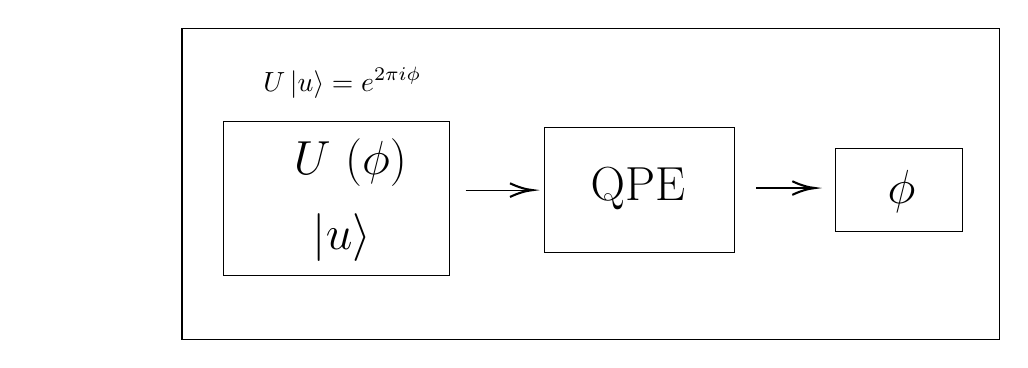
\begin{tikzpicture}[x=0.75pt,y=0.75pt,yscale=-1,xscale=1]
\path (0,195); %set diagram left start at 0, and has height of 300

%Shape: Rectangle [id:dp5239908419271088] 
\draw   (249,94) -- (340.33,94) -- (340.33,154) -- (249,154) -- cycle ;
%Shape: Rectangle [id:dp798673162776731] 
\draw   (94.33,91) -- (203.33,91) -- (203.33,165) -- (94.33,165) -- cycle ;
%Straight Lines [id:da0439097804330606] 
\draw    (211,124) -- (241.33,124) ;
\draw [shift={(243.33,124)}, rotate = 180] [color={rgb, 255:red, 0; green, 0; blue, 0 }  ][line width=0.75]    (10.93,-3.29) .. controls (6.95,-1.4) and (3.31,-0.3) .. (0,0) .. controls (3.31,0.3) and (6.95,1.4) .. (10.93,3.29)   ;
%Straight Lines [id:da053999006588390186] 
\draw    (351,123) -- (377.33,123) ;
\draw [shift={(379.33,123)}, rotate = 180] [color={rgb, 255:red, 0; green, 0; blue, 0 }  ][line width=0.75]    (10.93,-3.29) .. controls (6.95,-1.4) and (3.31,-0.3) .. (0,0) .. controls (3.31,0.3) and (6.95,1.4) .. (10.93,3.29)   ;
%Shape: Rectangle [id:dp5103744878863842] 
\draw   (389,104) -- (450.33,104) -- (450.33,144) -- (389,144) -- cycle ;
%Shape: Rectangle [id:dp6849328641759378] 
\draw   (74.33,46) -- (468.33,46) -- (468.33,196) -- (74.33,196) -- cycle ;

% Text Node
\draw (270,112) node [anchor=north west][inner sep=0.75pt]  [font=\LARGE] [align=left] {QPE};
% Text Node
\draw (127,98) node [anchor=north west][inner sep=0.75pt]   [align=left][font=\LARGE] {$\displaystyle U\ ( \phi )$};
% Text Node
\draw (112,63) node [anchor=north west][inner sep=1pt]   [align=left]{$\displaystyle U\ket{u} =e^{2\pi i\phi }$};
% Text Node
\draw (136,134) node [anchor=north west][inner sep=0.75pt] [font=\LARGE]  [align=left] {$\displaystyle \ket{u}$};
% Text Node
\draw (413,113) node [anchor=north west][inner sep=0.75pt][font=\LARGE]   [align=left] {$\displaystyle \phi $};


\end{tikzpicture}

\caption{Phase Estimation (abbreviated as QPE).}
\end{figure}

\subsection{Quantum Fourier Transform}
\vspace{5mm}

To implement the phase estimation algorithm, the key ingredient is the quantum Fourier transform. Quantum Fourier transform is analogous to the classical discrete Fourier transform, where the basis of a vector is changed into another basis that is useful for computation or analysis. The effect of quantum Fourier transform on an arbitrary state vector can be summarised as below \cite{nielsen_quantum_2010}:
\begin{equation}
    \ket{v} = \frac{1}{\sqrt{N}} \sum_{i=0}^{N-1}{x_i \ket{i}} \xRightarrow{QFT} \ket{\Tilde{v}} = \frac{1}{\sqrt{N}}\sum_{j=0}^{N-1} y_j \ket{j}
\end{equation} 

\noindent
Note that only the amplitudes of the eigenstates are affected by this transformation. Similar to Fourier transform which decomposes functions depending on space or time into functions depending on spatial frequency or temporal frequency, QFT maps the computational basis states between the $\hat{\textbf{z}}$-basis states to the $\hat{\textbf{x}}$-basis states.
\vspace{5mm}

\noindent
The $\hat{\textbf{x}}$-basis states are defined as:
\vspace{5mm}

\begin{equation}
\ket{+} = \frac{1}{\sqrt{2}}(\ket{0} + \ket{1}) \ \text{and} \ \ket{-} = \frac{1}{\sqrt{2}}(\ket{0} - \ket{1})   
\end{equation}

\pagebreak

\noindent
For multi-qubit states in the computational basis have corresponding states in the Fourier basis. The QFT is the function that transforms between these bases\cite{noauthor_quantum_nodate-1}:
\vspace{5mm}

\begin{equation}
\ket{\text{State in computational basis}} \rightarrow{\text{QFT}} \ket{\text{State in Fourier basis}}  
\end{equation}
\vspace{5mm}

\qquad $\text{QFT}\ket{x} = \ket{\tilde{x}}$
\vspace{5mm}

For a $n$ qubit states, the QFT has the effect of \cite{nielsen_quantum_2010}:
\vspace{5mm}
\begin{equation}
\text{QFT}_N\ket{x} = \frac{1}{\sqrt{N}} \sum\limits_{y=0}^{N-1}e^{2i\pi\frac{xy}{2^n}}\ket{y} \ , \ \text{for} \ N = 2^n    
\end{equation}

\vspace{5mm}

\begin{equation}
=  \frac{1}{\sqrt{N}} \sum\limits_{y=0}^{N-1}e^{2i\pi x(\sum_{k=1}^{n}\frac{y_k}{2^k})}\ket{y...y_n} 
\end{equation}
\vspace{5mm}

Rewriting $y$ in binary fraction $y= y_1 ... y_n, \ \frac{y}{2^n} = \sum\limits_{k=1}^{n}\frac{y_k}{2^k}$   
\vspace{5mm}

\begin{equation}
= \frac{1}{\sqrt{N}} \sum\limits_{y=0}^{N-1}\prod\limits_{k=1}^{n}e^{2i\pi x\frac{y_k}{2^k}}\ket{y...y_n}    
\end{equation}
\vspace{5mm}

\noindent
After expanding the exponential of a sum to a product of exponentials.
\vspace{5mm}

\begin{equation}
= \frac{1}{\sqrt{N}}\bigotimes\limits_{k=1}^{n}(\ket{0} + e^{\frac{2i\pi x}{2^k}}\ket{1})  
\end{equation}
\vspace{5mm}

\noindent
After rearranging the sum and products, and expanding $\sum\limits_{y=0}^{N-1} = \sum\limits_{y_1=0}^{1}\sum\limits_{y_2=0}^{1}...\sum\limits_{y_0=0}^{1} $
\vspace{5mm}

\begin{equation}
= \frac{1}{\sqrt{N}}(\ket{0} + e^{\frac{2i\pi x}{2}}\ket{1}) \otimes (\ket{0} + e^{\frac{2i\pi x}{2^2}}\ket{1}) \otimes ... \otimes(\ket{0} + e^{\frac{2i\pi x}{2^{n-1}}}\ket{1}) \otimes (\ket{0} + e^{\frac{2i\pi x}{2^n}}\ket{1})    
\end{equation}
\pagebreak

The circuit to implement QFT for a n-qubit state is shown below
\vspace{5mm}

\noindent


\begin{figure}[h]
    \centering


\tikzset{every picture/.style={line width=0.75pt}} %set default line width to 0.75pt        

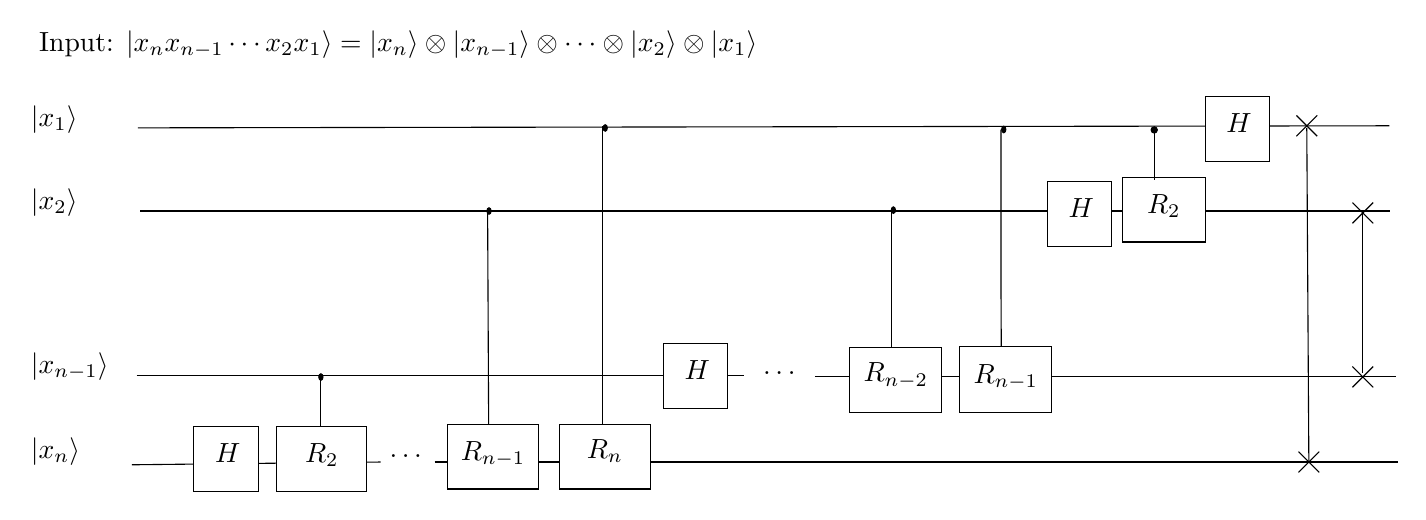
\begin{tikzpicture}[x=0.75pt,y=0.75pt,yscale=-1,xscale=1]
%uncomment if require: \path (0,300); %set diagram left start at 0, and has height of 300

%Straight Lines [id:da3967690953518057] 
\draw    (380,179) -- (659.75,179) ;
%Straight Lines [id:da9878029252695806] 
\draw    (469.83,168.25) -- (469.69,139.19) -- (469.69,59.8) ;
%Straight Lines [id:da8582177199826221] 
\draw    (416.83,168) -- (416.83,99.2) ;
%Straight Lines [id:da3196026977221085] 
\draw    (196.83,220) -- (660.75,220) ;
%Straight Lines [id:da07684763739566802] 
\draw    (50.88,221.33) -- (170.83,220) ;
%Shape: Rectangle [id:dp7166077461715553] 
\draw  [fill={rgb, 255:red, 255; green, 255; blue, 255 }  ,fill opacity=1 ] (80.83,203) -- (111.86,203) -- (111.86,234) -- (80.83,234) -- cycle ;

%Shape: Rectangle [id:dp758880806339667] 
\draw  [fill={rgb, 255:red, 255; green, 255; blue, 255 }  ,fill opacity=1 ] (120.83,203) -- (163.83,203) -- (163.83,234) -- (120.83,234) -- cycle ;

%Straight Lines [id:da9072316210568465] 
\draw    (141.83,203) -- (141.83,178.06) ;
%Shape: Rectangle [id:dp887638468970721] 
\draw  [fill={rgb, 255:red, 255; green, 255; blue, 255 }  ,fill opacity=1 ] (202.83,202) -- (246.83,202) -- (246.83,233) -- (202.83,233) -- cycle ;
%Straight Lines [id:da4039836031001398] 
\draw    (222.83,202) -- (222.33,99.5) ;
%Shape: Ellipse [id:dp5470892460263189] 
\draw  [fill={rgb, 255:red, 2; green, 2; blue, 2 }  ,fill opacity=1 ] (222,99.06) .. controls (222,99.92) and (222.45,100.62) .. (223,100.62) .. controls (223.55,100.62) and (224,99.92) .. (224,99.06) .. controls (224,98.2) and (223.55,97.5) .. (223,97.5) .. controls (222.45,97.5) and (222,98.2) .. (222,99.06) -- cycle ;

%Shape: Rectangle [id:dp7396779533097696] 
\draw  [fill={rgb, 255:red, 255; green, 255; blue, 255 }  ,fill opacity=1 ] (256.83,202) -- (300.83,202) -- (300.83,233) -- (256.83,233) -- cycle ;
%Straight Lines [id:da9953579128910641] 
\draw    (277.83,202) -- (277.83,58.33) ;
%Straight Lines [id:da304584348508544] 
\draw    (53.18,178.5) -- (217.35,178.5) -- (345.75,178.5) ;
%Straight Lines [id:da19441753788178195] 
\draw    (54.95,99.06) -- (222,99.06) -- (656.95,99.06) ;
%Straight Lines [id:da5686077293635534] 
\draw    (53.83,59) -- (656.83,58) ;
%Shape: Ellipse [id:dp6678818886024199] 
\draw  [fill={rgb, 255:red, 2; green, 2; blue, 2 }  ,fill opacity=1 ] (141,179.06) .. controls (141,179.92) and (141.45,180.62) .. (142,180.62) .. controls (142.55,180.62) and (143,179.92) .. (143,179.06) .. controls (143,178.2) and (142.55,177.5) .. (142,177.5) .. controls (141.45,177.5) and (141,178.2) .. (141,179.06) -- cycle ;
%Shape: Ellipse [id:dp7348740438597149] 
\draw  [fill={rgb, 255:red, 2; green, 2; blue, 2 }  ,fill opacity=1 ] (278,59.06) .. controls (278,59.92) and (278.45,60.62) .. (279,60.62) .. controls (279.55,60.62) and (280,59.92) .. (280,59.06) .. controls (280,58.2) and (279.55,57.5) .. (279,57.5) .. controls (278.45,57.5) and (278,58.2) .. (278,59.06) -- cycle ;
%Shape: Rectangle [id:dp6251794280116343] 
\draw  [fill={rgb, 255:red, 255; green, 255; blue, 255 }  ,fill opacity=1 ] (307,163) -- (338.03,163) -- (338.03,194) -- (307,194) -- cycle ;

%Straight Lines [id:da48501832285910107] 
\draw    (617,59) -- (618,220) ;
%Straight Lines [id:da3619533645667148] 
\draw    (612,53) -- (622,63) ;
%Straight Lines [id:da1136318355264534] 
\draw    (622,53) -- (612,63) ;

%Straight Lines [id:da8858890162256563] 
\draw    (613,215) -- (623,225) ;
%Straight Lines [id:da6829327205842372] 
\draw    (623,215) -- (613,225) ;


%Straight Lines [id:da8840707107750161] 
\draw    (644,100) -- (644,177) ;
%Straight Lines [id:da454844448542837] 
\draw    (639,174) -- (649,184) ;
%Straight Lines [id:da7602550013601753] 
\draw    (649,174) -- (639,184) ;

%Straight Lines [id:da9458589943076327] 
\draw    (639,95) -- (649,105) ;
%Straight Lines [id:da01796925917370651] 
\draw    (649,95) -- (639,105) ;


%Shape: Rectangle [id:dp4590967975075022] 
\draw  [fill={rgb, 255:red, 255; green, 255; blue, 255 }  ,fill opacity=1 ] (449.83,164.25) -- (493.83,164.25) -- (493.83,196) -- (449.83,196) -- cycle ;
%Shape: Ellipse [id:dp4611610254403936] 
\draw  [fill={rgb, 255:red, 2; green, 2; blue, 2 }  ,fill opacity=1 ] (470,59.8) .. controls (470,60.68) and (470.45,61.39) .. (471,61.39) .. controls (471.55,61.39) and (472,60.68) .. (472,59.8) .. controls (472,58.91) and (471.55,58.2) .. (471,58.2) .. controls (470.45,58.2) and (470,58.91) .. (470,59.8) -- cycle ;
%Shape: Rectangle [id:dp47171557119826113] 
\draw  [fill={rgb, 255:red, 255; green, 255; blue, 255 }  ,fill opacity=1 ] (396.83,165) -- (440.83,165) -- (440.83,196) -- (396.83,196) -- cycle ;
%Shape: Ellipse [id:dp39067266570391845] 
\draw  [fill={rgb, 255:red, 2; green, 2; blue, 2 }  ,fill opacity=1 ] (416.83,98.64) .. controls (416.83,99.5) and (417.28,100.2) .. (417.83,100.2) .. controls (418.39,100.2) and (418.83,99.5) .. (418.83,98.64) .. controls (418.83,97.78) and (418.39,97.08) .. (417.83,97.08) .. controls (417.28,97.08) and (416.83,97.78) .. (416.83,98.64) -- cycle ;
%Shape: Rectangle [id:dp7816137489930797] 
\draw  [fill={rgb, 255:red, 255; green, 255; blue, 255 }  ,fill opacity=1 ] (491.97,85) -- (523,85) -- (523,116) -- (491.97,116) -- cycle ;

%Shape: Rectangle [id:dp8241920393207232] 
\draw  [fill={rgb, 255:red, 255; green, 255; blue, 255 }  ,fill opacity=1 ] (528,83) -- (568,83) -- (568,114) -- (528,114) -- cycle ;

%Straight Lines [id:da24945250453126844] 
\draw    (543.5,84) -- (543.5,60) ;
%Shape: Circle [id:dp18896475231461685] 
\draw  [fill={rgb, 255:red, 2; green, 2; blue, 2 }  ,fill opacity=1 ] (542,60) .. controls (542,60.83) and (542.67,61.5) .. (543.5,61.5) .. controls (544.33,61.5) and (545,60.83) .. (545,60) .. controls (545,59.17) and (544.33,58.5) .. (543.5,58.5) .. controls (542.67,58.5) and (542,59.17) .. (542,60) -- cycle ;


%Shape: Rectangle [id:dp7852662448600767] 
\draw  [fill={rgb, 255:red, 255; green, 255; blue, 255 }  ,fill opacity=1 ] (568,44) -- (599.03,44) -- (599.03,75) -- (568,75) -- cycle ;


% Text Node
\draw (1,47) node [anchor=north west][inner sep=0.75pt]   [align=left] {$\displaystyle \ket{x_{1}}$};
% Text Node
\draw (1,87) node [anchor=north west][inner sep=0.75pt]   [align=left] {$\displaystyle \ket{x_{2}}$};
% Text Node
\draw (1,166) node [anchor=north west][inner sep=0.75pt]   [align=left] {$\displaystyle \ket{x_{n-1}}$};
% Text Node
\draw (1,207) node [anchor=north west][inner sep=0.75pt]   [align=left] {$\displaystyle \ket{x_{n}}$};
% Text Node
\draw (5,11) node [anchor=north west][inner sep=0.75pt]   [align=left] {Input: $\displaystyle \ket{x_{n} x_{n-1} \cdots x_{2} x_{1}} =\ket{x_{n}} \otimes \ket{x_{n-1}} \otimes \cdots \otimes \ket{x_{2}} \otimes \ket{x_{1}}$};
% Text Node
\draw (173.83,215) node [anchor=north west][inner sep=0.75pt]   [align=left] {$\displaystyle \dotsc $};
% Text Node
\draw (268.83,208) node [anchor=north west][inner sep=0.75pt]   [align=left] {$\displaystyle R_{n}$};
% Text Node
\draw (133.19,210) node [anchor=north west][inner sep=0.75pt]   [align=left] {$\displaystyle R_{2}$};
% Text Node
\draw (89.83,209.7) node [anchor=north west][inner sep=0.75pt]   [align=left] {$\displaystyle H$};
% Text Node
\draw (316,169.7) node [anchor=north west][inner sep=0.75pt]   [align=left] {$\displaystyle H$};
% Text Node
\draw (208.23,209) node [anchor=north west][inner sep=0.75pt]   [align=left] {$\displaystyle R_{n-1}$};
% Text Node
\draw (402.23,171) node [anchor=north west][inner sep=0.75pt]   [align=left] {$\displaystyle R_{n-2}$};
% Text Node
\draw (353.83,175) node [anchor=north west][inner sep=0.75pt]   [align=left] {$\displaystyle \dotsc $};
% Text Node
\draw (455.23,171.63) node [anchor=north west][inner sep=0.75pt]   [align=left] {$\displaystyle R_{n-1}$};
% Text Node
\draw (500.97,91.7) node [anchor=north west][inner sep=0.75pt]   [align=left] {$\displaystyle H$};
% Text Node
\draw (538.8,90) node [anchor=north west][inner sep=0.75pt]   [align=left] {$\displaystyle R_{2}$};
% Text Node
\draw (577,50.7) node [anchor=north west][inner sep=0.75pt]   [align=left] {$\displaystyle H$};


\end{tikzpicture}

\caption{The QFT Circuit}
\end{figure}
\vspace{5mm}

where $H$ is the Hadamard gate, \(R_n = 
\begin{bmatrix}
    1 & 0 \\
    0 & e^{2\pi i/2^k}
\end{bmatrix} \)
, and the 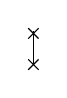
\begin{tikzpicture}[x=0.75pt,y=0.75pt,yscale=0.5,xscale=0.5]
%uncomment if require: \path (0,300); %set diagram left start at 0, and has height of 300

%Straight Lines [id:da5239484844882938] 
\draw    (85,16) -- (85,47) ;
%Straight Lines [id:da8400020556735358] 
\draw    (80,40) -- (90,50) ;
%Straight Lines [id:da24481923694858] 
\draw    (90,40) -- (80,50) ;

%Straight Lines [id:da0676093949143659] 
\draw    (80,10) -- (90,20) ;
%Straight Lines [id:da9539947353268269] 
\draw    (90,10) -- (80,20) ;
\end{tikzpicture} is a swap gate, which swaps the qubit i with the n-i qubit. However, the phase estimation algorithm requires the inverse QFT, which is easy to construct by flipping the circuit horizontally, and conjugate the phases in the $R_k$ gate.
\pagebreak
\subsection{The Algorithm}
The phase estimation procedure uses two registers, with the first register containing $m$ qubits (all in the state $\ket{0}$) and the second register is in the state $\ket{u}$, and contains as many qubits as required for $\ket{u}$. The number of qubits $m$ for first register is dependent on the precision of the phase required, which will be discussed in the next section. The algorithm can be summarized below:
\begin{enumerate}
    \item Hadamard gates are applied to all qubits in first register.
    \item Control-U gates raised to successive powers of two is applied consecutively to the second register, with the controls covering the first qubit to the last qubit in the first register.
    \item The inverse QFT operation is then applied on the first register to obtain a number, which needs further to be further divided by $2^m$ to recover the estimation of the phase.
\end{enumerate}
The circuit below sums up the whole procedure.
\vspace{5mm}


    
\begin{figure}[h]

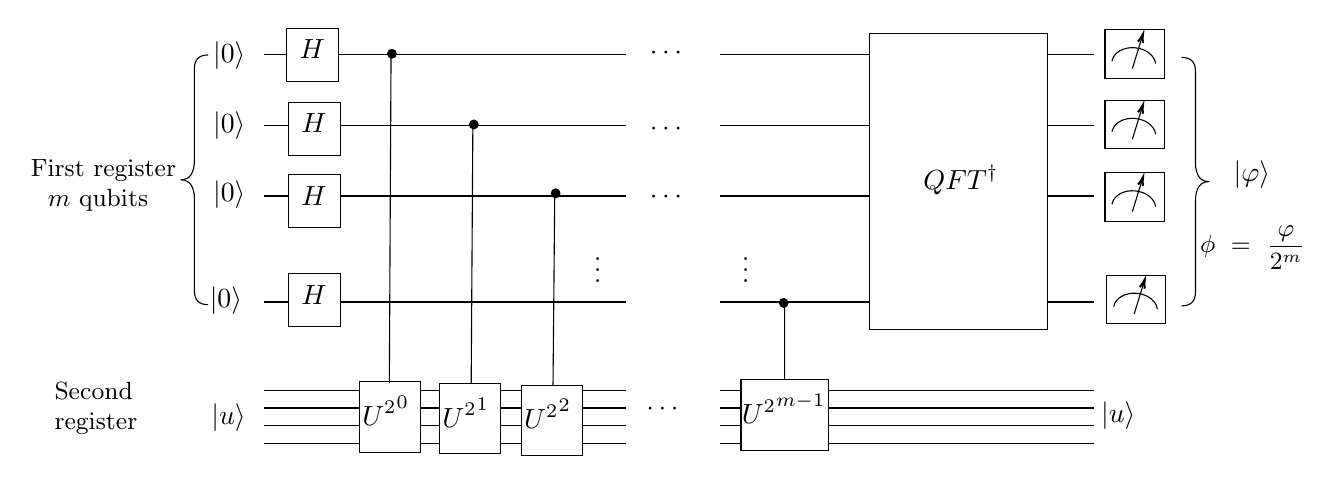
\begin{tikzpicture}[x=0.75pt,y=0.75pt,yscale=-0.95,xscale=0.95]
%uncomment if require: \path (0,255); %set diagram left start at 0, and has height of 255

%Straight Lines [id:da9194835056551176] 
\draw    (120.56,38.44) -- (304.21,38.44) ;
%Straight Lines [id:da6985548639030699] 
\draw    (120.56,74.27) -- (304.21,74.27) ;
%Straight Lines [id:da7116263330867054] 
\draw    (120.56,110.11) -- (304.21,110.11) ;
%Straight Lines [id:da8626589126730531] 
\draw    (120.56,163.86) -- (304.21,163.86) ;
%Straight Lines [id:da19695588367886063] 
\draw    (120.56,208.65) -- (304.21,208.65) ;
%Straight Lines [id:da10938435456147] 
\draw    (120.56,217.61) -- (304.21,217.61) ;
%Straight Lines [id:da4912942246519334] 
\draw    (120.56,226.57) -- (304.21,226.57) ;
%Straight Lines [id:da12940095959327003] 
\draw    (120.56,235.53) -- (304.21,235.53) ;
%Shape: Rectangle [id:dp15884195779468213] 
\draw  [fill={rgb, 255:red, 255; green, 255; blue, 255 }  ,fill opacity=1 ] (132.04,25) -- (158.54,25) -- (158.54,51.88) -- (132.04,51.88) -- cycle ;

%Shape: Rectangle [id:dp23256435967097955] 
\draw  [fill={rgb, 255:red, 255; green, 255; blue, 255 }  ,fill opacity=1 ] (132.93,62.63) -- (159.42,62.63) -- (159.42,89.5) -- (132.93,89.5) -- cycle ;

%Shape: Rectangle [id:dp37562370103024234] 
\draw  [fill={rgb, 255:red, 255; green, 255; blue, 255 }  ,fill opacity=1 ] (132.93,99.36) -- (159.42,99.36) -- (159.42,126.23) -- (132.93,126.23) -- cycle ;

%Shape: Rectangle [id:dp03136015448302287] 
\draw  [fill={rgb, 255:red, 255; green, 255; blue, 255 }  ,fill opacity=1 ] (132.93,149.53) -- (159.42,149.53) -- (159.42,176.4) -- (132.93,176.4) -- cycle ;

%Shape: Rectangle [id:dp03155077547529872] 
\draw  [fill={rgb, 255:red, 255; green, 255; blue, 255 }  ,fill opacity=1 ] (169.1,204.17) -- (200.01,204.17) -- (200.01,240.01) -- (169.1,240.01) -- cycle ;

%Shape: Rectangle [id:dp9729186752169825] 
\draw  [fill={rgb, 255:red, 255; green, 255; blue, 255 }  ,fill opacity=1 ] (209.72,205.07) -- (240.63,205.07) -- (240.63,240.9) -- (209.72,240.9) -- cycle ;
%Shape: Rectangle [id:dp19964985396092239] 
\draw  [fill={rgb, 255:red, 255; green, 255; blue, 255 }  ,fill opacity=1 ] (251.23,205.97) -- (282.14,205.97) -- (282.14,241.8) -- (251.23,241.8) -- cycle ;
%Straight Lines [id:da7109063051521263] 
\draw    (351.93,38.44) -- (541.76,38.44) ;
%Straight Lines [id:da1930170699837772] 
\draw    (351.93,74.27) -- (541.76,74.27) ;
%Straight Lines [id:da7712890300467412] 
\draw    (351.93,110.11) -- (541.76,110.11) ;
%Straight Lines [id:da00469730483476738] 
\draw    (351.93,163.86) -- (541.76,163.86) ;
%Straight Lines [id:da9060427595505647] 
\draw    (351.93,208.65) -- (541.76,208.65) ;
%Straight Lines [id:da24660499214292575] 
\draw    (351.93,217.61) -- (541.76,217.61) ;
%Straight Lines [id:da8073093108188725] 
\draw    (351.93,226.57) -- (541.76,226.57) ;
%Straight Lines [id:da9156311780855882] 
\draw    (351.93,235.53) -- (541.76,235.53) ;
%Shape: Rectangle [id:dp5274524103344703] 
\draw  [fill={rgb, 255:red, 255; green, 255; blue, 255 }  ,fill opacity=1 ] (362.5,203.28) -- (406.65,203.28) -- (406.65,239.11) -- (362.5,239.11) -- cycle ;
%Straight Lines [id:da03444841972411539] 
\draw    (185,39.15) -- (184.14,205.07) ;
%Straight Lines [id:da009404546254211943] 
\draw    (226.5,74.09) -- (225.65,205.07) ;
%Straight Lines [id:da374044199582911] 
\draw    (268.01,110.82) -- (267.15,205.97) ;
%Straight Lines [id:da6555871247561469] 
\draw    (384.57,163.68) -- (384.6,203.28) ;
%Shape: Ellipse [id:dp31242914795993315] 
\draw  [fill={rgb, 255:red, 0; green, 0; blue, 0 }  ,fill opacity=1 ] (183.26,37.98) .. controls (183.26,36.75) and (184.24,35.75) .. (185.45,35.75) .. controls (186.67,35.75) and (187.65,36.75) .. (187.65,37.98) .. controls (187.65,39.2) and (186.67,40.2) .. (185.45,40.2) .. controls (184.24,40.2) and (183.26,39.2) .. (183.26,37.98) -- cycle ;
%Shape: Ellipse [id:dp8473767958403672] 
\draw  [fill={rgb, 255:red, 0; green, 0; blue, 0 }  ,fill opacity=1 ] (224.77,73.81) .. controls (224.77,72.58) and (225.75,71.59) .. (226.96,71.59) .. controls (228.17,71.59) and (229.15,72.58) .. (229.15,73.81) .. controls (229.15,75.04) and (228.17,76.03) .. (226.96,76.03) .. controls (225.75,76.03) and (224.77,75.04) .. (224.77,73.81) -- cycle ;
%Shape: Ellipse [id:dp8148369515275169] 
\draw  [fill={rgb, 255:red, 0; green, 0; blue, 0 }  ,fill opacity=1 ] (266.27,108.75) .. controls (266.27,107.52) and (267.25,106.52) .. (268.46,106.52) .. controls (269.67,106.52) and (270.66,107.52) .. (270.66,108.75) .. controls (270.66,109.98) and (269.67,110.97) .. (268.46,110.97) .. controls (267.25,110.97) and (266.27,109.98) .. (266.27,108.75) -- cycle ;
%Shape: Ellipse [id:dp35408407729589786] 
\draw  [fill={rgb, 255:red, 0; green, 0; blue, 0 }  ,fill opacity=1 ] (381.95,164.29) .. controls (381.95,163.06) and (382.94,162.07) .. (384.15,162.07) .. controls (385.36,162.07) and (386.34,163.06) .. (386.34,164.29) .. controls (386.34,165.52) and (385.36,166.52) .. (384.15,166.52) .. controls (382.94,166.52) and (381.95,165.52) .. (381.95,164.29) -- cycle ;
%Shape: Rectangle [id:dp08709255028482066] 
\draw  [fill={rgb, 255:red, 255; green, 255; blue, 255 }  ,fill opacity=1 ] (427.87,27.69) -- (517.92,27.69) -- (517.92,178.01) -- (427.87,178.01) -- cycle ;
%Shape: Rectangle [id:dp5816935501240186] 
\draw   (547.09,25.72) -- (577.08,25.72) -- (577.08,50.35) -- (547.09,50.35) -- cycle ;
%Shape: Arc [id:dp9020959249791546] 
\draw  [draw opacity=0] (550.64,41.69) .. controls (551.36,37.36) and (556.49,34.36) .. (562.41,34.91) .. controls (567.93,35.44) and (572.26,38.89) .. (572.77,42.92) -- (561.69,43.23) -- cycle ; \draw   (550.64,41.69) .. controls (551.36,37.36) and (556.49,34.36) .. (562.41,34.91) .. controls (567.93,35.44) and (572.26,38.89) .. (572.77,42.92) ;  
%Straight Lines [id:da9091015813949274] 
\draw    (560.97,45.47) -- (565.77,29.87) ;
\draw [shift={(566.36,27.96)}, rotate = 107.1] [color={rgb, 255:red, 0; green, 0; blue, 0 }  ][line width=0.75]    (4.37,-1.32) .. controls (2.78,-0.56) and (1.32,-0.12) .. (0,0) .. controls (1.32,0.12) and (2.78,0.56) .. (4.37,1.32)   ;

%Shape: Rectangle [id:dp715253231601205] 
\draw   (547.09,61.55) -- (577.08,61.55) -- (577.08,86.19) -- (547.09,86.19) -- cycle ;
%Shape: Arc [id:dp37902783293727893] 
\draw  [draw opacity=0] (550.64,77.53) .. controls (551.36,73.19) and (556.49,70.19) .. (562.41,70.75) .. controls (567.93,71.27) and (572.26,74.72) .. (572.77,78.76) -- (561.69,79.06) -- cycle ; \draw   (550.64,77.53) .. controls (551.36,73.19) and (556.49,70.19) .. (562.41,70.75) .. controls (567.93,71.27) and (572.26,74.72) .. (572.77,78.76) ;  
%Straight Lines [id:da6659199046761912] 
\draw    (560.97,81.3) -- (565.77,65.7) ;
\draw [shift={(566.36,63.79)}, rotate = 107.1] [color={rgb, 255:red, 0; green, 0; blue, 0 }  ][line width=0.75]    (4.37,-1.32) .. controls (2.78,-0.56) and (1.32,-0.12) .. (0,0) .. controls (1.32,0.12) and (2.78,0.56) .. (4.37,1.32)   ;

%Shape: Rectangle [id:dp5396491521682578] 
\draw   (547.09,98.28) -- (577.08,98.28) -- (577.08,122.92) -- (547.09,122.92) -- cycle ;
%Shape: Arc [id:dp19388376844570432] 
\draw  [draw opacity=0] (550.64,114.26) .. controls (551.36,109.92) and (556.49,106.92) .. (562.41,107.48) .. controls (567.93,108) and (572.26,111.45) .. (572.77,115.49) -- (561.69,115.79) -- cycle ; \draw   (550.64,114.26) .. controls (551.36,109.92) and (556.49,106.92) .. (562.41,107.48) .. controls (567.93,108) and (572.26,111.45) .. (572.77,115.49) ;  
%Straight Lines [id:da8381741578506972] 
\draw    (560.97,118.03) -- (565.77,102.43) ;
\draw [shift={(566.36,100.52)}, rotate = 107.1] [color={rgb, 255:red, 0; green, 0; blue, 0 }  ][line width=0.75]    (4.37,-1.32) .. controls (2.78,-0.56) and (1.32,-0.12) .. (0,0) .. controls (1.32,0.12) and (2.78,0.56) .. (4.37,1.32)   ;

%Shape: Rectangle [id:dp04173030496706942] 
\draw   (547.97,150.24) -- (577.97,150.24) -- (577.97,174.88) -- (547.97,174.88) -- cycle ;
%Shape: Arc [id:dp5223668572095267] 
\draw  [draw opacity=0] (551.52,166.22) .. controls (552.24,161.88) and (557.38,158.88) .. (563.29,159.44) .. controls (568.82,159.96) and (573.14,163.41) .. (573.65,167.45) -- (562.57,167.76) -- cycle ; \draw   (551.52,166.22) .. controls (552.24,161.88) and (557.38,158.88) .. (563.29,159.44) .. controls (568.82,159.96) and (573.14,163.41) .. (573.65,167.45) ;  
%Straight Lines [id:da3372443183558913] 
\draw    (561.86,169.99) -- (566.66,154.39) ;
\draw [shift={(567.25,152.48)}, rotate = 107.1] [color={rgb, 255:red, 0; green, 0; blue, 0 }  ][line width=0.75]    (4.37,-1.32) .. controls (2.78,-0.56) and (1.32,-0.12) .. (0,0) .. controls (1.32,0.12) and (2.78,0.56) .. (4.37,1.32)   ;

%Shape: Brace [id:dp8116415853490204] 
\draw   (92.27,38.55) .. controls (87.6,38.55) and (85.27,40.88) .. (85.27,45.55) -- (85.27,91.88) .. controls (85.27,98.55) and (82.94,101.88) .. (78.27,101.88) .. controls (82.94,101.88) and (85.27,105.21) .. (85.27,111.88)(85.27,108.88) -- (85.27,158.21) .. controls (85.27,162.88) and (87.6,165.21) .. (92.27,165.21) ;
%Shape: Brace [id:dp33774914340487494] 
\draw   (585.97,165.8) .. controls (590.64,165.8) and (592.97,163.47) .. (592.97,158.8) -- (592.97,112.8) .. controls (592.97,106.13) and (595.3,102.8) .. (599.97,102.8) .. controls (595.3,102.8) and (592.97,99.47) .. (592.97,92.8)(592.97,95.8) -- (592.97,46.8) .. controls (592.97,42.13) and (590.64,39.8) .. (585.97,39.8) ;

% Text Node
\draw (93.49,30.39) node [anchor=north west][inner sep=0.75pt]   [align=left] {$\displaystyle \ket{0}$};
% Text Node
\draw (93.49,66.22) node [anchor=north west][inner sep=0.75pt]   [align=left] {$\displaystyle \ket{0}$};
% Text Node
\draw (93.49,101.16) node [anchor=north west][inner sep=0.75pt]   [align=left] {$\displaystyle \ket{0}$};
% Text Node
\draw (91.73,154.91) node [anchor=north west][inner sep=0.75pt]   [align=left] {$\displaystyle \ket{0}$};
% Text Node
\draw (92.55,214.04) node [anchor=north west][inner sep=0.75pt]   [align=left] {$\displaystyle \ket{u}$};
% Text Node
\draw (137.35,29.49) node [anchor=north west][inner sep=0.75pt]   [align=left] {$\displaystyle H$};
% Text Node
\draw (138.23,67.12) node [anchor=north west][inner sep=0.75pt]   [align=left] {$\displaystyle H$};
% Text Node
\draw (138.23,103.85) node [anchor=north west][inner sep=0.75pt]   [align=left] {$\displaystyle H$};
% Text Node
\draw (138.23,154.02) node [anchor=north west][inner sep=0.75pt]   [align=left] {$\displaystyle H$};
% Text Node
\draw (169.09,210.09) node [anchor=north west][inner sep=0.75pt]   [align=left] {$\displaystyle U{^{2}}^{0}$};
% Text Node
\draw (361.54,209.2) node [anchor=north west][inner sep=0.75pt]   [align=left] {$\displaystyle U{^{2}}^{m-1}$};
% Text Node
\draw (209.71,210.99) node [anchor=north west][inner sep=0.75pt]   [align=left] {$\displaystyle U{^{2}}^{1}$};
% Text Node
\draw (251.21,211.88) node [anchor=north west][inner sep=0.75pt]   [align=left] {$\displaystyle U{^{2}}^{2}$};
% Text Node
\draw (543.8,213.14) node [anchor=north west][inner sep=0.75pt]   [align=left] {$\displaystyle \ket{u}$};
% Text Node
\draw (453.68,92.99) node [anchor=north west][inner sep=0.75pt]   [align=left] {$\displaystyle QFT^{\dagger }$};
% Text Node
\draw (361.59,131.62) node [anchor=north west][inner sep=0.75pt]   [align=left] {$\displaystyle \vdots $};
% Text Node
\draw (286.53,131.62) node [anchor=north west][inner sep=0.75pt]   [align=left] {$\displaystyle \vdots $};
% Text Node
\draw (314.91,33.07) node [anchor=north west][inner sep=0.75pt]   [align=left] {$\displaystyle \cdots $};
% Text Node
\draw (314.91,71.6) node [anchor=north west][inner sep=0.75pt]   [align=left] {$\displaystyle \cdots $};
% Text Node
\draw (314.91,106.53) node [anchor=north west][inner sep=0.75pt]   [align=left] {$\displaystyle \cdots $};
% Text Node
\draw (313.14,214.04) node [anchor=north west][inner sep=0.75pt]   [align=left] {$\displaystyle \cdots $};
% Text Node
\draw (1,90) node [anchor=north west][inner sep=0.75pt]  [font=\small] [align=left] {First register\\ \ \ $m$ qubits};
% Text Node
\draw (13,203) node [anchor=north west][inner sep=0.75pt]  [font=\small] [align=left] {Second \\register};
% Text Node
\draw (611,91) node [anchor=north west][inner sep=0.75pt]   [align=left] {$\displaystyle \ket{\varphi }$};
% Text Node
\draw (594,124) node [anchor=north west][inner sep=0.75pt]  [font=\small] [align=left] { $\displaystyle \phi \ =\ \frac{\varphi }{2^{m}}$};
\end{tikzpicture}
\caption{The Phase Estimation Circuit}
\end{figure}
\vspace{10mm} 

\noindent 
How do we choose $m$ for the first register? Suppose the phase $\phi$ has $t$ decimal places, and we wish to estimate only until $n$ decimal places, with success probability $1-\varepsilon$, we need to choose $m$ such that \cite{nielsen_quantum_2010}
\vspace{5mm}

\begin{equation}
m=n+\bigg[log_2\bigg(2+\frac{1}{2\varepsilon}\bigg)\bigg]    
\end{equation}

For example, $\phi = \frac{1}{3} = 0.3333...$ and we wish to estimate it to 3 decimal places with probability 0.70. Thus, $n=3$ and $\varepsilon = 0.3$, which gives 
\vspace{5mm}

\begin{equation}
m = 3 + \bigg[log_2\bigg(2+\frac{1}{0.6}\bigg)\bigg]=4.5 \rightarrow m=5    
\end{equation} since $m$ is an integer.

\pagebreak

\section{Organisation and Methodology}

The group comprised 6 members, and organised the workflow and job allocation required to complete the project by following a hybrid \textit{Agile}\cite{noauthor_manifesto_nodate} framework, by structuring ourselves as a "self-organising team", the hallmark of the \textit{Agile} framework.

This was achieved by splitting the workload into weekly \textit{sprints} and by holding an in person \textit{sprint meeting} every Friday at 2pm in JCMB 2901, which we had booked out for the duration of the project.

The \textit{sprint meetings} were simply in person meetings where everyone gave the group a breakdown of the work that they completed in the prior week in a round-robin fashion.

Once the entire team was updated on the progress in the prior week, we discussed what needed to be done in the following week, and also kept the overall goals of the project in mind during each meeting.

When the work required for the week was agreed on, we then allocated team members to tasks if a certain team member was most suited to that task, and was willing to take on the workload. For tasks that were not pre-allocated, we allocated the work using a simple online allocation tool.

Generally each sprint, the workload for the week was split into three sections, and the team was allocated in pairs to tackle their assignment for the week.

As examples of weekly tasks, during the initial weeks of the project, groups were assigned to implementing code for the matrix classes, and a separate group for a tensor product implementation. Later on as the code base became more mature, groups were allocated to expanding the test coverage on existing code (see the section \ref{testing} for details).

During each weekly sprint the sub-teams would organise among themselves to meet in person or virtually to complete the work they were assigned, making sure that all progress was committed to GitHub in order to keep the entire team up to speed on code development.

This included the report and code documentation in a separate \textit{docs} folder within the GitHub repository.

When an in person meeting couldn't be arranged a virtual meeting was organised over Zoom instead, as close as possible to the original planned time. This was to ensure that there were minimal compromises in group planning and organisation, with progress being still reported and tasks still being assigned for the next weekly cycle on-time.

This loop of weekly meetings, allocating tasks, and working in sub-teams continued until the project completed. 

By breaking up the large task into smaller more obtainable weekly tasks, we completed the project in a more efficient manner that minimised stress on the group, these meetings boosted morale and increased productivity by putting the work of all other group members on display.

\subsection{\label{git}Git \& Github}

We organised and collaborated on our codebase using the Git\cite{noauthor_git_nodate} Version Control System (VCS) software, which is the standard VCS used in the software development world.
Our code was hosted on a public Github\cite{noauthor_build_nodate} repository, at \url{https://github.com/Tiernan8r/quantum_computing_project} and is freely available open source code under the Apache 2.0 License\cite{noauthor_apache_nodate}.
Using a git repository hosted on Github had many advantages. The \textit{master} branch on the repository represented the state of the codebase for all group members, allowining us to keep the code organised in one place, rather than having different versions of the code on each group members computers.
The development cycle of branching off from the master branch, implementing the relevant code changes for your weekly task, and then opening a \textit{pull request} (PR) on github to merge the changes into the \textit{master} branch. 
When a PR was created on github, each team-member would be automatically notified by email that a group member was requesting changes to the master branch.
By taking advantage of some of github's powerful collaboration and administration tools, we set requirements on PRs that each change requested had to be approved by another group member before it could be merged to the \textit{master} branch.
We also took advantage of the \textit{Github Actions} service to automatically run testing, linting and documentation routines on the PRs. 
This ensured that PRs were not introducing bugs or vulnerabilities into the codebase (see section \ref{testing}), and enforced the \textit{pep8}\cite{noauthor_pep_nodate} pythonic style guide. 
We used the \textit{Sphinx}\cite{noauthor_overview_nodate} documentation tool to automatically compile our code \textit{docstrings} into documentation hosted on github at \url{https://tiernan8r.github.io/quantum_computing_project/} which allowed us to quickly and painlessly look up code functionality without having to dive into the codebase.

\pagebreak

\section{Coding with Python}

The first step of the project was for the group to choose which language to implement the system with.
Options included C, C++, C#, or Java, but the final decision was to use Python.

\medskip

This was our language of choice for several reasons: Most of our team has experience with the language making it easier to write the code, the language is object-oriented which means matrix and algorithm implementations could be created as an object from a class which reduced the amount of boilerplate and repeated code when several versions of quantum algorithm were implemented.
It is more general-purpose compared to other languages, such as Haskell or Java for example (Haskell being a purely functional language, and Java being purely an object oriented language, Python combines necessary features of both). The fact that Python is a dynamically typed language also aided in implementation of the project, as it allowed us to use different numerical types such as \textit{integers}, \textit{floats} and \textit{complex numbers} interchangeably in the implementation.
For these reasons, Python was the language of choice.

\medskip

It is also worth noting, for the pure terminal based implementation of our project, there are no external package dependencies, like numpy, scipy, etc.
For the Graphical User Interface (GUI), the programme relies on the \textit{matplotlib} plotting library, and the graphical backend \textit{PySide6}\cite{noauthor_qt_nodate}.
With the programming language decided,the next step was to implement some basic quantum operations.

\subsection{\label{tensor-product}Tensor Products}

When mathematically representing a quantum computer, qubits are written as column vectors, while gates are written as square matrices.
A tensor product implementation was required for us to be able to combine a set of gates (represented as Matrix objects) to construct the circuits required for our quantum algorithms.
Therefore a tensor product implementation was a pre-requisite to implement Grover's Algorithm, and later our other quantum algorithms.
This was done in a function \verb#tensor_product()#, which took as input two \verb#Matrix# interface objects, and returned a new \verb#Matrix# object representing the computed tensor product of the two matrices.
This was calculated by creating a new empty matrix where the of columns was equal to the number of columns in matrix A multiplied by the number of columns of B, and where the number of rows is equal to the number of rows in A has multiplied by the number of rows in B.
This empty matrix was then iterated over in a nested loop where each element in A was multiplied against a corresponding element in B and the resultant value assigned in place to the new matrix.
Initially, the tensor product code calculated the value in the new matrix, using all values in the input matrices \textit{A} and \textit{B}.
However, once our \verb#SparseMatrix# matrix class was implemented, this could be optimised, by ignoring zero elements in the corresponding matrices.

\medskip

This function was used throughout the rest of the project in almost every file and made it possible to construct the circuit for Grover's Algorithm, and subsequently for the Phase Estimation and Sudoku algorithms.

\subsection{\label{matrix}Matrices}

External packages, like numpy, have pre-defined matrix implementations that could have been used in our project.
However since we restricted ourselves to have no external package dependencies we had to create custom matrix class implementations.
This was done by creating a \textit{Matrix} interface class which contained method stubs for general matrix behaviours, like \textit{addition}, \textit{subtraction}, and \textit{multiplication}.
This interface was then inherited from in two new Matrix classes which represented two different types of Matrix, these being \textit{DenseMatrix} and \textit{SparseMatrix}.
The \textit{DenseMatrix} implementation was our initial \textit{Matrix} type implementation, where each element in the matrix was stored in memory using a nested list object.
Later on in the development of our project, a \textit{SparseMatrix} class was implemented which was designed to be more memory efficient than the \textit{DenseMatrix} class.
This was achieved by only storing in memory matrix elements that were non-zero, assuming any non-indexed elements were exactly zero.
This optimisation as the codebase matured, allowed the program to run with less memory, and therefore allowed us to simulate a larger number of qubits on the same classical hardware.

\subsection{Gates}

Almost all the necessary single qubit gates can be represented as a 2x2 constant square matrix.
To apply the gate to a single qubit, you multiply the matrix representation of the gate with the column vector representing the qubit state.
Rather than creating functions for these gates which would output the same thing every time, we stored all the necessary \textit{2x2} gates (\verb#IDENTITY#, \verb#TWO_HADAMARD#, \verb#PAULI_X#, \verb#PAULI_Y#) in a file titled \textit{constants.py}.
In this file we also stored the state vectors for the single qubit states $\ket{0}$ and $\ket{1}$ as \verb#ZERO_VECTOR# and \verb#ONE_VECTOR# respectively. 
The usage of a constants file allowed us to avoid duplicating code and allowed to create composite gates by multiple applications of these standard gates using the tensor product implementation.

\begin{file}[constants.py]
\begin{lstlisting}[language=Python]
#: The 2x2 Identity Matrix
IDENTITY = DefaultMatrix([[1, 0], [0, 1]])
#:  state vectors
factor = (1 / math.sqrt(2))
#: The 2x2 Hadamard Gate
TWO_HADAMARD = factor * \
DefaultMatrix([[1, 1], [1, -1]])
#: A Column Vector representing the |0> state
ZERO_VECTOR = DefaultMatrix([[1], [0]])
#: A Column Vector representing the |1> state
ONE_VECTOR = DefaultMatrix([[0], [1]])
#: A Column Vector representing the |+> state
PLUS_VECTOR = factor * DefaultMatrix([[1], [1]])
#: A Column Vector representing the |-> state
MINUS_VECTOR = factor * DefaultMatrix([[1], [-1]])
#: The 2x2 Pauli-X Gate
PAULI_X = DefaultMatrix([[0, 1], [1, 0]])
#: The 2x2 Pauli-Z Gate
PAULI_Z = DefaultMatrix([[1, 0], [0, -1]])

\end{lstlisting}
\end{file}

The only single qubit gate that did not have a matrix stored in the \textit{constants.py} file was the phase shift gate, since its matrix is not constant and depends on the rotation angle.
To account for this a function called \verb#phase_shift(phi: complex)# was implemented in a new file called \verb#gates.py#, which takes a complex number as an input and outputs a \verb#Matrix# representing the phase shift gate of the inputted angle. 
With the single qubit gates implemented, larger gates can now be constructed from the smaller gates within the remainder of the \textit{gates.py} file.

\begin{file}[def phase\_shift(phi: complex) -> Matrix:]
\begin{lstlisting}[language=Python]
return DefaultMatrix([[1, 0], 
	[0, cmath.exp(1j * phi)]])
\end{lstlisting}
\end{file}\footnote{\textbf{Note:} \verb#DefaultMatrix# is just a python type-alias to our default choice of Matrix class, in this case, \verb#SparseMatrix#}

One of the first large gate functions implemented in the \textit{gates.py} file was called \textit{multi\_gate(size: int, targets: List[int], gate: Gate, phi=0j)} which chains multiple single qubit gates together on specified target input qubits by calculating the tensor product of an arbitrary number of matrices. The function takes the following variables as inputs: size (represents the number of qubits in the entire circuit), targets (which qubits the gate applies to), gate (which single qubit gate needs to be applied), and phi (only for phase gates as it represents the angle of rotation). With those inputs the function \textit{multi\_gate(size: int, targets: List[int], gate: Gate, phi=0j)} computes the values of a large matrix by taking the tensor product of the specified gate as a running product in a loop over the number of qubits (size), if the loop index is not currently one of the target qubits it multiplies by an appropriately sized identity matrix instead.

\begin{file}[def multi\_gate(...)-> Matrix:]
\begin{lstlisting}[language=Python]
if gate is Gate.H:
    g = c.TWO_HADAMARD
elif gate is Gate.X:
    g = c.PAULI_X
elif gate is Gate.Z:
    g = c.PAULI_Z
elif gate is Gate.P:
    g = phase_shift(phi)
else:
    return DefaultMatrix.identity(2 ** size)

m: Matrix = DefaultMatrix([[1]])

for i in range(size):
    if i in targets:
        m = tp.tensor_product(g, m)
    else:
        m = tp.tensor_product(c.IDENTITY, m)
return m

\end{lstlisting}
\end{file}

The resultant matrix corresponds to having a a certain single qubit gate acting upon multiple (target) qubits, this will become important because for Grover's Algorithm we will need to use this function to apply Hadamrd gates to every qubit to construct a complete superposition. 

The other gates that were implemented in this file were the \textit{control\_x/z/phase} gates, these were also introduced as functions and worked by creating a matrix with rows and columns of size $2\textsuperscript{qubits}$. The matrix diagonals at first take on the form of an identity matrix, then the function modifies this matrix by swapping the rows that correspond to the target qubits inputted.
The function \textit{\_generic\_control(size: int, controls: List[int],target: int, cval: SCALARS)} was introduced which was called in the \textit{ control\_z(size: int, controls: List[int], target: int) } and \textit{control\_phase(size: int, controls: List[int], target: int, phi: complex)} functions. This design choice was made to further reduce the amount of repeated code. With all the necessary quantum gates in place it was now possible to begin implementing Grover’s Algorithm.

\pagebreak

\section{Implementation}

As with the \textit{Matrix} implementation documented in Section \ref{matrix}, we decided to implement the diferent quantum algorithms as classes inheritting from a general \textit{Algorithm} interface. All of the algorithm classes were defined within their own files, like the simple single search Grover's algorithm being contained within \textit{grovers\_algorithm.py} or the 2x2 Sudoku problem being contained within \textit{sudoku.py}.
Within each class are instance methods which define important functions and operators like the Oracle for a given set of qubits and targets. 
Below, for each problem, we define the important instance methods we used to help implement the solutions.

\subsection{Grover's Algorithm} \label{Implement Grovers}

\subsubsection{Constructor} \label{constructor}

\begin{file}[def \_\_init\_\_(self, size: int, target\_state: int):]

\begin{lstlisting}[linewidth=15cm,language=Python]
assert size > 1, 
assert target_state < (2 ** size),

self.size = size
self.target = target_state
self.state = self.initial_state()

self.oracle = self.single_target_oracle()
self.diffuser = self.diffusion()
self.max_reflections = math.floor((math.pi/4)*(math.sqrt(2**size)))
self.circuit = self.construct_circuit()
\end{lstlisting}
\end{file}\footnote{\textbf{Note} The code snippets shown here, and in the section to follow, are slightly modified version of our source code, modified to reduce abstraction and aid in readability.}

Above the contents of the class's initialisation method is displayed which takes in two inputs: size (which is the number of qubits that is required), and target\_state (which is the specific number/ element out of 2 \textsuperscript{size} options that the user wants the algorithm to search for). This initialisation method also explicitly defines the order of the number of calls/ steps that the algorithm makes with the variable self.max\_reflections. All of the other attributes are defined through methods in the class and are described as follows.

\subsubsection{Initial State} \label{Initial State}

\begin{file}[def initial\_state(self) -> Matrix:]
\begin{lstlisting}[language=Python]
entries: MATRIX = [[0] for _ in range(2**self.size)]
entries[0][0] = 1
return DefaultMatrix(entries)
\end{lstlisting}
\end{file}

This method is simply to initialise the beginning state of the system as $\ket{0}$ as a DefaultMatrix. The method first creates a column vector representing the value zero as qubit with the size of the column vector being equal to the inputted size. If for example Grover's Algorithm were set to work with three qubits (done by setting the size attribute to three), it would create a column vector of size eight with the first item being the number one and the rest being the number zero which represents the $\ket{0}$ in qubit form. List comprehension makes the code both more compact and efficient, the only thing we need to do after creating a vector of zeros is set the 0th element to the value 1 and return the column vector as a DefaultMatrix

\begin{file}[def single\_target\_oracle(self):]
\begin{lstlisting}[language=Python]
not_placement = (2 ** self.size) - 1 - self.target
t = pull_set_bits(not_placement)

cz = g.control_z(self.size, 
	[i for i in range(0, self.size - 1)],
	self.size - 1)
	
selector = g.multi_gate(self.size, t, g.Gate.X)
oracle = selector * cz
oracle *= selector
return oracle

\end{lstlisting}
\end{file}

As mentioned in \ref{The Oracle}, the oracle gate 'selects' the chosen target state by flipping its phase and leaving the other states untouched. single\_target\_oracle() is the method that returns the matrix representation of the oracle gate for the given target and number of qubits in the Grover's Algorithm instance. It starts by using \textit{pull\_set\_bits(n: int)} which, for a given number n, returns a list of integers. The integers returned are the indexes (from right to left) of each '1' in the binary string representation of n. For example; for n=6, pull\_set\_bits(n: int) will return the list \textit{[1, 2]} as 5 in binary representation is \textit{'110'}.Here pull\_set\_bits(n: int) is used to determine which qubits will be the target of multiple not gates. After creating a control-z gate which 'controls' every qubit but the last and targets the last, the oracle is made by multiplying the series of not gates by the control-z gate and then by the not gates again.
\pagebreak


\subsubsection{Diffusion}

\begin{file}[def diffusion(self):]
\begin{lstlisting}[language=Python]
h = g.multi_gate(self.size, 
	[i for i in range(0, self.size)], 
	g.Gate.H)
			
cz = g.control_z(self.size, 
	[i for i in range(0, self.size - 1)], 
	self.size - 1)
			
x = g.multi_gate(self.size, 
	[i for i in range(0, self.size)], 
	g.Gate.X)
			
diff = h * (x * (cz * (x * h)))
return diff

\end{lstlisting}
\end{file}


\textit{diffusion()} is a method that creates the matrix  representation  of the diffusion/ amplitude amplifaction operation in Grover's Algorithm. To create the diffusion operator another Control Z-gate (that takes every qubit but the last as a control and takes the last as a target) is used. Pauli-X gates are then applied on every qubit both before and after the Control-Z gate. Finally, a set of Hadamard gates are applied before the first set of Pauli-X gates and after the second set of Pauli-X gates. The resulting matrix of this multiplication is then returned
 
\subsubsection{Construction and Running}

Now that we've got a method that creates an Oracle and a Diffusion gate the next step is setting up the circuit using the \textit{construct\_circuit()} method shown below.

\begin{file}[def construct\_circuit(self) -> Matrix:]
\begin{lstlisting}[language=Python]
circuit = g.multi_gate(self.size, 
	[i for i in range(0, self.size)],
	g.Gate.H)

while self.max_reflections > 0:
	circuit = self.oracle * circuit
	circuit = self.diffuser * circuit
	self.max_reflections -= 1
	
return circuit

\end{lstlisting}
\end{file}

First the \textit{multi\_gate(...)} function is used to apply a set of Hadamard gates across each qubit to create the superposition of all states required. As mentioned in \ref{constructor}, the total number of 'calls'/ 'steps'/ reflections is proportional to the $\sqrt{N}$ where N = 2\textsuperscript{size}. After the set of Hadamards are created, the Oracle and Diffusion Gate are applied, one after the other \textit{self.max\_reflections} times which would yield the maximum amplitude for our target state as described in \ref{How the Algorithm Works}. The matrix returned by \textit{construct\_circuit()} represents the set of Hadamards followed by the series of Oracle and Diffusion gates.

 If a column vector representing a qubit (such as \textit{self.state()} as mentioned in \ref{Initial State} ) is multiplied by this matrix, the calculation would be representative of Grover's Algorithm before measurement. The only other methods in the class are the \textit{measure(self)} and \textit{run(self)} methods. The \textit{run(self)} method simply multiplies \textit{self.state()} by the Matrix created in the \textit{construct\_circuit(self)} method and stores the value. \textit{measure(self)} simply collapses the superposition of the output of \textit{run()} into a single value but thanks to the probability state manipulation of Grover's Algorithm, the probability of measuring target value that the algorithm is searching for is incredibly high. The \textit{measure(self)} method simply applies weights to each state based on their respective square amplitudes and then randomly chooses a state according to those weightings. 
 \\
 \\
 In conclusion, by creating a Grover's Class we can generate specific oracles and diffusion gates depending on the target value and number of qubits. This Class lead to a simulation of Grover's algorithm, by creating all the gates in separate methods it lead to clean and efficient code that which can then be re-purposed for other searching operations such as finding solutions to Sudoku puzzles. The final step is testing which is explained in detail in the next chapter.

\subsection{A 2x2 Sudoku Solver}

Implementing the \textit{2x2} Sudoku Solver is very similar to the classical Grover's Algorithm but differs in one major way, how the Oracle is constructed. The Oracle must be able to pick out (or rather, change the phase of) solutions to the \textit{2x2} board whilst leaving the other states alone.


\begin{figure}[h]
    \centering



\tikzset{every picture/.style={line width=0.75pt}} %set default line width to 0.75pt        

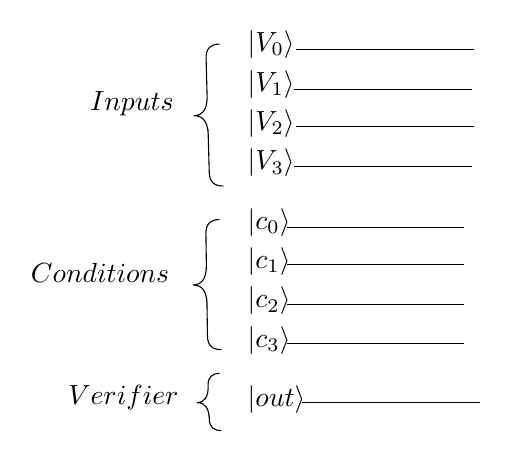
\begin{tikzpicture}[x=0.75pt,y=0.75pt,yscale=-0.95,xscale=0.95]
%uncomment if require: \path (0,300); %set diagram left start at 0, and has height of 300

%Shape: Brace [id:dp6153728275164612] 
\draw   (158,40) .. controls (153.33,40.13) and (151.07,42.52) .. (151.2,47.19) -- (151.72,66.2) .. controls (151.91,72.86) and (149.67,76.26) .. (145,76.39) .. controls (149.67,76.26) and (152.09,79.52) .. (152.28,86.19)(152.2,83.19) -- (152.81,105.2) .. controls (152.94,109.86) and (155.33,112.13) .. (160,112) ;
%Shape: Brace [id:dp8574558637937255] 
\draw   (158,129) .. controls (153.33,129.07) and (151.04,131.44) .. (151.11,136.11) -- (151.35,152.11) .. controls (151.45,158.78) and (149.17,162.14) .. (144.5,162.21) .. controls (149.17,162.14) and (151.55,165.44) .. (151.65,172.11)(151.61,169.11) -- (151.9,188.11) .. controls (151.97,192.78) and (154.33,195.07) .. (159,195) ;
%Shape: Brace [id:dp4003911472766615] 
\draw   (158,207) .. controls (154.02,207.14) and (152.1,209.2) .. (152.23,213.18) -- (152.23,213.18) .. controls (152.43,218.87) and (150.54,221.78) .. (146.56,221.91) .. controls (150.54,221.78) and (152.63,224.55) .. (152.82,230.23)(152.73,227.68) -- (152.82,230.23) .. controls (152.96,234.22) and (155.02,236.14) .. (159,236) ;
%Straight Lines [id:da5442487593963699] 
\draw    (197,43) -- (287,43) ;
%Straight Lines [id:da29037512454573644] 
\draw    (196,63) -- (286,63) ;
%Straight Lines [id:da5479082959884316] 
\draw    (197,82) -- (287,82) ;
%Straight Lines [id:da11508947791683277] 
\draw    (192,172) -- (282,172) ;
%Straight Lines [id:da42718074868005385] 
\draw    (192,133) -- (282,133) ;
%Straight Lines [id:da8551579185541867] 
\draw    (192,192) -- (282,192) ;
%Straight Lines [id:da45397889708542727] 
\draw    (192,152) -- (282,152) ;
%Straight Lines [id:da5910100696477991] 
\draw    (200,222) -- (290,222) ;
%Straight Lines [id:da03425997175901285] 
\draw    (196,102) -- (286,102) ;

% Text Node
\draw (171,32) node [anchor=north west][inner sep=0.75pt]   [align=left] {$\displaystyle \ket{V_{0}}$};
% Text Node
\draw (171,122) node [anchor=north west][inner sep=0.75pt]   [align=left] {$\displaystyle \ket{c_{0}}$};
% Text Node
\draw (171,72) node [anchor=north west][inner sep=0.75pt]   [align=left] {$\displaystyle \ket{V_{2}}$};
% Text Node
\draw (171,52) node [anchor=north west][inner sep=0.75pt]   [align=left] {$\displaystyle \ket{V_{1}}$};
% Text Node
\draw (171,92) node [anchor=north west][inner sep=0.75pt]   [align=left] {$\displaystyle \ket{V_{3}}$};
% Text Node
\draw (171,142) node [anchor=north west][inner sep=0.75pt]   [align=left] {$\displaystyle \ket{c_{1}}$};
% Text Node
\draw (171,162) node [anchor=north west][inner sep=0.75pt]   [align=left] {$\displaystyle \ket{c_{2}}$};
% Text Node
\draw (171,182) node [anchor=north west][inner sep=0.75pt]   [align=left] {$\displaystyle \ket{c_{3}}$};
% Text Node
\draw (171,212) node [anchor=north west][inner sep=0.75pt]   [align=left] {$\displaystyle \ket{out}$};
% Text Node
\draw (91,63) node [anchor=north west][inner sep=0.75pt]   [align=left] {$\displaystyle Inputs$};
% Text Node
\draw (61,150) node [anchor=north west][inner sep=0.75pt]   [align=left] {$\displaystyle Conditions$};
% Text Node
\draw (80,212) node [anchor=north west][inner sep=0.75pt]   [align=left] {$\displaystyle Verifier$};


\end{tikzpicture}


    \caption{Sudoku Circuit Diagram 1}
    \label{fig:my_label}
\end{figure}

To be able to do this, this circuit is going to need a total of 9 qubits. The first 4 ($\ket{V\textsubscript{X}}$) will represent one of each element on the \textit{2x2} Sudoku board, the next 4 ($\ket{c}$) will represent one of the 4 rules for the board and the last qubit ($\ket{out}$) will act like a verifier which will tell us if the rules have been satisfied.
\pagebreak

\subsubsection{Defining the Sudoku Rules} \label{sudoku rules}

%picture{https://drive.google.com/file/d/1TeY8IskmDYT1ZgUDRdDvOoTcLCOyZQQM/view}

As mentioned in \ref{Making the Oracle 2x2}, the first thing we need to do is establish and define the rules for the inputs such that no adjacent numbers on the board are equal to each other. This means that:
\begin{enumerate}
    \item $V\textsubscript{0} \neq V\textsubscript{1}$
    \item $V\textsubscript{0} \neq V\textsubscript{2}$
    \item $V\textsubscript{1} \neq V\textsubscript{3}$ and, 
    \item $V\textsubscript{2} \neq V\textsubscript{3}$
\end{enumerate}

This is implemented as follows:

\begin{file}[def sudoku\_conditions(self) -> Matrix:]
\begin{lstlisting}[language=Python]
cond1 = g.control_x(9, [1], 4) * 
            g.control_x(9, [0], 4)
cond2 = g.control_x(9, [2], 5) * 
            g.control_x(9, [0], 5)
cond3 = g.control_x(9, [3], 6) * 
            g.control_x(9, [1], 6)
cond4 = g.control_x(9, [3], 7) * 
            g.control_x(9, [2], 7)

cond = cond4 * cond3 * cond2 * cond1

return cond
\end{lstlisting}
\end{file}

The rules listed 1-4 can be thought of as classical XOR gates acting on the qubits which represent $\ket{V\textsubscript{X}}$ and the result is stored in the condition qubits $\ket{c}$. Looking at the variable \textit{cond1}, we create an XOR gate by applying two Control-X gates, one with the 0th qubit as the control, the other with the 1st qubit as the control; both results are stored into the 4th qubit, the $c\textsubscript{1}$ qubit. 
We do this for each condition/rule and multiply all the gates together to get one big matrix which will be returned by this function.
\begin{figure}[h]
    \centering
    
\begin{center}
\tikzset{every picture/.style={line width=0.75pt}} %set default line width to 0.75pt        

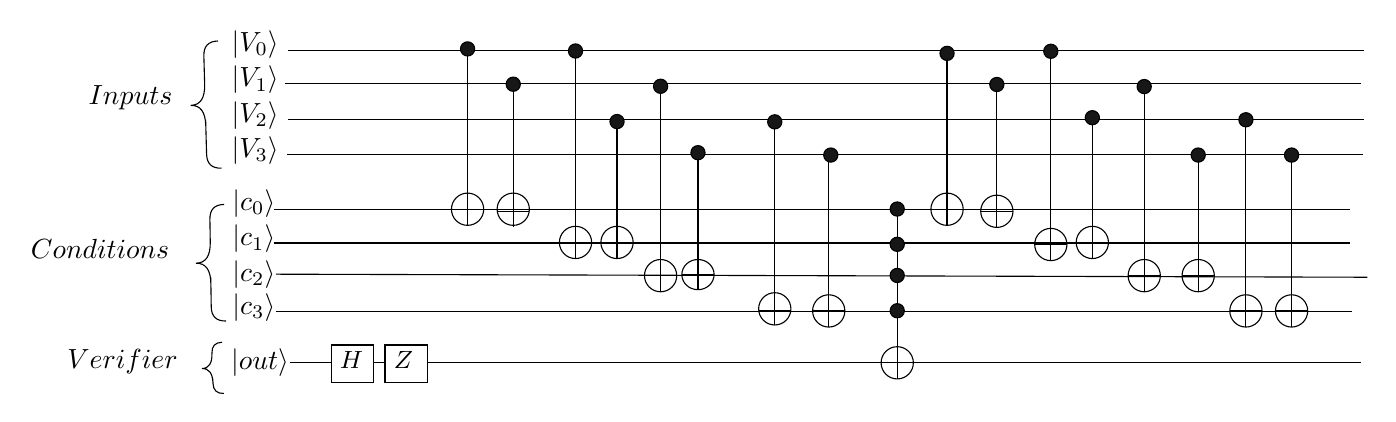
\begin{tikzpicture}[x=0.75pt,y=0.75pt,yscale=-1,xscale=1]
%uncomment if require: \path (0,300); %set diagram left start at 0, and has height of 300

%Shape: Brace [id:dp20561472354056276] 
\draw   (94.51,58.51) .. controls (89.85,58.64) and (87.58,61.04) .. (87.71,65.7) -- (88.09,79.35) .. controls (88.28,86.02) and (86.04,89.41) .. (81.37,89.54) .. controls (86.04,89.41) and (88.46,92.68) .. (88.64,99.34)(88.56,96.34) -- (89.02,112.99) .. controls (89.15,117.65) and (91.55,119.92) .. (96.21,119.79) ;
%Shape: Brace [id:dp7742338662074237] 
\draw   (97.51,137.26) .. controls (92.84,137.33) and (90.55,139.7) .. (90.62,144.36) -- (90.79,155.45) .. controls (90.89,162.12) and (88.61,165.49) .. (83.94,165.56) .. controls (88.61,165.49) and (90.99,168.78) .. (91.09,175.45)(91.05,172.45) -- (91.26,186.54) .. controls (91.33,191.21) and (93.7,193.5) .. (98.37,193.43) ;
%Shape: Brace [id:dp7717937487234783] 
\draw   (96.51,203.65) .. controls (93.12,203.76) and (91.49,205.51) .. (91.61,208.9) -- (91.61,208.9) .. controls (91.78,213.74) and (90.17,216.22) .. (86.78,216.34) .. controls (90.17,216.22) and (91.94,218.58) .. (92.11,223.42)(92.03,221.24) -- (92.11,223.42) .. controls (92.22,226.81) and (93.98,228.44) .. (97.37,228.33) ;
%Straight Lines [id:da7300954727834195] 
\draw    (128.13,63.06) -- (646.51,63.06) ;
%Straight Lines [id:da4408679081521467] 
\draw    (126.76,79.09) -- (645.15,79.09) ;
%Straight Lines [id:da655005386836327] 
\draw    (128.13,96.26) -- (646.51,96.26) ;
%Straight Lines [id:da09915301858685255] 
\draw    (122.41,170.86) -- (648.24,172.33) ;
%Straight Lines [id:da013610689769587792] 
\draw    (121.31,139.66) -- (639.69,139.66) ;
%Straight Lines [id:da6172496695616365] 
\draw    (122.41,188.88) -- (640.79,188.88) ;
%Straight Lines [id:da4038233729649441] 
\draw    (121.31,155.83) -- (639.69,155.83) ;
%Straight Lines [id:da6326322967955269] 
\draw    (129.31,213.41) -- (645.22,213.41) ;
%Straight Lines [id:da7686626921998831] 
\draw    (127.86,113.28) -- (646.25,113.28) ;
%Shape: Circle [id:dp7441809312999461] 
\draw   (207,139.56) .. controls (207,135.27) and (210.48,131.79) .. (214.77,131.79) .. controls (219.06,131.79) and (222.54,135.27) .. (222.54,139.56) .. controls (222.54,143.85) and (219.06,147.33) .. (214.77,147.33) .. controls (210.48,147.33) and (207,143.85) .. (207,139.56) -- cycle ;
%Straight Lines [id:da8659846293923357] 
\draw    (207,139.56) -- (222.54,139.56) ;
%Straight Lines [id:da024312662446195343] 
\draw    (214.77,62.33) -- (214.77,147.33) ;
%Shape: Circle [id:dp4630459231419892] 
\draw   (229,139.56) .. controls (229,135.27) and (232.48,131.79) .. (236.77,131.79) .. controls (241.06,131.79) and (244.54,135.27) .. (244.54,139.56) .. controls (244.54,143.85) and (241.06,147.33) .. (236.77,147.33) .. controls (232.48,147.33) and (229,143.85) .. (229,139.56) -- cycle ;
%Straight Lines [id:da8360715536385481] 
\draw    (229,140.56) -- (244.54,140.56) ;
%Straight Lines [id:da1511835484730215] 
\draw    (236.77,78.33) -- (236.77,148.33) ;
%Shape: Circle [id:dp5288352035682198] 
\draw   (259,155.56) .. controls (259,151.27) and (262.48,147.79) .. (266.77,147.79) .. controls (271.06,147.79) and (274.54,151.27) .. (274.54,155.56) .. controls (274.54,159.85) and (271.06,163.33) .. (266.77,163.33) .. controls (262.48,163.33) and (259,159.85) .. (259,155.56) -- cycle ;
%Straight Lines [id:da7528094688377307] 
\draw    (259,155.56) -- (274.54,155.56) ;
%Straight Lines [id:da9361429999090938] 
\draw    (266.77,63.33) -- (266.77,163.33) ;
%Shape: Circle [id:dp33491036565000765] 
\draw   (279,155.56) .. controls (279,151.27) and (282.48,147.79) .. (286.77,147.79) .. controls (291.06,147.79) and (294.54,151.27) .. (294.54,155.56) .. controls (294.54,159.85) and (291.06,163.33) .. (286.77,163.33) .. controls (282.48,163.33) and (279,159.85) .. (279,155.56) -- cycle ;
%Straight Lines [id:da26144271190549384] 
\draw    (279,155.56) -- (294.54,155.56) ;
%Straight Lines [id:da5874562865115387] 
\draw    (286.77,97.33) -- (286.77,163.33) ;
%Shape: Circle [id:dp5636247166959916] 
\draw   (300,171.56) .. controls (300,167.27) and (303.48,163.79) .. (307.77,163.79) .. controls (312.06,163.79) and (315.54,167.27) .. (315.54,171.56) .. controls (315.54,175.85) and (312.06,179.33) .. (307.77,179.33) .. controls (303.48,179.33) and (300,175.85) .. (300,171.56) -- cycle ;
%Straight Lines [id:da021789390921582497] 
\draw    (300,171.56) -- (315.54,171.56) ;
%Straight Lines [id:da24634333457351998] 
\draw    (307.77,78.47) -- (307.77,179.33) ;
%Shape: Ellipse [id:dp9824533507386775] 
\draw   (318,171.06) .. controls (318,167.04) and (321.48,163.79) .. (325.77,163.79) .. controls (330.06,163.79) and (333.54,167.04) .. (333.54,171.06) .. controls (333.54,175.08) and (330.06,178.33) .. (325.77,178.33) .. controls (321.48,178.33) and (318,175.08) .. (318,171.06) -- cycle ;
%Straight Lines [id:da825910541988566] 
\draw    (318,171.06) -- (333.54,171.06) ;
%Straight Lines [id:da1107058770647007] 
\draw    (325.77,112.33) -- (325.77,178.33) ;
%Shape: Circle [id:dp09596694759481861] 
\draw   (355,187.56) .. controls (355,183.27) and (358.48,179.79) .. (362.77,179.79) .. controls (367.06,179.79) and (370.54,183.27) .. (370.54,187.56) .. controls (370.54,191.85) and (367.06,195.33) .. (362.77,195.33) .. controls (358.48,195.33) and (355,191.85) .. (355,187.56) -- cycle ;
%Straight Lines [id:da5539250315761879] 
\draw    (355,188.56) -- (370.54,188.56) ;
%Straight Lines [id:da7319963193642351] 
\draw    (362.77,97.47) -- (362.77,195.33) ;
%Shape: Circle [id:dp661519371279361] 
\draw   (381,188.56) .. controls (381,184.27) and (384.48,180.79) .. (388.77,180.79) .. controls (393.06,180.79) and (396.54,184.27) .. (396.54,188.56) .. controls (396.54,192.85) and (393.06,196.33) .. (388.77,196.33) .. controls (384.48,196.33) and (381,192.85) .. (381,188.56) -- cycle ;
%Straight Lines [id:da05304329978786759] 
\draw    (381,188.56) -- (396.54,188.56) ;
%Straight Lines [id:da4444917240308277] 
\draw    (388.77,113.47) -- (388.77,196.33) ;
%Shape: Circle [id:dp7689393862968612] 
\draw   (414,213.56) .. controls (414,209.27) and (417.48,205.79) .. (421.77,205.79) .. controls (426.06,205.79) and (429.54,209.27) .. (429.54,213.56) .. controls (429.54,217.85) and (426.06,221.33) .. (421.77,221.33) .. controls (417.48,221.33) and (414,217.85) .. (414,213.56) -- cycle ;
%Straight Lines [id:da059336099485750804] 
\draw    (414,213.56) -- (429.54,213.56) ;
%Straight Lines [id:da36789924920470063] 
\draw    (421.77,138.47) -- (421.77,221.33) ;
%Shape: Circle [id:dp1693172014573172] 
\draw   (438,139.56) .. controls (438,135.27) and (441.48,131.79) .. (445.77,131.79) .. controls (450.06,131.79) and (453.54,135.27) .. (453.54,139.56) .. controls (453.54,143.85) and (450.06,147.33) .. (445.77,147.33) .. controls (441.48,147.33) and (438,143.85) .. (438,139.56) -- cycle ;
%Straight Lines [id:da572098582586902] 
\draw    (438,139.56) -- (453.54,139.56) ;
%Straight Lines [id:da9348802969204693] 
\draw    (445.77,63.47) -- (445.77,147.33) ;
%Shape: Circle [id:dp3374297233505197] 
\draw   (462,140.56) .. controls (462,136.27) and (465.48,132.79) .. (469.77,132.79) .. controls (474.06,132.79) and (477.54,136.27) .. (477.54,140.56) .. controls (477.54,144.85) and (474.06,148.33) .. (469.77,148.33) .. controls (465.48,148.33) and (462,144.85) .. (462,140.56) -- cycle ;
%Straight Lines [id:da3978023214414772] 
\draw    (462,140.56) -- (477.54,140.56) ;
%Straight Lines [id:da5137215515262947] 
\draw    (469.77,79.47) -- (469.77,148.33) ;
%Shape: Circle [id:dp28925146103868915] 
\draw   (488,156.56) .. controls (488,152.27) and (491.48,148.79) .. (495.77,148.79) .. controls (500.06,148.79) and (503.54,152.27) .. (503.54,156.56) .. controls (503.54,160.85) and (500.06,164.33) .. (495.77,164.33) .. controls (491.48,164.33) and (488,160.85) .. (488,156.56) -- cycle ;
%Straight Lines [id:da32484367017285765] 
\draw    (488,156.56) -- (503.54,156.56) ;
%Straight Lines [id:da4011889098051864] 
\draw    (495.77,64.47) -- (495.77,164.33) ;
%Shape: Circle [id:dp2836997083710966] 
\draw   (508,155.56) .. controls (508,151.27) and (511.48,147.79) .. (515.77,147.79) .. controls (520.06,147.79) and (523.54,151.27) .. (523.54,155.56) .. controls (523.54,159.85) and (520.06,163.33) .. (515.77,163.33) .. controls (511.48,163.33) and (508,159.85) .. (508,155.56) -- cycle ;
%Straight Lines [id:da4474028608676359] 
\draw    (508,155.56) -- (523.54,155.56) ;
%Straight Lines [id:da21990490071010638] 
\draw    (515.77,96.47) -- (515.77,163.33) ;
%Shape: Circle [id:dp6977615807686228] 
\draw   (533,171.56) .. controls (533,167.27) and (536.48,163.79) .. (540.77,163.79) .. controls (545.06,163.79) and (548.54,167.27) .. (548.54,171.56) .. controls (548.54,175.85) and (545.06,179.33) .. (540.77,179.33) .. controls (536.48,179.33) and (533,175.85) .. (533,171.56) -- cycle ;
%Straight Lines [id:da40329106353901456] 
\draw    (533,171.56) -- (548.54,171.56) ;
%Straight Lines [id:da5323975523166089] 
\draw    (540.77,79.47) -- (540.77,179.33) ;
%Shape: Circle [id:dp5909908367646703] 
\draw   (559,171.56) .. controls (559,167.27) and (562.48,163.79) .. (566.77,163.79) .. controls (571.06,163.79) and (574.54,167.27) .. (574.54,171.56) .. controls (574.54,175.85) and (571.06,179.33) .. (566.77,179.33) .. controls (562.48,179.33) and (559,175.85) .. (559,171.56) -- cycle ;
%Straight Lines [id:da8587141386565724] 
\draw    (559,171.56) -- (574.54,171.56) ;
%Straight Lines [id:da9917642704603606] 
\draw    (566.77,113.47) -- (566.77,179.33) ;
%Shape: Circle [id:dp8381277920907859] 
\draw   (582,188.56) .. controls (582,184.27) and (585.48,180.79) .. (589.77,180.79) .. controls (594.06,180.79) and (597.54,184.27) .. (597.54,188.56) .. controls (597.54,192.85) and (594.06,196.33) .. (589.77,196.33) .. controls (585.48,196.33) and (582,192.85) .. (582,188.56) -- cycle ;
%Straight Lines [id:da03031862305325661] 
\draw    (582,188.56) -- (597.54,188.56) ;
%Straight Lines [id:da0702663365262608] 
\draw    (589.77,96.47) -- (589.77,196.33) ;
%Shape: Circle [id:dp24914976725722182] 
\draw   (604,188.56) .. controls (604,184.27) and (607.48,180.79) .. (611.77,180.79) .. controls (616.06,180.79) and (619.54,184.27) .. (619.54,188.56) .. controls (619.54,192.85) and (616.06,196.33) .. (611.77,196.33) .. controls (607.48,196.33) and (604,192.85) .. (604,188.56) -- cycle ;
%Straight Lines [id:da5779211452274127] 
\draw    (604,188.56) -- (619.54,188.56) ;
%Straight Lines [id:da9193786715165126] 
\draw    (611.77,114.47) -- (611.77,196.33) ;
%Shape: Circle [id:dp6304720191778563] 
\draw  [fill={rgb, 255:red, 23; green, 23; blue, 23 }  ,fill opacity=1 ] (218.19,62.33) .. controls (218.19,60.44) and (216.66,58.91) .. (214.77,58.91) .. controls (212.88,58.91) and (211.35,60.44) .. (211.35,62.33) .. controls (211.35,64.22) and (212.88,65.75) .. (214.77,65.75) .. controls (216.66,65.75) and (218.19,64.22) .. (218.19,62.33) -- cycle ;
%Shape: Circle [id:dp8929190250098362] 
\draw  [fill={rgb, 255:red, 23; green, 23; blue, 23 }  ,fill opacity=1 ] (240.19,79.33) .. controls (240.19,77.44) and (238.66,75.91) .. (236.77,75.91) .. controls (234.88,75.91) and (233.35,77.44) .. (233.35,79.33) .. controls (233.35,81.22) and (234.88,82.75) .. (236.77,82.75) .. controls (238.66,82.75) and (240.19,81.22) .. (240.19,79.33) -- cycle ;
%Shape: Circle [id:dp2920270195756338] 
\draw  [fill={rgb, 255:red, 23; green, 23; blue, 23 }  ,fill opacity=1 ] (270.19,63.33) .. controls (270.19,61.44) and (268.66,59.91) .. (266.77,59.91) .. controls (264.88,59.91) and (263.35,61.44) .. (263.35,63.33) .. controls (263.35,65.22) and (264.88,66.75) .. (266.77,66.75) .. controls (268.66,66.75) and (270.19,65.22) .. (270.19,63.33) -- cycle ;
%Shape: Circle [id:dp6499562942127359] 
\draw  [fill={rgb, 255:red, 23; green, 23; blue, 23 }  ,fill opacity=1 ] (290.19,97.33) .. controls (290.19,95.44) and (288.66,93.91) .. (286.77,93.91) .. controls (284.88,93.91) and (283.35,95.44) .. (283.35,97.33) .. controls (283.35,99.22) and (284.88,100.75) .. (286.77,100.75) .. controls (288.66,100.75) and (290.19,99.22) .. (290.19,97.33) -- cycle ;
%Shape: Circle [id:dp6406575637511018] 
\draw  [fill={rgb, 255:red, 23; green, 23; blue, 23 }  ,fill opacity=1 ] (311.19,80.33) .. controls (311.19,78.44) and (309.66,76.91) .. (307.77,76.91) .. controls (305.88,76.91) and (304.35,78.44) .. (304.35,80.33) .. controls (304.35,82.22) and (305.88,83.75) .. (307.77,83.75) .. controls (309.66,83.75) and (311.19,82.22) .. (311.19,80.33) -- cycle ;
%Shape: Circle [id:dp7285996494543623] 
\draw  [fill={rgb, 255:red, 23; green, 23; blue, 23 }  ,fill opacity=1 ] (329.19,112.33) .. controls (329.19,110.44) and (327.66,108.91) .. (325.77,108.91) .. controls (323.88,108.91) and (322.35,110.44) .. (322.35,112.33) .. controls (322.35,114.22) and (323.88,115.75) .. (325.77,115.75) .. controls (327.66,115.75) and (329.19,114.22) .. (329.19,112.33) -- cycle ;
%Shape: Circle [id:dp5821939599103578] 
\draw  [fill={rgb, 255:red, 23; green, 23; blue, 23 }  ,fill opacity=1 ] (366.19,97.47) .. controls (366.19,95.58) and (364.66,94.05) .. (362.77,94.05) .. controls (360.88,94.05) and (359.35,95.58) .. (359.35,97.47) .. controls (359.35,99.36) and (360.88,100.89) .. (362.77,100.89) .. controls (364.66,100.89) and (366.19,99.36) .. (366.19,97.47) -- cycle ;
%Shape: Circle [id:dp013073544677321136] 
\draw  [fill={rgb, 255:red, 23; green, 23; blue, 23 }  ,fill opacity=1 ] (393.19,113.47) .. controls (393.19,111.58) and (391.66,110.05) .. (389.77,110.05) .. controls (387.88,110.05) and (386.35,111.58) .. (386.35,113.47) .. controls (386.35,115.36) and (387.88,116.89) .. (389.77,116.89) .. controls (391.66,116.89) and (393.19,115.36) .. (393.19,113.47) -- cycle ;
%Shape: Circle [id:dp5856658676000039] 
\draw  [fill={rgb, 255:red, 23; green, 23; blue, 23 }  ,fill opacity=1 ] (425.19,139.47) .. controls (425.19,137.58) and (423.66,136.05) .. (421.77,136.05) .. controls (419.88,136.05) and (418.35,137.58) .. (418.35,139.47) .. controls (418.35,141.36) and (419.88,142.89) .. (421.77,142.89) .. controls (423.66,142.89) and (425.19,141.36) .. (425.19,139.47) -- cycle ;
%Shape: Circle [id:dp8599888390696802] 
\draw  [fill={rgb, 255:red, 23; green, 23; blue, 23 }  ,fill opacity=1 ] (425.19,156.47) .. controls (425.19,154.58) and (423.66,153.05) .. (421.77,153.05) .. controls (419.88,153.05) and (418.35,154.58) .. (418.35,156.47) .. controls (418.35,158.36) and (419.88,159.89) .. (421.77,159.89) .. controls (423.66,159.89) and (425.19,158.36) .. (425.19,156.47) -- cycle ;
%Shape: Circle [id:dp5662559531507205] 
\draw  [fill={rgb, 255:red, 23; green, 23; blue, 23 }  ,fill opacity=1 ] (425.19,171.47) .. controls (425.19,169.58) and (423.66,168.05) .. (421.77,168.05) .. controls (419.88,168.05) and (418.35,169.58) .. (418.35,171.47) .. controls (418.35,173.36) and (419.88,174.89) .. (421.77,174.89) .. controls (423.66,174.89) and (425.19,173.36) .. (425.19,171.47) -- cycle ;
%Shape: Circle [id:dp4978649289043018] 
\draw  [fill={rgb, 255:red, 23; green, 23; blue, 23 }  ,fill opacity=1 ] (425.19,188.47) .. controls (425.19,186.58) and (423.66,185.05) .. (421.77,185.05) .. controls (419.88,185.05) and (418.35,186.58) .. (418.35,188.47) .. controls (418.35,190.36) and (419.88,191.89) .. (421.77,191.89) .. controls (423.66,191.89) and (425.19,190.36) .. (425.19,188.47) -- cycle ;
%Shape: Circle [id:dp31128731995412773] 
\draw  [fill={rgb, 255:red, 23; green, 23; blue, 23 }  ,fill opacity=1 ] (449.19,64.47) .. controls (449.19,62.58) and (447.66,61.05) .. (445.77,61.05) .. controls (443.88,61.05) and (442.35,62.58) .. (442.35,64.47) .. controls (442.35,66.36) and (443.88,67.89) .. (445.77,67.89) .. controls (447.66,67.89) and (449.19,66.36) .. (449.19,64.47) -- cycle ;
%Shape: Circle [id:dp7356858476825425] 
\draw  [fill={rgb, 255:red, 23; green, 23; blue, 23 }  ,fill opacity=1 ] (473.19,79.47) .. controls (473.19,77.58) and (471.66,76.05) .. (469.77,76.05) .. controls (467.88,76.05) and (466.35,77.58) .. (466.35,79.47) .. controls (466.35,81.36) and (467.88,82.89) .. (469.77,82.89) .. controls (471.66,82.89) and (473.19,81.36) .. (473.19,79.47) -- cycle ;
%Shape: Circle [id:dp16150718271163078] 
\draw  [fill={rgb, 255:red, 23; green, 23; blue, 23 }  ,fill opacity=1 ] (499.19,63.47) .. controls (499.19,61.58) and (497.66,60.05) .. (495.77,60.05) .. controls (493.88,60.05) and (492.35,61.58) .. (492.35,63.47) .. controls (492.35,65.36) and (493.88,66.89) .. (495.77,66.89) .. controls (497.66,66.89) and (499.19,65.36) .. (499.19,63.47) -- cycle ;
%Shape: Circle [id:dp18668823047568317] 
\draw  [fill={rgb, 255:red, 23; green, 23; blue, 23 }  ,fill opacity=1 ] (519.19,95.47) .. controls (519.19,93.58) and (517.66,92.05) .. (515.77,92.05) .. controls (513.88,92.05) and (512.35,93.58) .. (512.35,95.47) .. controls (512.35,97.36) and (513.88,98.89) .. (515.77,98.89) .. controls (517.66,98.89) and (519.19,97.36) .. (519.19,95.47) -- cycle ;
%Shape: Circle [id:dp2960756940650524] 
\draw  [fill={rgb, 255:red, 23; green, 23; blue, 23 }  ,fill opacity=1 ] (544.19,80.47) .. controls (544.19,78.58) and (542.66,77.05) .. (540.77,77.05) .. controls (538.88,77.05) and (537.35,78.58) .. (537.35,80.47) .. controls (537.35,82.36) and (538.88,83.89) .. (540.77,83.89) .. controls (542.66,83.89) and (544.19,82.36) .. (544.19,80.47) -- cycle ;
%Shape: Circle [id:dp7654405098838482] 
\draw  [fill={rgb, 255:red, 23; green, 23; blue, 23 }  ,fill opacity=1 ] (570.19,113.47) .. controls (570.19,111.58) and (568.66,110.05) .. (566.77,110.05) .. controls (564.88,110.05) and (563.35,111.58) .. (563.35,113.47) .. controls (563.35,115.36) and (564.88,116.89) .. (566.77,116.89) .. controls (568.66,116.89) and (570.19,115.36) .. (570.19,113.47) -- cycle ;
%Shape: Circle [id:dp3878512491995376] 
\draw  [fill={rgb, 255:red, 23; green, 23; blue, 23 }  ,fill opacity=1 ] (593.19,96.47) .. controls (593.19,94.58) and (591.66,93.05) .. (589.77,93.05) .. controls (587.88,93.05) and (586.35,94.58) .. (586.35,96.47) .. controls (586.35,98.36) and (587.88,99.89) .. (589.77,99.89) .. controls (591.66,99.89) and (593.19,98.36) .. (593.19,96.47) -- cycle ;
%Shape: Circle [id:dp98039518274487] 
\draw  [fill={rgb, 255:red, 23; green, 23; blue, 23 }  ,fill opacity=1 ] (615.19,113.47) .. controls (615.19,111.58) and (613.66,110.05) .. (611.77,110.05) .. controls (609.88,110.05) and (608.35,111.58) .. (608.35,113.47) .. controls (608.35,115.36) and (609.88,116.89) .. (611.77,116.89) .. controls (613.66,116.89) and (615.19,115.36) .. (615.19,113.47) -- cycle ;
%Shape: Rectangle [id:dp29591413416439916] 
\draw  [fill={rgb, 255:red, 255; green, 255; blue, 255 }  ,fill opacity=1 ] (149,205) -- (169.52,205) -- (169.52,223.13) -- (149,223.13) -- cycle ;

%Shape: Rectangle [id:dp5477743831103108] 
\draw  [fill={rgb, 255:red, 255; green, 255; blue, 255 }  ,fill opacity=1 ] (175,205) -- (195.52,205) -- (195.52,223.13) -- (175,223.13) -- cycle ;


% Text Node
\draw (99.86,52.36) node [anchor=north west][inner sep=0.75pt]   [align=left] {$\displaystyle \ket{V_{0}}$};
% Text Node
\draw (100.23,128.96) node [anchor=north west][inner sep=0.75pt]   [align=left] {$\displaystyle \ket{c_{0}}$};
% Text Node
\draw (99.86,86.41) node [anchor=north west][inner sep=0.75pt]   [align=left] {$\displaystyle \ket{V_{2}}$};
% Text Node
\draw (99.86,69.38) node [anchor=north west][inner sep=0.75pt]   [align=left] {$\displaystyle \ket{V_{1}}$};
% Text Node
\draw (99.86,103.43) node [anchor=north west][inner sep=0.75pt]   [align=left] {$\displaystyle \ket{V_{3}}$};
% Text Node
\draw (100.23,145.98) node [anchor=north west][inner sep=0.75pt]   [align=left] {$\displaystyle \ket{c_{1}}$};
% Text Node
\draw (100.23,163.01) node [anchor=north west][inner sep=0.75pt]   [align=left] {$\displaystyle \ket{c_{2}}$};
% Text Node
\draw (100.23,179.03) node [anchor=north west][inner sep=0.75pt]   [align=left] {$\displaystyle \ket{c_{3}}$};
% Text Node
\draw (99.63,205.56) node [anchor=north west][inner sep=0.75pt]   [align=left] {$\displaystyle \ket{out}$};
% Text Node
\draw (30.94,78.75) node [anchor=north west][inner sep=0.75pt]   [align=left] {$\displaystyle Inputs$};
% Text Node
\draw (3.09,152.79) node [anchor=north west][inner sep=0.75pt]   [align=left] {$\displaystyle Conditions$};
% Text Node
\draw (20.68,205.56) node [anchor=north west][inner sep=0.75pt]   [align=left] {$\displaystyle Verifier$};
% Text Node
\draw (152,207) node [anchor=north west][inner sep=0.75pt]  [font=\small] [align=left] {$\displaystyle H$};
% Text Node
\draw (178,207) node [anchor=north west][inner sep=0.75pt]  [font=\small] [align=left] {$\displaystyle Z$};


\end{tikzpicture}
\end{center}
    \caption{Sudoku Circuit Diagram 2}
    \label{fig:my_label}
\end{figure}
\pagebreak

\subsubsection{Oracle}
\begin{file}[def oracle(self) -> Matrix:]
\centering
\begin{lstlisting}[language=Python]
had = g.multi_gate(9, [8], g.Gate.H)
z = g.multi_gate(9, [8], g.Gate.Z)
cond = self.sudoku_conditions()
cnot = g.control_x(9, [4, 5, 6, 7], 8)
oracle = cond * cnot * cond
oracle = cond * cnot * cond * z * had
return oracle
\end{lstlisting}
\end{file}

Now that the rules for the sudoku board have been established we now need to implement the oracle gate. This is done in a few short steps:
\begin{itemize}
    \item Firstly, we apply a Hadamard followed by a phase shift gate to the Output qubit $\ket{out}$ to get the state $\ket{-} = \ket{0} - \ket{1}$.
    \item Next, we determine whether all of the conditions have been met by applying a Control-X gate, where all the condition qubits $\ket{c}$ are the controls and the Output qubit $\ket{out}$ is the target.
    \item Lastly, we reset all the values in the condition qubits such that we can use the Oracle again later without having propagating errors and then return the resulting matrix
\end{itemize}
\begin{figure}[h]
    \centering
    


\tikzset{every picture/.style={line width=0.75pt}} %set default line width to 0.75pt        

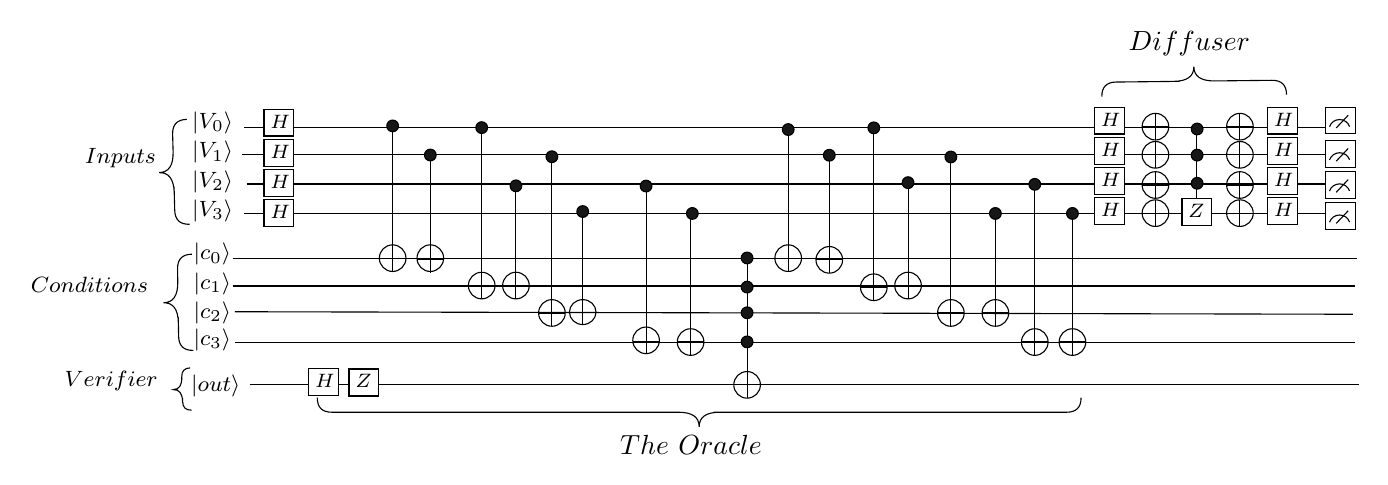
\begin{tikzpicture}[x=0.75pt,y=0.75pt,yscale=-1,xscale=1]
%uncomment if require: \path (0,300); %set diagram left start at 0, and has height of 300

%Shape: Brace [id:dp013847914349599089] 
\draw   (82.42,59.91) .. controls (77.76,60.04) and (75.49,62.43) .. (75.62,67.1) -- (75.85,75.38) .. controls (76.04,82.05) and (73.8,85.44) .. (69.13,85.57) .. controls (73.8,85.44) and (76.22,88.71) .. (76.4,95.38)(76.32,92.38) -- (76.63,103.66) .. controls (76.76,108.33) and (79.16,110.59) .. (83.83,110.46) ;
%Shape: Brace [id:dp06222432164001401] 
\draw   (84.9,124.87) .. controls (80.23,124.94) and (77.93,127.31) .. (78,131.98) -- (78.1,138.15) .. controls (78.2,144.82) and (75.92,148.19) .. (71.25,148.26) .. controls (75.92,148.19) and (78.3,151.48) .. (78.4,158.15)(78.36,155.15) -- (78.5,164.32) .. controls (78.57,168.99) and (80.93,171.29) .. (85.6,171.22) ;
%Shape: Brace [id:dp9402091488444337] 
\draw   (84.07,179.64) .. controls (81.28,179.74) and (79.93,181.19) .. (80.03,183.98) -- (80.03,183.98) .. controls (80.16,187.97) and (78.83,190.02) .. (76.04,190.11) .. controls (78.83,190.02) and (80.3,191.97) .. (80.44,195.96)(80.38,194.16) -- (80.44,195.96) .. controls (80.53,198.75) and (81.98,200.1) .. (84.78,200) ;
%Straight Lines [id:da7646287963192218] 
\draw    (110.22,63.67) -- (638.31,63.67) ;
%Straight Lines [id:da9764362326688856] 
\draw    (109.03,76.88) -- (635.23,76.88) ;
%Straight Lines [id:da6602273673301782] 
\draw    (111.23,91.05) -- (636.23,91.05) ;
%Straight Lines [id:da6151916745839932] 
\draw    (105.65,152.59) -- (644.28,153.81) ;
%Straight Lines [id:da7820434553041149] 
\draw    (104.53,126.86) -- (646.3,126.86) ;
%Straight Lines [id:da11624625723327409] 
\draw    (105.65,167.46) -- (645.31,167.46) ;
%Straight Lines [id:da28380413229506485] 
\draw    (104.53,140.2) -- (645.29,140.2) ;
%Straight Lines [id:da8936562173253038] 
\draw    (112.72,187.7) -- (647.31,187.7) ;
%Straight Lines [id:da5721556237428456] 
\draw    (109.99,105.09) -- (635.23,105.09) ;
%Shape: Ellipse [id:dp3486280662507839] 
\draw   (175.22,126.78) .. controls (175.22,123.24) and (178.09,120.37) .. (181.63,120.37) .. controls (185.17,120.37) and (188.04,123.24) .. (188.04,126.78) .. controls (188.04,130.32) and (185.17,133.19) .. (181.63,133.19) .. controls (178.09,133.19) and (175.22,130.32) .. (175.22,126.78) -- cycle ;
%Straight Lines [id:da8128272422226077] 
\draw    (175.22,126.78) -- (188.04,126.78) ;
%Straight Lines [id:da12449366923163918] 
\draw    (181.63,63.06) -- (181.63,133.19) ;
%Shape: Ellipse [id:dp656739879362918] 
\draw   (193.37,126.78) .. controls (193.37,123.24) and (196.24,120.37) .. (199.78,120.37) .. controls (203.32,120.37) and (206.19,123.24) .. (206.19,126.78) .. controls (206.19,130.32) and (203.32,133.19) .. (199.78,133.19) .. controls (196.24,133.19) and (193.37,130.32) .. (193.37,126.78) -- cycle ;
%Straight Lines [id:da02585359726941272] 
\draw    (193.37,127.6) -- (206.19,127.6) ;
%Straight Lines [id:da40356383190725875] 
\draw    (199.78,76.26) -- (199.78,134.01) ;
%Shape: Ellipse [id:dp14487484319959187] 
\draw   (218.12,139.98) .. controls (218.12,136.44) and (220.99,133.57) .. (224.53,133.57) .. controls (228.07,133.57) and (230.94,136.44) .. (230.94,139.98) .. controls (230.94,143.52) and (228.07,146.39) .. (224.53,146.39) .. controls (220.99,146.39) and (218.12,143.52) .. (218.12,139.98) -- cycle ;
%Straight Lines [id:da07026616653756856] 
\draw    (218.12,139.98) -- (230.94,139.98) ;
%Straight Lines [id:da5318804666225754] 
\draw    (224.53,63.89) -- (224.53,146.39) ;
%Shape: Ellipse [id:dp11098259954576473] 
\draw   (234.62,139.98) .. controls (234.62,136.44) and (237.49,133.57) .. (241.03,133.57) .. controls (244.57,133.57) and (247.44,136.44) .. (247.44,139.98) .. controls (247.44,143.52) and (244.57,146.39) .. (241.03,146.39) .. controls (237.49,146.39) and (234.62,143.52) .. (234.62,139.98) -- cycle ;
%Straight Lines [id:da16835734217823384] 
\draw    (234.62,139.98) -- (247.44,139.98) ;
%Straight Lines [id:da8548612509186462] 
\draw    (241.03,91.94) -- (241.03,146.39) ;
%Shape: Ellipse [id:dp8379415456483217] 
\draw   (251.95,153.18) .. controls (251.95,149.64) and (254.82,146.77) .. (258.36,146.77) .. controls (261.9,146.77) and (264.77,149.64) .. (264.77,153.18) .. controls (264.77,156.72) and (261.9,159.59) .. (258.36,159.59) .. controls (254.82,159.59) and (251.95,156.72) .. (251.95,153.18) -- cycle ;
%Straight Lines [id:da02996969780252523] 
\draw    (251.95,153.18) -- (264.77,153.18) ;
%Straight Lines [id:da023960571294774802] 
\draw    (258.36,76.37) -- (258.36,159.59) ;
%Shape: Ellipse [id:dp3250245241116676] 
\draw   (266.8,152.76) .. controls (266.8,149.45) and (269.67,146.76) .. (273.21,146.76) .. controls (276.75,146.76) and (279.61,149.45) .. (279.61,152.76) .. controls (279.61,156.07) and (276.75,158.76) .. (273.21,158.76) .. controls (269.67,158.76) and (266.8,156.07) .. (266.8,152.76) -- cycle ;
%Straight Lines [id:da7140531408850586] 
\draw    (266.8,152.76) -- (279.61,152.76) ;
%Straight Lines [id:da3904365925322162] 
\draw    (273.21,104.31) -- (273.21,158.76) ;
%Shape: Ellipse [id:dp3761518846524661] 
\draw   (297.32,166.38) .. controls (297.32,162.84) and (300.19,159.97) .. (303.73,159.97) .. controls (307.27,159.97) and (310.14,162.84) .. (310.14,166.38) .. controls (310.14,169.92) and (307.27,172.78) .. (303.73,172.78) .. controls (300.19,172.78) and (297.32,169.92) .. (297.32,166.38) -- cycle ;
%Straight Lines [id:da5973047741284501] 
\draw    (297.32,167.2) -- (310.14,167.2) ;
%Straight Lines [id:da2117892273602684] 
\draw    (303.73,92.05) -- (303.73,172.78) ;
%Shape: Ellipse [id:dp957820100674805] 
\draw   (318.77,167.2) .. controls (318.77,163.66) and (321.64,160.79) .. (325.18,160.79) .. controls (328.72,160.79) and (331.59,163.66) .. (331.59,167.2) .. controls (331.59,170.74) and (328.72,173.61) .. (325.18,173.61) .. controls (321.64,173.61) and (318.77,170.74) .. (318.77,167.2) -- cycle ;
%Straight Lines [id:da4425080652803781] 
\draw    (318.77,167.2) -- (331.59,167.2) ;
%Straight Lines [id:da1983801977236126] 
\draw    (325.18,105.25) -- (325.18,173.61) ;
%Shape: Ellipse [id:dp09725133860122126] 
\draw   (345.99,187.82) .. controls (345.99,184.28) and (348.86,181.41) .. (352.4,181.41) .. controls (355.94,181.41) and (358.81,184.28) .. (358.81,187.82) .. controls (358.81,191.36) and (355.94,194.23) .. (352.4,194.23) .. controls (348.86,194.23) and (345.99,191.36) .. (345.99,187.82) -- cycle ;
%Straight Lines [id:da6516124666604513] 
\draw    (345.99,187.82) -- (358.81,187.82) ;
%Straight Lines [id:da07085879710024123] 
\draw    (352.4,125.87) -- (352.4,194.23) ;
%Shape: Ellipse [id:dp9061011462576587] 
\draw   (365.79,126.78) .. controls (365.79,123.24) and (368.66,120.37) .. (372.2,120.37) .. controls (375.74,120.37) and (378.61,123.24) .. (378.61,126.78) .. controls (378.61,130.32) and (375.74,133.19) .. (372.2,133.19) .. controls (368.66,133.19) and (365.79,130.32) .. (365.79,126.78) -- cycle ;
%Straight Lines [id:da5218892620450915] 
\draw    (365.79,126.78) -- (378.61,126.78) ;
%Straight Lines [id:da8485179819781346] 
\draw    (372.2,64) -- (372.2,133.19) ;
%Shape: Ellipse [id:dp8937427664323856] 
\draw   (385.59,127.6) .. controls (385.59,124.06) and (388.46,121.19) .. (392,121.19) .. controls (395.54,121.19) and (398.41,124.06) .. (398.41,127.6) .. controls (398.41,131.14) and (395.54,134.01) .. (392,134.01) .. controls (388.46,134.01) and (385.59,131.14) .. (385.59,127.6) -- cycle ;
%Straight Lines [id:da5646398875251861] 
\draw    (385.59,127.6) -- (398.41,127.6) ;
%Straight Lines [id:da9894464654135591] 
\draw    (392,77.2) -- (392,134.01) ;
%Shape: Ellipse [id:dp3317065505160519] 
\draw   (407.04,140.8) .. controls (407.04,137.26) and (409.91,134.39) .. (413.45,134.39) .. controls (416.99,134.39) and (419.86,137.26) .. (419.86,140.8) .. controls (419.86,144.34) and (416.99,147.21) .. (413.45,147.21) .. controls (409.91,147.21) and (407.04,144.34) .. (407.04,140.8) -- cycle ;
%Straight Lines [id:da8305459605619017] 
\draw    (407.04,140.8) -- (419.86,140.8) ;
%Straight Lines [id:da4601376008936555] 
\draw    (413.45,64.82) -- (413.45,147.21) ;
%Shape: Ellipse [id:dp5530344456324341] 
\draw   (423.54,139.98) .. controls (423.54,136.44) and (426.41,133.57) .. (429.95,133.57) .. controls (433.49,133.57) and (436.36,136.44) .. (436.36,139.98) .. controls (436.36,143.52) and (433.49,146.39) .. (429.95,146.39) .. controls (426.41,146.39) and (423.54,143.52) .. (423.54,139.98) -- cycle ;
%Straight Lines [id:da4846933504097186] 
\draw    (423.54,139.98) -- (436.36,139.98) ;
%Straight Lines [id:da9383839376948908] 
\draw    (429.95,91.22) -- (429.95,146.39) ;
%Shape: Ellipse [id:dp29423484555363655] 
\draw   (444.17,153.18) .. controls (444.17,149.64) and (447.04,146.77) .. (450.58,146.77) .. controls (454.12,146.77) and (456.99,149.64) .. (456.99,153.18) .. controls (456.99,156.72) and (454.12,159.59) .. (450.58,159.59) .. controls (447.04,159.59) and (444.17,156.72) .. (444.17,153.18) -- cycle ;
%Straight Lines [id:da9695045069569848] 
\draw    (444.17,153.18) -- (456.99,153.18) ;
%Straight Lines [id:da17537553586359222] 
\draw    (450.58,77.2) -- (450.58,159.59) ;
%Shape: Ellipse [id:dp2113786799756674] 
\draw   (465.62,153.18) .. controls (465.62,149.64) and (468.49,146.77) .. (472.03,146.77) .. controls (475.57,146.77) and (478.44,149.64) .. (478.44,153.18) .. controls (478.44,156.72) and (475.57,159.59) .. (472.03,159.59) .. controls (468.49,159.59) and (465.62,156.72) .. (465.62,153.18) -- cycle ;
%Straight Lines [id:da9149790931362276] 
\draw    (465.62,153.18) -- (478.44,153.18) ;
%Straight Lines [id:da14516949329349393] 
\draw    (472.03,105.25) -- (472.03,159.59) ;
%Shape: Ellipse [id:dp32599715317737177] 
\draw   (484.59,167.2) .. controls (484.59,163.66) and (487.46,160.79) .. (491,160.79) .. controls (494.54,160.79) and (497.41,163.66) .. (497.41,167.2) .. controls (497.41,170.74) and (494.54,173.61) .. (491,173.61) .. controls (487.46,173.61) and (484.59,170.74) .. (484.59,167.2) -- cycle ;
%Straight Lines [id:da4774228494068953] 
\draw    (484.59,167.2) -- (497.41,167.2) ;
%Straight Lines [id:da26251559447111483] 
\draw    (491,91.22) -- (491,173.61) ;
%Shape: Ellipse [id:dp1083665055660834] 
\draw   (502.74,167.2) .. controls (502.74,163.66) and (505.61,160.79) .. (509.15,160.79) .. controls (512.69,160.79) and (515.56,163.66) .. (515.56,167.2) .. controls (515.56,170.74) and (512.69,173.61) .. (509.15,173.61) .. controls (505.61,173.61) and (502.74,170.74) .. (502.74,167.2) -- cycle ;
%Straight Lines [id:da6382805090100101] 
\draw    (502.74,167.2) -- (515.56,167.2) ;
%Straight Lines [id:da6165857487421655] 
\draw    (509.15,106.07) -- (509.15,173.61) ;
%Shape: Ellipse [id:dp6739299978225679] 
\draw  [fill={rgb, 255:red, 23; green, 23; blue, 23 }  ,fill opacity=1 ] (184.45,63.06) .. controls (184.45,61.5) and (183.19,60.24) .. (181.63,60.24) .. controls (180.07,60.24) and (178.81,61.5) .. (178.81,63.06) .. controls (178.81,64.62) and (180.07,65.88) .. (181.63,65.88) .. controls (183.19,65.88) and (184.45,64.62) .. (184.45,63.06) -- cycle ;
%Shape: Ellipse [id:dp4394691297187123] 
\draw  [fill={rgb, 255:red, 23; green, 23; blue, 23 }  ,fill opacity=1 ] (202.6,77.09) .. controls (202.6,75.53) and (201.34,74.27) .. (199.78,74.27) .. controls (198.22,74.27) and (196.96,75.53) .. (196.96,77.09) .. controls (196.96,78.65) and (198.22,79.91) .. (199.78,79.91) .. controls (201.34,79.91) and (202.6,78.65) .. (202.6,77.09) -- cycle ;
%Shape: Ellipse [id:dp5516406676026484] 
\draw  [fill={rgb, 255:red, 23; green, 23; blue, 23 }  ,fill opacity=1 ] (227.35,63.89) .. controls (227.35,62.33) and (226.09,61.07) .. (224.53,61.07) .. controls (222.97,61.07) and (221.71,62.33) .. (221.71,63.89) .. controls (221.71,65.45) and (222.97,66.71) .. (224.53,66.71) .. controls (226.09,66.71) and (227.35,65.45) .. (227.35,63.89) -- cycle ;
%Shape: Ellipse [id:dp2605844433647464] 
\draw  [fill={rgb, 255:red, 23; green, 23; blue, 23 }  ,fill opacity=1 ] (243.85,91.94) .. controls (243.85,90.38) and (242.59,89.11) .. (241.03,89.11) .. controls (239.47,89.11) and (238.21,90.38) .. (238.21,91.94) .. controls (238.21,93.5) and (239.47,94.76) .. (241.03,94.76) .. controls (242.59,94.76) and (243.85,93.5) .. (243.85,91.94) -- cycle ;
%Shape: Ellipse [id:dp25388330940747794] 
\draw  [fill={rgb, 255:red, 23; green, 23; blue, 23 }  ,fill opacity=1 ] (261.18,77.91) .. controls (261.18,76.35) and (259.91,75.09) .. (258.36,75.09) .. controls (256.8,75.09) and (255.53,76.35) .. (255.53,77.91) .. controls (255.53,79.47) and (256.8,80.73) .. (258.36,80.73) .. controls (259.91,80.73) and (261.18,79.47) .. (261.18,77.91) -- cycle ;
%Shape: Ellipse [id:dp6489052345667694] 
\draw  [fill={rgb, 255:red, 23; green, 23; blue, 23 }  ,fill opacity=1 ] (276.03,104.31) .. controls (276.03,102.75) and (274.76,101.49) .. (273.21,101.49) .. controls (271.65,101.49) and (270.38,102.75) .. (270.38,104.31) .. controls (270.38,105.87) and (271.65,107.13) .. (273.21,107.13) .. controls (274.76,107.13) and (276.03,105.87) .. (276.03,104.31) -- cycle ;
%Shape: Ellipse [id:dp3865651507317409] 
\draw  [fill={rgb, 255:red, 23; green, 23; blue, 23 }  ,fill opacity=1 ] (306.55,92.05) .. controls (306.55,90.49) and (305.29,89.22) .. (303.73,89.22) .. controls (302.17,89.22) and (300.91,90.49) .. (300.91,92.05) .. controls (300.91,93.61) and (302.17,94.87) .. (303.73,94.87) .. controls (305.29,94.87) and (306.55,93.61) .. (306.55,92.05) -- cycle ;
%Shape: Ellipse [id:dp604124589962812] 
\draw  [fill={rgb, 255:red, 23; green, 23; blue, 23 }  ,fill opacity=1 ] (328.83,105.25) .. controls (328.83,103.69) and (327.56,102.42) .. (326,102.42) .. controls (324.45,102.42) and (323.18,103.69) .. (323.18,105.25) .. controls (323.18,106.81) and (324.45,108.07) .. (326,108.07) .. controls (327.56,108.07) and (328.83,106.81) .. (328.83,105.25) -- cycle ;
%Shape: Ellipse [id:dp5065793367054232] 
\draw  [fill={rgb, 255:red, 23; green, 23; blue, 23 }  ,fill opacity=1 ] (355.23,126.7) .. controls (355.23,125.14) and (353.96,123.87) .. (352.4,123.87) .. controls (350.84,123.87) and (349.58,125.14) .. (349.58,126.7) .. controls (349.58,128.25) and (350.84,129.52) .. (352.4,129.52) .. controls (353.96,129.52) and (355.23,128.25) .. (355.23,126.7) -- cycle ;
%Shape: Ellipse [id:dp503261757950958] 
\draw  [fill={rgb, 255:red, 23; green, 23; blue, 23 }  ,fill opacity=1 ] (355.23,140.72) .. controls (355.23,139.16) and (353.96,137.9) .. (352.4,137.9) .. controls (350.84,137.9) and (349.58,139.16) .. (349.58,140.72) .. controls (349.58,142.28) and (350.84,143.54) .. (352.4,143.54) .. controls (353.96,143.54) and (355.23,142.28) .. (355.23,140.72) -- cycle ;
%Shape: Ellipse [id:dp4566859554392102] 
\draw  [fill={rgb, 255:red, 23; green, 23; blue, 23 }  ,fill opacity=1 ] (355.23,153.1) .. controls (355.23,151.54) and (353.96,150.27) .. (352.4,150.27) .. controls (350.84,150.27) and (349.58,151.54) .. (349.58,153.1) .. controls (349.58,154.65) and (350.84,155.92) .. (352.4,155.92) .. controls (353.96,155.92) and (355.23,154.65) .. (355.23,153.1) -- cycle ;
%Shape: Ellipse [id:dp7207718252764668] 
\draw  [fill={rgb, 255:red, 23; green, 23; blue, 23 }  ,fill opacity=1 ] (355.23,167.12) .. controls (355.23,165.56) and (353.96,164.3) .. (352.4,164.3) .. controls (350.84,164.3) and (349.58,165.56) .. (349.58,167.12) .. controls (349.58,168.68) and (350.84,169.94) .. (352.4,169.94) .. controls (353.96,169.94) and (355.23,168.68) .. (355.23,167.12) -- cycle ;
%Shape: Ellipse [id:dp8739074560978557] 
\draw  [fill={rgb, 255:red, 23; green, 23; blue, 23 }  ,fill opacity=1 ] (375.02,64.82) .. controls (375.02,63.26) and (373.76,62) .. (372.2,62) .. controls (370.64,62) and (369.38,63.26) .. (369.38,64.82) .. controls (369.38,66.38) and (370.64,67.64) .. (372.2,67.64) .. controls (373.76,67.64) and (375.02,66.38) .. (375.02,64.82) -- cycle ;
%Shape: Ellipse [id:dp8780387081131955] 
\draw  [fill={rgb, 255:red, 23; green, 23; blue, 23 }  ,fill opacity=1 ] (394.82,77.2) .. controls (394.82,75.64) and (393.56,74.37) .. (392,74.37) .. controls (390.44,74.37) and (389.18,75.64) .. (389.18,77.2) .. controls (389.18,78.76) and (390.44,80.02) .. (392,80.02) .. controls (393.56,80.02) and (394.82,78.76) .. (394.82,77.2) -- cycle ;
%Shape: Ellipse [id:dp9171942275468226] 
\draw  [fill={rgb, 255:red, 23; green, 23; blue, 23 }  ,fill opacity=1 ] (416.27,64) .. controls (416.27,62.44) and (415.01,61.18) .. (413.45,61.18) .. controls (411.89,61.18) and (410.63,62.44) .. (410.63,64) .. controls (410.63,65.56) and (411.89,66.82) .. (413.45,66.82) .. controls (415.01,66.82) and (416.27,65.56) .. (416.27,64) -- cycle ;
%Shape: Ellipse [id:dp9647301421256342] 
\draw  [fill={rgb, 255:red, 23; green, 23; blue, 23 }  ,fill opacity=1 ] (432.77,90.4) .. controls (432.77,88.84) and (431.51,87.57) .. (429.95,87.57) .. controls (428.39,87.57) and (427.13,88.84) .. (427.13,90.4) .. controls (427.13,91.96) and (428.39,93.22) .. (429.95,93.22) .. controls (431.51,93.22) and (432.77,91.96) .. (432.77,90.4) -- cycle ;
%Shape: Ellipse [id:dp9626848596512732] 
\draw  [fill={rgb, 255:red, 23; green, 23; blue, 23 }  ,fill opacity=1 ] (453.4,78.02) .. controls (453.4,76.46) and (452.13,75.2) .. (450.58,75.2) .. controls (449.02,75.2) and (447.75,76.46) .. (447.75,78.02) .. controls (447.75,79.58) and (449.02,80.84) .. (450.58,80.84) .. controls (452.13,80.84) and (453.4,79.58) .. (453.4,78.02) -- cycle ;
%Shape: Ellipse [id:dp2849449256758074] 
\draw  [fill={rgb, 255:red, 23; green, 23; blue, 23 }  ,fill opacity=1 ] (474.85,105.25) .. controls (474.85,103.69) and (473.58,102.42) .. (472.03,102.42) .. controls (470.47,102.42) and (469.2,103.69) .. (469.2,105.25) .. controls (469.2,106.81) and (470.47,108.07) .. (472.03,108.07) .. controls (473.58,108.07) and (474.85,106.81) .. (474.85,105.25) -- cycle ;
%Shape: Ellipse [id:dp66141022361049] 
\draw  [fill={rgb, 255:red, 23; green, 23; blue, 23 }  ,fill opacity=1 ] (493.82,91.22) .. controls (493.82,89.66) and (492.56,88.4) .. (491,88.4) .. controls (489.44,88.4) and (488.18,89.66) .. (488.18,91.22) .. controls (488.18,92.78) and (489.44,94.04) .. (491,94.04) .. controls (492.56,94.04) and (493.82,92.78) .. (493.82,91.22) -- cycle ;
%Shape: Ellipse [id:dp9692964672643174] 
\draw  [fill={rgb, 255:red, 23; green, 23; blue, 23 }  ,fill opacity=1 ] (511.97,105.25) .. controls (511.97,103.69) and (510.71,102.42) .. (509.15,102.42) .. controls (507.59,102.42) and (506.33,103.69) .. (506.33,105.25) .. controls (506.33,106.81) and (507.59,108.07) .. (509.15,108.07) .. controls (510.71,108.07) and (511.97,106.81) .. (511.97,105.25) -- cycle ;
%Shape: Rectangle [id:dp35119074389100113] 
\draw  [fill={rgb, 255:red, 255; green, 255; blue, 255 }  ,fill opacity=1 ] (119.62,54.95) -- (133.91,54.95) -- (133.91,67.95) -- (119.62,67.95) -- cycle ;

%Shape: Rectangle [id:dp08294600602683655] 
\draw  [fill={rgb, 255:red, 255; green, 255; blue, 255 }  ,fill opacity=1 ] (160.6,180.18) -- (174.88,180.18) -- (174.88,193.19) -- (160.6,193.19) -- cycle ;

%Shape: Rectangle [id:dp08477747087556842] 
\draw  [fill={rgb, 255:red, 255; green, 255; blue, 255 }  ,fill opacity=1 ] (119.62,84.02) -- (133.91,84.02) -- (133.91,97.02) -- (119.62,97.02) -- cycle ;

%Shape: Rectangle [id:dp6960138565300749] 
\draw  [fill={rgb, 255:red, 255; green, 255; blue, 255 }  ,fill opacity=1 ] (119.62,98.56) -- (133.91,98.56) -- (133.91,111.56) -- (119.62,111.56) -- cycle ;

%Shape: Rectangle [id:dp9914264684484146] 
\draw  [fill={rgb, 255:red, 255; green, 255; blue, 255 }  ,fill opacity=1 ] (119.62,69.49) -- (133.91,69.49) -- (133.91,82.49) -- (119.62,82.49) -- cycle ;

%Shape: Rectangle [id:dp3576212805847796] 
\draw  [fill={rgb, 255:red, 255; green, 255; blue, 255 }  ,fill opacity=1 ] (519.81,53.98) -- (534.09,53.98) -- (534.09,66.98) -- (519.81,66.98) -- cycle ;

%Shape: Rectangle [id:dp8995940098617183] 
\draw  [fill={rgb, 255:red, 255; green, 255; blue, 255 }  ,fill opacity=1 ] (519.81,83.05) -- (534.09,83.05) -- (534.09,96.05) -- (519.81,96.05) -- cycle ;

%Shape: Rectangle [id:dp015097441374553267] 
\draw  [fill={rgb, 255:red, 255; green, 255; blue, 255 }  ,fill opacity=1 ] (519.81,97.59) -- (534.09,97.59) -- (534.09,110.59) -- (519.81,110.59) -- cycle ;

%Shape: Rectangle [id:dp6582117864331722] 
\draw  [fill={rgb, 255:red, 255; green, 255; blue, 255 }  ,fill opacity=1 ] (519.81,68.52) -- (534.09,68.52) -- (534.09,81.52) -- (519.81,81.52) -- cycle ;

%Shape: Rectangle [id:dp20245415172774384] 
\draw  [fill={rgb, 255:red, 255; green, 255; blue, 255 }  ,fill opacity=1 ] (603.14,53.98) -- (617.43,53.98) -- (617.43,66.98) -- (603.14,66.98) -- cycle ;

%Shape: Rectangle [id:dp7581994609520128] 
\draw  [fill={rgb, 255:red, 255; green, 255; blue, 255 }  ,fill opacity=1 ] (603.14,83.05) -- (617.43,83.05) -- (617.43,96.05) -- (603.14,96.05) -- cycle ;

%Shape: Rectangle [id:dp6870503841006101] 
\draw  [fill={rgb, 255:red, 255; green, 255; blue, 255 }  ,fill opacity=1 ] (603.14,97.59) -- (617.43,97.59) -- (617.43,110.59) -- (603.14,110.59) -- cycle ;

%Shape: Rectangle [id:dp07441181306121347] 
\draw  [fill={rgb, 255:red, 255; green, 255; blue, 255 }  ,fill opacity=1 ] (603.14,68.52) -- (617.43,68.52) -- (617.43,81.52) -- (603.14,81.52) -- cycle ;

%Shape: Ellipse [id:dp871168461294678] 
\draw   (542.73,76.99) .. controls (542.73,73.45) and (545.6,70.58) .. (549.14,70.58) .. controls (552.68,70.58) and (555.55,73.45) .. (555.55,76.99) .. controls (555.55,80.53) and (552.68,83.4) .. (549.14,83.4) .. controls (545.6,83.4) and (542.73,80.53) .. (542.73,76.99) -- cycle ;
%Straight Lines [id:da7337221119541684] 
\draw    (542.73,76.99) -- (555.55,76.99) ;
%Straight Lines [id:da10505658304667209] 
\draw    (549.14,70.58) -- (549.14,83.4) ;

%Shape: Ellipse [id:dp3387371194788842] 
\draw   (542.73,63.43) .. controls (542.73,59.89) and (545.6,57.02) .. (549.14,57.02) .. controls (552.68,57.02) and (555.55,59.89) .. (555.55,63.43) .. controls (555.55,66.97) and (552.68,69.84) .. (549.14,69.84) .. controls (545.6,69.84) and (542.73,66.97) .. (542.73,63.43) -- cycle ;
%Straight Lines [id:da4417769326567027] 
\draw    (542.73,63.43) -- (555.55,63.43) ;
%Straight Lines [id:da41504660897657786] 
\draw    (549.14,57.02) -- (549.14,69.84) ;

%Shape: Ellipse [id:dp18672105954480478] 
\draw   (542.73,105.09) .. controls (542.73,101.55) and (545.6,98.68) .. (549.14,98.68) .. controls (552.68,98.68) and (555.55,101.55) .. (555.55,105.09) .. controls (555.55,108.63) and (552.68,111.5) .. (549.14,111.5) .. controls (545.6,111.5) and (542.73,108.63) .. (542.73,105.09) -- cycle ;
%Straight Lines [id:da7413551678066095] 
\draw    (542.73,105.09) -- (555.55,105.09) ;
%Straight Lines [id:da906191880803771] 
\draw    (549.14,98.68) -- (549.14,111.5) ;

%Shape: Ellipse [id:dp5700750947294215] 
\draw   (542.73,91.53) .. controls (542.73,87.99) and (545.6,85.12) .. (549.14,85.12) .. controls (552.68,85.12) and (555.55,87.99) .. (555.55,91.53) .. controls (555.55,95.07) and (552.68,97.94) .. (549.14,97.94) .. controls (545.6,97.94) and (542.73,95.07) .. (542.73,91.53) -- cycle ;
%Straight Lines [id:da3937263503449595] 
\draw    (542.73,91.53) -- (555.55,91.53) ;
%Straight Lines [id:da5710187438326335] 
\draw    (549.14,85.12) -- (549.14,97.94) ;

%Shape: Ellipse [id:dp9556238997403559] 
\draw   (583.43,76.99) .. controls (583.43,73.45) and (586.3,70.58) .. (589.84,70.58) .. controls (593.38,70.58) and (596.25,73.45) .. (596.25,76.99) .. controls (596.25,80.53) and (593.38,83.4) .. (589.84,83.4) .. controls (586.3,83.4) and (583.43,80.53) .. (583.43,76.99) -- cycle ;
%Straight Lines [id:da25453199663479653] 
\draw    (583.43,76.99) -- (596.25,76.99) ;
%Straight Lines [id:da23531979774900758] 
\draw    (589.84,70.58) -- (589.84,83.4) ;

%Shape: Ellipse [id:dp5609785310870192] 
\draw   (583.43,63.43) .. controls (583.43,59.89) and (586.3,57.02) .. (589.84,57.02) .. controls (593.38,57.02) and (596.25,59.89) .. (596.25,63.43) .. controls (596.25,66.97) and (593.38,69.84) .. (589.84,69.84) .. controls (586.3,69.84) and (583.43,66.97) .. (583.43,63.43) -- cycle ;
%Straight Lines [id:da7771207116013599] 
\draw    (583.43,63.43) -- (596.25,63.43) ;
%Straight Lines [id:da9757718670318813] 
\draw    (589.84,57.02) -- (589.84,69.84) ;

%Shape: Ellipse [id:dp6702354710255589] 
\draw   (583.43,105.09) .. controls (583.43,101.55) and (586.3,98.68) .. (589.84,98.68) .. controls (593.38,98.68) and (596.25,101.55) .. (596.25,105.09) .. controls (596.25,108.63) and (593.38,111.5) .. (589.84,111.5) .. controls (586.3,111.5) and (583.43,108.63) .. (583.43,105.09) -- cycle ;
%Straight Lines [id:da6600751818058004] 
\draw    (583.43,105.09) -- (596.25,105.09) ;
%Straight Lines [id:da33007148982451584] 
\draw    (589.84,98.68) -- (589.84,111.5) ;

%Shape: Ellipse [id:dp35934689298554834] 
\draw   (583.43,91.53) .. controls (583.43,87.99) and (586.3,85.12) .. (589.84,85.12) .. controls (593.38,85.12) and (596.25,87.99) .. (596.25,91.53) .. controls (596.25,95.07) and (593.38,97.94) .. (589.84,97.94) .. controls (586.3,97.94) and (583.43,95.07) .. (583.43,91.53) -- cycle ;
%Straight Lines [id:da6440216042181677] 
\draw    (583.43,91.53) -- (596.25,91.53) ;
%Straight Lines [id:da22892031340287966] 
\draw    (589.84,85.12) -- (589.84,97.94) ;

%Shape: Rectangle [id:dp3061103116730597] 
\draw  [fill={rgb, 255:red, 255; green, 255; blue, 255 }  ,fill opacity=1 ] (141.22,179.92) -- (155.5,179.92) -- (155.5,192.92) -- (141.22,192.92) -- cycle ;

%Shape: Rectangle [id:dp8114137706558884] 
\draw  [fill={rgb, 255:red, 255; green, 255; blue, 255 }  ,fill opacity=1 ] (561.91,97.85) -- (576.19,97.85) -- (576.19,110.85) -- (561.91,110.85) -- cycle ;

%Straight Lines [id:da29599560813640347] 
\draw    (569.05,63.16) -- (569.05,97.78) ;
%Shape: Ellipse [id:dp5399426498019604] 
\draw  [fill={rgb, 255:red, 23; green, 23; blue, 23 }  ,fill opacity=1 ] (572.05,64.55) .. controls (572.05,62.99) and (570.79,61.73) .. (569.23,61.73) .. controls (567.67,61.73) and (566.4,62.99) .. (566.4,64.55) .. controls (566.4,66.11) and (567.67,67.37) .. (569.23,67.37) .. controls (570.79,67.37) and (572.05,66.11) .. (572.05,64.55) -- cycle ;
%Shape: Ellipse [id:dp31941536481676835] 
\draw  [fill={rgb, 255:red, 23; green, 23; blue, 23 }  ,fill opacity=1 ] (572.05,77.15) .. controls (572.05,75.59) and (570.79,74.32) .. (569.23,74.32) .. controls (567.67,74.32) and (566.4,75.59) .. (566.4,77.15) .. controls (566.4,78.7) and (567.67,79.97) .. (569.23,79.97) .. controls (570.79,79.97) and (572.05,78.7) .. (572.05,77.15) -- cycle ;
%Shape: Ellipse [id:dp1308322076118198] 
\draw  [fill={rgb, 255:red, 23; green, 23; blue, 23 }  ,fill opacity=1 ] (572.05,90.71) .. controls (572.05,89.15) and (570.79,87.89) .. (569.23,87.89) .. controls (567.67,87.89) and (566.4,89.15) .. (566.4,90.71) .. controls (566.4,92.27) and (567.67,93.53) .. (569.23,93.53) .. controls (570.79,93.53) and (572.05,92.27) .. (572.05,90.71) -- cycle ;
%Shape: Rectangle [id:dp9448682582571526] 
\draw  [fill={rgb, 255:red, 255; green, 255; blue, 255 }  ,fill opacity=1 ] (631,54) -- (645.31,54) -- (645.31,66.89) -- (631,66.89) -- cycle ;
%Shape: Arc [id:dp6025287049900989] 
\draw  [draw opacity=0] (633,63.46) .. controls (633.66,61.45) and (635.58,59.99) .. (637.85,59.99) .. controls (640.09,59.99) and (641.99,61.42) .. (642.67,63.4) -- (637.85,64.99) -- cycle ; \draw   (633,63.46) .. controls (633.66,61.45) and (635.58,59.99) .. (637.85,59.99) .. controls (640.09,59.99) and (641.99,61.42) .. (642.67,63.4) ;  
%Straight Lines [id:da9621169108737466] 
\draw    (636.23,64.05) -- (642.01,57.93) ;

%Shape: Rectangle [id:dp8456249751436042] 
\draw  [fill={rgb, 255:red, 255; green, 255; blue, 255 }  ,fill opacity=1 ] (631,70) -- (645.31,70) -- (645.31,82.89) -- (631,82.89) -- cycle ;
%Shape: Arc [id:dp6872176468265798] 
\draw  [draw opacity=0] (633,79.46) .. controls (633.66,77.45) and (635.58,75.99) .. (637.85,75.99) .. controls (640.09,75.99) and (641.99,77.42) .. (642.67,79.4) -- (637.85,80.99) -- cycle ; \draw   (633,79.46) .. controls (633.66,77.45) and (635.58,75.99) .. (637.85,75.99) .. controls (640.09,75.99) and (641.99,77.42) .. (642.67,79.4) ;  
%Straight Lines [id:da22030238059614682] 
\draw    (636.23,80.05) -- (642.01,73.93) ;

%Shape: Rectangle [id:dp9986297297496598] 
\draw  [fill={rgb, 255:red, 255; green, 255; blue, 255 }  ,fill opacity=1 ] (631,85) -- (645.31,85) -- (645.31,97.89) -- (631,97.89) -- cycle ;
%Shape: Arc [id:dp2669409113008976] 
\draw  [draw opacity=0] (633,94.46) .. controls (633.66,92.45) and (635.58,90.99) .. (637.85,90.99) .. controls (640.09,90.99) and (641.99,92.42) .. (642.67,94.4) -- (637.85,95.99) -- cycle ; \draw   (633,94.46) .. controls (633.66,92.45) and (635.58,90.99) .. (637.85,90.99) .. controls (640.09,90.99) and (641.99,92.42) .. (642.67,94.4) ;  
%Straight Lines [id:da8265064248803267] 
\draw    (636.23,95.05) -- (642.01,88.93) ;

%Shape: Rectangle [id:dp2121543467011926] 
\draw  [fill={rgb, 255:red, 255; green, 255; blue, 255 }  ,fill opacity=1 ] (631,100) -- (645.31,100) -- (645.31,112.89) -- (631,112.89) -- cycle ;
%Shape: Arc [id:dp3800461471157577] 
\draw  [draw opacity=0] (633,109.46) .. controls (633.66,107.45) and (635.58,105.99) .. (637.85,105.99) .. controls (640.09,105.99) and (641.99,107.42) .. (642.67,109.4) -- (637.85,110.99) -- cycle ; \draw   (633,109.46) .. controls (633.66,107.45) and (635.58,105.99) .. (637.85,105.99) .. controls (640.09,105.99) and (641.99,107.42) .. (642.67,109.4) ;  
%Straight Lines [id:da19874720549745684] 
\draw    (636.23,110.05) -- (642.01,103.93) ;

%Shape: Brace [id:dp2789289493567011] 
\draw   (145.31,194.01) .. controls (145.31,198.68) and (147.64,201.01) .. (152.31,201.01) -- (319.31,201.01) .. controls (325.98,201.01) and (329.31,203.34) .. (329.31,208.01) .. controls (329.31,203.34) and (332.64,201.01) .. (339.31,201.01)(336.31,201.01) -- (506.31,201.01) .. controls (510.98,201.01) and (513.31,198.68) .. (513.31,194.01) ;
%Shape: Brace [id:dp7047362506004486] 
\draw   (612.31,48.01) .. controls (612.26,43.34) and (609.9,41.04) .. (605.23,41.09) -- (577.73,41.4) .. controls (571.06,41.47) and (567.7,39.18) .. (567.65,34.51) .. controls (567.7,39.18) and (564.4,41.55) .. (557.73,41.62)(560.73,41.59) -- (530.23,41.93) .. controls (525.56,41.98) and (523.26,44.33) .. (523.31,49) ;

% Text Node
\draw (83.7,55.19) node [anchor=north west][inner sep=0.75pt]  [font=\footnotesize] [align=left] {$\displaystyle \ket{V_{0}}$};
% Text Node
\draw (84.43,118.38) node [anchor=north west][inner sep=0.75pt]  [font=\footnotesize] [align=left] {$\displaystyle \ket{c_{0}}$};
% Text Node
\draw (83.7,83.27) node [anchor=north west][inner sep=0.75pt]  [font=\footnotesize] [align=left] {$\displaystyle \ket{V_{2}}$};
% Text Node
\draw (83.7,69.23) node [anchor=north west][inner sep=0.75pt]  [font=\footnotesize] [align=left] {$\displaystyle \ket{V_{1}}$};
% Text Node
\draw (83.7,97.32) node [anchor=north west][inner sep=0.75pt]  [font=\footnotesize] [align=left] {$\displaystyle \ket{V_{3}}$};
% Text Node
\draw (84.43,132.43) node [anchor=north west][inner sep=0.75pt]  [font=\footnotesize] [align=left] {$\displaystyle \ket{c_{1}}$};
% Text Node
\draw (84.43,146.47) node [anchor=north west][inner sep=0.75pt]  [font=\footnotesize] [align=left] {$\displaystyle \ket{c_{2}}$};
% Text Node
\draw (84.43,159.69) node [anchor=north west][inner sep=0.75pt]  [font=\footnotesize] [align=left] {$\displaystyle \ket{c_{3}}$};
% Text Node
\draw (83.27,181.65) node [anchor=north west][inner sep=0.75pt]  [font=\footnotesize] [align=left] {$\displaystyle \ket{out}$};
% Text Node
\draw (32.03,72.4) node [anchor=north west][inner sep=0.75pt]  [font=\footnotesize] [align=left] {$\displaystyle Inputs$};
% Text Node
\draw (6.05,134.77) node [anchor=north west][inner sep=0.75pt]  [font=\footnotesize] [align=left] {$\displaystyle Conditions$};
% Text Node
\draw (22.36,179.9) node [anchor=north west][inner sep=0.75pt]  [font=\footnotesize] [align=left] {$\displaystyle Verifier$};
% Text Node
\draw (121.39,56.44) node [anchor=north west][inner sep=0.75pt]  [font=\scriptsize] [align=left] {$\displaystyle H$};
% Text Node
\draw (121.39,85.51) node [anchor=north west][inner sep=0.75pt]  [font=\scriptsize] [align=left] {$\displaystyle H$};
% Text Node
\draw (121.39,100.04) node [anchor=north west][inner sep=0.75pt]  [font=\scriptsize] [align=left] {$\displaystyle H$};
% Text Node
\draw (121.39,70.97) node [anchor=north west][inner sep=0.75pt]  [font=\scriptsize] [align=left] {$\displaystyle H$};
% Text Node
\draw (521.58,70.01) node [anchor=north west][inner sep=0.75pt]  [font=\scriptsize] [align=left] {$\displaystyle H$};
% Text Node
\draw (521.58,99.07) node [anchor=north west][inner sep=0.75pt]  [font=\scriptsize] [align=left] {$\displaystyle H$};
% Text Node
\draw (521.58,84.54) node [anchor=north west][inner sep=0.75pt]  [font=\scriptsize] [align=left] {$\displaystyle H$};
% Text Node
\draw (521.58,55.47) node [anchor=north west][inner sep=0.75pt]  [font=\scriptsize] [align=left] {$\displaystyle H$};
% Text Node
\draw (604.91,70.01) node [anchor=north west][inner sep=0.75pt]  [font=\scriptsize] [align=left] {$\displaystyle H$};
% Text Node
\draw (604.91,99.07) node [anchor=north west][inner sep=0.75pt]  [font=\scriptsize] [align=left] {$\displaystyle H$};
% Text Node
\draw (604.91,84.54) node [anchor=north west][inner sep=0.75pt]  [font=\scriptsize] [align=left] {$\displaystyle H$};
% Text Node
\draw (604.91,55.47) node [anchor=north west][inner sep=0.75pt]  [font=\scriptsize] [align=left] {$\displaystyle H$};
% Text Node
\draw (162.37,181.67) node [anchor=north west][inner sep=0.75pt]  [font=\scriptsize] [align=left] {$\displaystyle Z$};
% Text Node
\draw (142.99,181.41) node [anchor=north west][inner sep=0.75pt]  [font=\scriptsize] [align=left] {$\displaystyle H$};
% Text Node
\draw (563.67,99.34) node [anchor=north west][inner sep=0.75pt]  [font=\scriptsize] [align=left] {$\displaystyle Z$};
% Text Node
\draw (290,211) node [anchor=north west][inner sep=0.75pt]   [align=left] {$\displaystyle The\ Oracle$};
% Text Node
\draw (535,16) node [anchor=north west][inner sep=0.75pt]   [align=left] {$\displaystyle Diffuser$};


\end{tikzpicture}
    \caption{Sudoku Circuit Diagram 3}
    \label{fig:my_label}
\end{figure}

The rest of the \textit{2x2} Sudoku implementation is essentially the same as the classical Grover's Algorithm we went over in \ref{Implement Grovers}; we implement a series of Hadamard gates across the first 4 input qubits, then we apply the Oracle and Diffusion gates a set number of times and finally we measure our states to, hopefully, get a solution to the Sudoku Board.
\pagebreak

\subsection{Phase Estimation}
\subsubsection{Constructor}

\begin{file}[def \_\_init\_\_(self, size: int, unitary: Matrix, eigenvector: Matrix):]
\begin{center}
\begin{lstlisting}[linewidth=13cm,language=Python]
assert unitary.unitary, 
self.unitary = unitary

self.auxiliary = eigenvector
self.auxsize = int(math.log2(eigenvector.num_rows))
\end{lstlisting}
\end{center}
\end{file}
The class initialisation defined above sets down the rule for what can be accepted as inputs, namely only unitary gate is accepted. Then, the auxiliary register is initialised to be the input eigenvector. The last line computes the number of qubits required for the auxiliary register.

\subsubsection{Initial State}
\begin{file}[def initial\_state(self) -> Matrix:]
\begin{lstlisting}[language=Python]
init = super().initial_state()
return tp.tensor_product(self.auxiliary, init)
\end{lstlisting}
\end{file}

This method prepares the registers for phase estimation procedure. The first line initialises the main register, using the method already defined by the general algorithm. The method then returns the combined registers, by using tensor product. Note that the auxiliary qubits are more significant (i.e., more left in the binary representation) than the main register.
\pagebreak
\subsubsection{The Hadamards}
\begin{center}
\begin{file}[def first\_layer(self) -> Matrix:]
\begin{lstlisting}[linewidth=14cm][language=Python]
id = g.multi_gate(self.auxsize, [], g.Gate.I)
return tp.tensor_product(
    id,g.multi_gate(self.size, [i for i in range(self.size)],
    g.Gate.H))
\end{lstlisting}
\end{file}
\end{center}

The first part of the phase estimation circuit is the Hadamard operation on the main register, acting on all of the main qubits. The identity matrix for the auxiliary register if first created, then combined with the Hadamard gates for the main register. Note that the auxiliary register is not affected by this operation. 

\subsubsection{Applying Control-U}
\begin{file}[def second\_layer(self) -> Matrix:]
\begin{lstlisting}[linewidth=14cm][language=Python]
totalsize = self.size+self.auxsize
gate = g.multi_gate(totalsize, [], g.Gate.I)
rep = 0
for i in range(0, self.size):
    for j in range(2**rep):
        n = self.size-1-i
        gate = g.control_u(totalsize, n, self.unitary) * gate
        rep += 1
        return gate
\end{lstlisting}
\end{file}
The next part is where the control-U gates repeatedly acts on the auxiliary registers, with the controls set to the least significant qubit to the most significant qubit in sequential order. The total size of the combined register is first calculated, which is required to initialise an identity matrix. The loop in the next section then applies the Control-U gate iteratively to the system, with the repetition increasing by a factor of two for each change in the control qubit. The method then returns the combined matrix.
\pagebreak
\subsubsection{Inverse QFT}
The final part of phase estimation procedure is to apply the inverse QFT gate to the main register. This is split into three different code segments.
\begin{file}[def inverse\_qft\_gate(size: int) -> Matrix:]
\begin{lstlisting}[linewidth=13cm][language=Python]
gate = g.multi_gate(size, [], g.Gate.I)
for i in range(int(size/2)):
    gate = g.swap(size, i, size-i-1)*gate
    for i in range(0, size):
        gate = g.multi_gate(size, [i], g.Gate.H) * \
        inverse_qft_rotation_gate(size, i)*gate
return gate
\end{lstlisting}
\end{file}

The inverse QFT begins with the swap gates performed on the qubit $i$ and qubit $n-i$, where n is the number of qubits in the main register. Then, the rotation gates for the $n^{th}$ qubit are assembled by calling the \texttt{inverse\_qft\_rotation\_gates} method, detailed below. After that, a Hadamard gate is applied to the same qubits. This is repeated for all of the qubits in the main register.

\begin{file}[def inverse\_qft\_rotation\_gate(size: int, current\_qubit: int) -> Matrix:]
\begin{lstlisting}[linewidth=14cm][language=Python]
gate: Matrix = DefaultMatrix.identity(2**size)
for i in range(0, current_qubit):
    phi = -2*math.pi/2**(current_qubit+1-i)
    control = i
    gate = gate * g.control_phase(size, [control], current_qubit
    , phi)
return gate
\end{lstlisting}
\end{file}
Here the rotation gate required for inverse QFT is constructed. Denoting $i$ as the current qubit, we need to apply rotations $R_n R_{n-1}\cdots R_k \cdots R_2$, with the phase being $-\frac{2\pi i}{2^k}$ with $k$ being the subscript of each $R$ and the controls being the $n-k$ qubit.

\pagebreak
\begin{file}[def third\_layer(self):]
\begin{lstlisting}[linewidth=14cm][language=Python]
id = g.multi_gate(self.auxsize, [], g.Gate.I)
return tp.tensor_product(
    id,
    inverse_qft_gate(self.size)
        )
\end{lstlisting}
\end{file}
This class method simply perform tensor product using identity for auxiliary register and the inverse QFT gate for main register.

\subsubsection{Construction and Running}

\begin{file}[def construct\_circuit(self):]
\begin{lstlisting}[linewidth=14cm][language=Python]
first = self.first_layer()
second = self.second_layer()
third = self.third_layer()

return third * second * first
\end{lstlisting}
\end{file}
Now that we got everything ready, we can combine the parts and form the total matrix. The function simply returns the product of all three matrix by summoning the functions defined before this. By multiplying this final matrix with the initial states, we obtain the output state of the phase estimation, ready for measurement.

\pagebreak


\subsection{\label{testing}Testing and Debugging}

\begin{figure}
\begin{verbatim}
---------- coverage: platform linux, python 3.8.10-final-0 -----------
Name                                                  Stmts   Miss Branch BrPart  Cover
---------------------------------------------------------------------------------------
qcp/__init__.py                                           1      0      0      0   100%
qcp/algorithms/__init__.py                                4      0      0      0   100%
qcp/algorithms/abstract_algorithm.py                     32      2     10      2    90%
qcp/algorithms/grovers_algorithm.py                      51      5     20      0    90%
qcp/algorithms/phase_estimation.py                       86     64     24      0    22%
qcp/algorithms/phase_estimation_unitary_matrices.py      32     18     16      0    33%
qcp/algorithms/sudoku.py                                 44     32     10      0    26%
qcp/cli/__init__.py                                       1      0      0      0   100%
qcp/cli/constants.py                                     20      0      0      0   100%
qcp/cli/interpret.py                                     79     44     26      5    38%
qcp/cli/options.py                                       25     12     16      0    41%
qcp/cli/parser.py                                        57     13     22      4    78%
qcp/cli/progress_bar.py                                  13      8      0      0    38%
qcp/cli/usage.py                                          7      0      0      0   100%
qcp/constants.py                                         11      0      0      0   100%
qcp/gates.py                                            120      0     36      0   100%
qcp/main.py                                              48     30      6      2    37%
qcp/matrices/__init__.py                                  6      0      0      0   100%
qcp/matrices/dense_matrix.py                            102     13     52      1    86%
qcp/matrices/matrix.py                                   49     16      2      0    69%
qcp/matrices/sparse_matrix.py                           218     30    140     11    84%
qcp/matrices/types.py                                     6      0      0      0   100%
qcp/register.py                                          17      1      8      1    92%
qcp/tensor_product.py                                    44      1     24      1    94%
---------------------------------------------------------------------------------------
TOTAL                                                  1073    289    412     27    72%
Coverage XML written to file coverage/python/coverage.xml

\end{verbatim}
\caption{\label{tox-coverage} Example output of \textit{tox} coverage, with the \textbf{qcp/gui/} code coverage removed for the sake of brevity}
\end{figure}

Testing on our codebase was automated using the \textit{tox}\cite{noauthor_welcome_nodate} test automation framework.
\textit{tox} is a test automation tool that can discover and run all tests in the codebase in parallel to speed up the develop/test/debug implementation cycle. 
Using \textit{tox} allowed us to setup test configuration files within the code repository to standardise the testing framework. The \textit{Github Actions} running on the repository would then enforce the testing checks on the codebase using these configuration files. 
Team members were assigned to writing tests for new functionality in parallel to their creation. 
This allowed the team to work more efficiently as bugs were spotted earlier and code functionality was verified as it was implemented. 
The allowed other team members to reliably use the code implemented by other team members, with the knowledge that that code will work as expected. 
\textit{tox} can then flag failing tests and highlights the line in the test code at fault, along with any relevant error codes and stack-traces, this allows the developer to quickly pin point the section in their code that is at fault if the test coverage is thorough enough. 
It also reports the overall test coverage on the codebase (Figure \ref{tox-coverage}). 
Test code was implemented in a separate \textit{tests} folder of the repository, with a module structure mirroring that of the main \textit{qcp} code module, so that it was easy to tell which test files corresponded to which implementation code file.

\medskip

Another tool that was used extensively was the IBM Quantum simulator\cite{noauthor_programming_nodate}, this tool was used as a reference implementation of a quantum computer simulator, against which we could compare our calculated quantum gates and quantum circuits, to verify that our quantum algorithms were working as expected.

\subsubsection{\label{testing}Testing Implementation}

The actual test code was implemented using the \textit{pytest}\cite{noauthor_pytest_nodate} Python testing utility. 
As mentioned above, tests were implemented in parallel with the implementation of code functionality.
We will give an example of how tests were implemented by talking about the implementation of the tensor product (section \ref{tensor-product}) code.
These tests were implemented in a \verb#test_tensor_product.py# test file.
The tests worked by implementing Matrix class instances of various dimensions and content types (\textit{int}/\textit{float}/\textit{complex}/\textit{str}) and calculating the tensor product of two matrices, and verifying that the resultant matrix is the matrix expected, with the intention of catching edge case scenarios in the code.
Initially almost all the tests were passed except for the tests for non-square matrices, highlighting a logical flaw in the tensor product code related to column matrices.
These bugs were fixed once highlighted and the \textit{tox} command in the terminal let us know that we covered 94\% of the tensor product code.

\medskip

A helper functions file \verb#test_helpers.py# was introduced to assist with further tests, however the only function that was present in this file was compare matrices which tests if two matrices are roughly equal at each element to within $1x10^{-9}$ decimal places, to account for rounding errors when calculating matrices.
This helper function \verb#compare_matrices()# was used throughout the test files, and helped to drastically reduced the amount of repeated code and increase test readability.

\medskip

Similar tests were then constructed for the single qubit gates in the file \verb#test_gates.py#.
Single qubit gates such as the Hadamard were easy to construct tests for since finding the answers to the inputs $\ket{0}$ and $\ket{1}$ was usually enough to prove that the gate worked.
In order to find a balance between test performance and test coverage, the tests generally covered the simple 2 qubit case for $4x4$.
We tested code to what we deemed a satisfactory level and only then moved on to the next piece of the project.

\medskip

Tests were also extended initially to the \verb#Grovers# algorithm class implementation.
With the two other algorithm implementations, \verb#PhaseEstimation# and \verb#Sudoku#, some simple tests were later implemented on this code.
Most of the test functions work the same as described before, by verifying that the calculated output of the code matched to expected outputs.
Tests for the other code implemented, such as for the matrix classes, and the command line interface (CLI) were also implemented.
Of course all of this was being developed in parallel to the actual functions to spot bugs sooner and all tests were reported with the \textit{tox} utility.

\pagebreak

\section{Running and Usage}

The code implemented could be run either using a command line interface (CLI) or via a Graphical User Interface (GUI) implemented using the \textit{PySide6}\cite{noauthor_qt_nodate} graphics library for Python.
The \href{https://github.com/Tiernan8r/quantum_computing_project/blob/master/README.md}{README.md} file on the Github code repository outlines the steps required to get the code setup and ready to run.
Once you have the repository set up on your system, you can run the code using the following methods.

\subsection{CLI Usage}

The help message (Figure \ref{cli-help}) for the CLI gives an overview of how to use the program from the command line.

\begin{figure}[h]
\begin{footnotesize}
\begin{verbatim}
$ ./qcp/main.py -h
USAGE:
./qcp/main.py [FLAGS] nqbits
FLAGS:
    -a/--algorithm  The quantum algorithm to simulate, can be one of:
                        g   = Grover's Algorithm
                        pe  = Phase Estimation
                        s   = Toy Sudoku solver
                    Defaults to 'g' if unset
    -h/--help       Display this prompt
    -g/--gui        Display the GUI (if supported).

The CLI options vary by choice of algorithm:

GROVERS:
    USAGE:
    ./qcp/main.py --algorithm g [FLAGS] nqbits
    ARGS:
        nqbits          The number of qbit states to simulate, must be >= 2.
    FLAGS:
        -t/--target     The target state, defaults to 0

PHASE ESTIMATION:
    USAGE:
    ./qcp/main.py --algorithm pe [FLAGS] nqbits
    ARGS:
        nqbits          The number of qbit states to simulate, must be >= 2.
    FLAGS:
        -p/--phase      The phase to use for the Phase Shift Gate (if using).
                        defaults to 0.25.
        -u/--unitary    The choice of unitary gate to simulate with, can be
                        one of the following:
                            * hadamard = Hadamard Gate
                            * phase_shift = Phase Shift Gate (requires the -p flag)
                        Defaults to 'hadamard' if unset
        -e/--eigen      The choice of eigenvector to use in the simulation.
                        If using the HADAMARD gate, can be one of:
                            * +
                            * -
                            Default is +
                        If using the PHASE SHIFT gate, can be one of:
                            * 0
                            * 1
                            Default is 0
SUDOKU:
    USAGE:
    ./qcp/main.py --algorithm s
    ARGS:
        None
    FLAGS:
        None
\end{verbatim}
\end{footnotesize}
\caption{\label{cli-help} The help message displayed by the CLI implementation.}
\end{figure}

As you can see, the program is capable of simulating one of the three different quantum algorithms and use cases.

\begin{enumerate}
    \item Grover's Algorithm
    \item Phase Estimation Algorithm
    \item Sample Sudoku Application
\end{enumerate}

\subsubsection{Running Grover's Algorithm}

\verb#nqbits#: is a required parameter, and controls the number of qubits to use in the simulation.\footnote{\textbf{Note:}
The quantum simulator calculates matrices of size $2^{nqbits}$, so be aware that the simulation takes exponentially longer for each extra qubit simulated.
}

\medskip

\verb#-t#/\verb#--target#: is the target state to search for, must be bounded within $1 < t < 2^{nqbits}$

A sample of running the Grover's Algorithm code can be run using:

\begin{verbatim}
$ ./qcp/main.py -a g -t 1 2
\end{verbatim}

\subsubsection{Running the Phase Estimation Algorithm}

\verb#nqbits#: As with the Grover's Algorithm, \verb#nqbits# controls the number of qubits to use in the simulation.

\medskip

\verb#-u#/\verb#--unitary# is the unitary matrix to use in the phase estimation algorithm, as of the time of writing this report, there are two choices implemented:
\begin{itemize}
    \item hadamard = Hadamard Gate
    \item phase\_shift = Phase Shift Gate
\end{itemize}

\medskip

\verb#-e#\verb#--eigen# is the eigenvector to use in the calculation of the phase, these are simple pre-defined matrices to help in running the algorithm from the terminal.

\begin{verbatim}
$ ./qcp/main.py -a pe -u hadamard -e + 2
\end{verbatim}

\subsubsection{Running the Sudoku Application}

A sample application of Grover's Algorithm, where we solve the toy problem of a \textit{2x2} sudoku. Takes no input

\pagebreak

\subsection{GUI}

A Graphical User Interface (GUI) is provided with the program to make interaction with it easier and more user friendly.

The GUI can be initialised with the following command:

\begin{verbatim}
$ ./qcp/main.py -g
\end{verbatim}

This will bring up the default user interface, which shows the input for Grover's Algorithm (Figure \ref{fig:gui-overview-grover}.

At the top of the GUI is a drop down list, with the options for the algorithms to simulate.
Choosing an algorithm from the list will update the GUI to reflect the input parameters of that algorithm.

\subsubsection{Grover's Algorithm}

\begin{figure}[H]
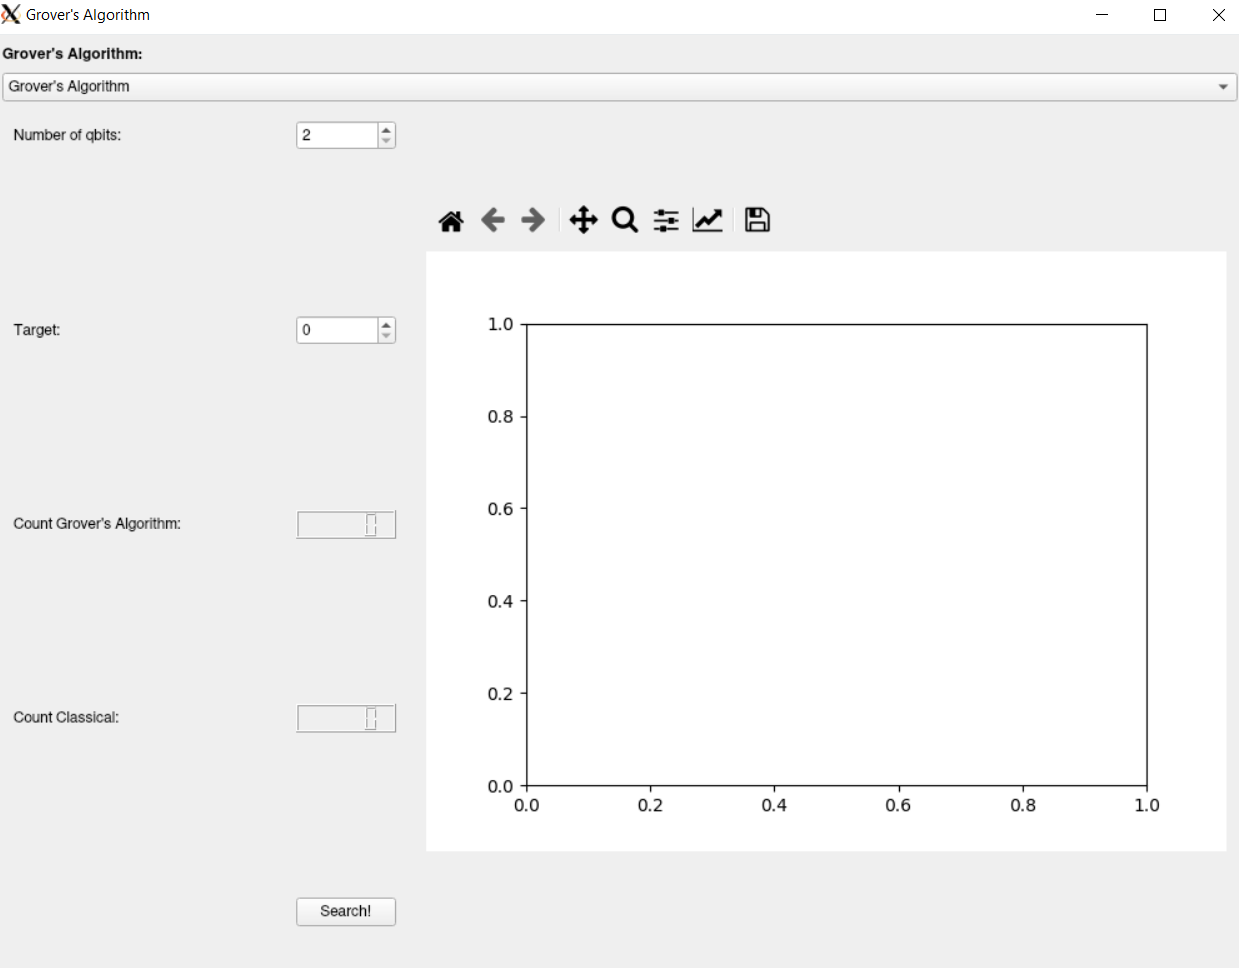
\includegraphics[width=15cm]{docs/images/gui_overview_grovers.png}
\caption{\label{fig:gui-overview-grover} Initial GUI window view}
\end{figure}

The user interface for Grover's Algorithm can be seen in Figure \ref{fig:gui-overview-grover} has two input fields.
The first field sets the number of qubits to use in the simulation.
The second is the state to target in the Grover's search, and is bounded within $0 < t < 2^{nqbits}$.

Once the input has been set, the \textit{Search} button can be clicked and the GUI will run the simulation on a separate thread. Figure \ref{fig:gui-calculation-grovers} shows an example simulation result.
Grover's Algorithm also outputs the number of iterations that the quantum simulator took to find the result, and compares it to the equivalent for a classical algorithm.

\begin{figure}[H]
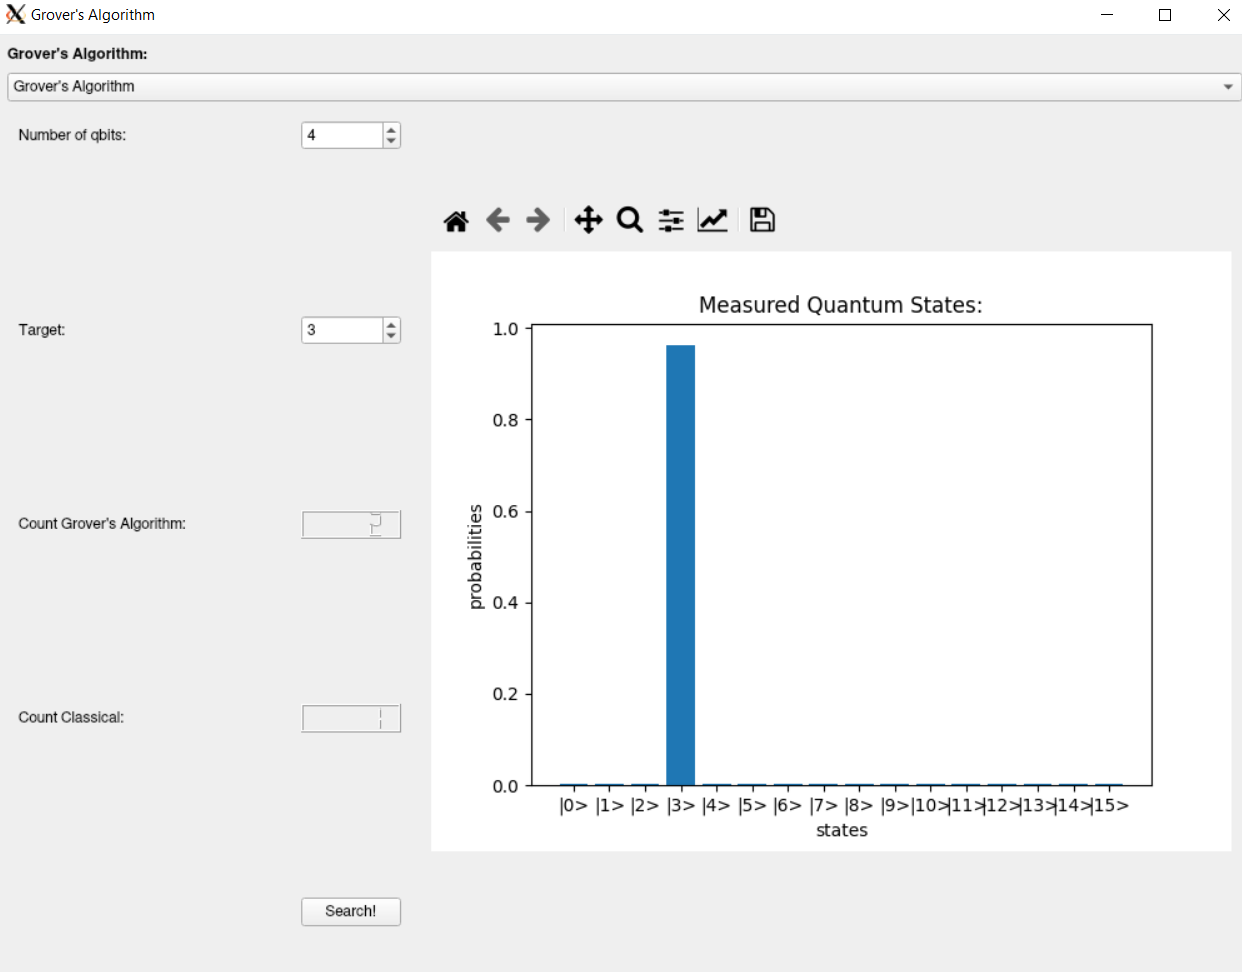
\includegraphics[width=15cm]{docs/images/gui_calculation_grovers.png}
\caption{\label{fig:gui-calculation-grovers} Sample calculation result for the Grover's Algorithm.}
\end{figure}

Once the search is completed, a plot of the probability of the quantum state 
being in the target state will be shown on the right.

\subsubsection{Phase Estimation}

\begin{figure}[H]
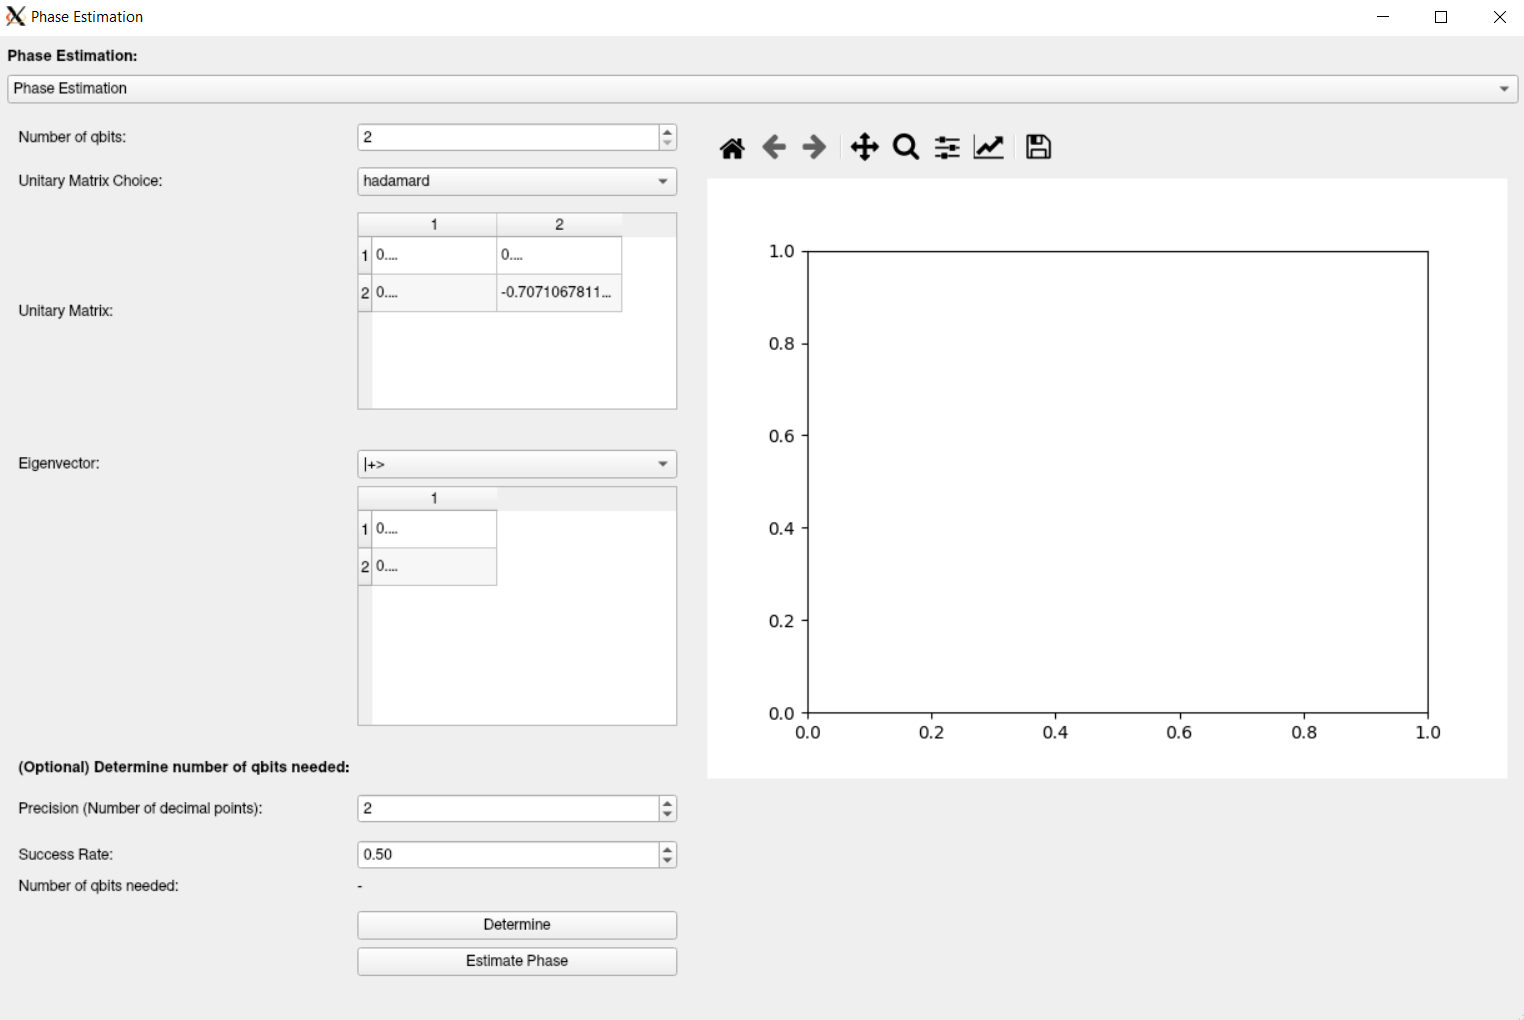
\includegraphics[width=15cm]{docs/images/gui_overview_phase_estimation.png}
\caption{\label{gui-overview-phase} Overview of the Phase Estimation GUI}
\end{figure}

The phase estimation user interface is the most complicated GUI element.
As with Grover's Algorithm, the first input field is the number of qubits to use in the simulation.
The phase estimation then requires input of two matrices, a \textit{unitary matrix}, and an \textit{eigenvector}.
To help with this input, the GUI has helper elements to select some defaults.

\medskip

For the \textit{Unitary Matrix}, a dropdown element is present that allows the user to select two pre-defined
matrices, the \verb#HADAMARD# gate, or the \verb#PHASE_SHIFT# gate.
When the drop down list is changed, the table showing the matrix is updated with the appropriate values for that Unitary Matrix.

\medskip

For the \verb#PHASE SHIFT# gate, two new GUI elements also appear, that allows the user to set the
phases in the two diagonal elements (Figure \ref{fig:gui-overview-phase-2}).

\begin{figure}[H]
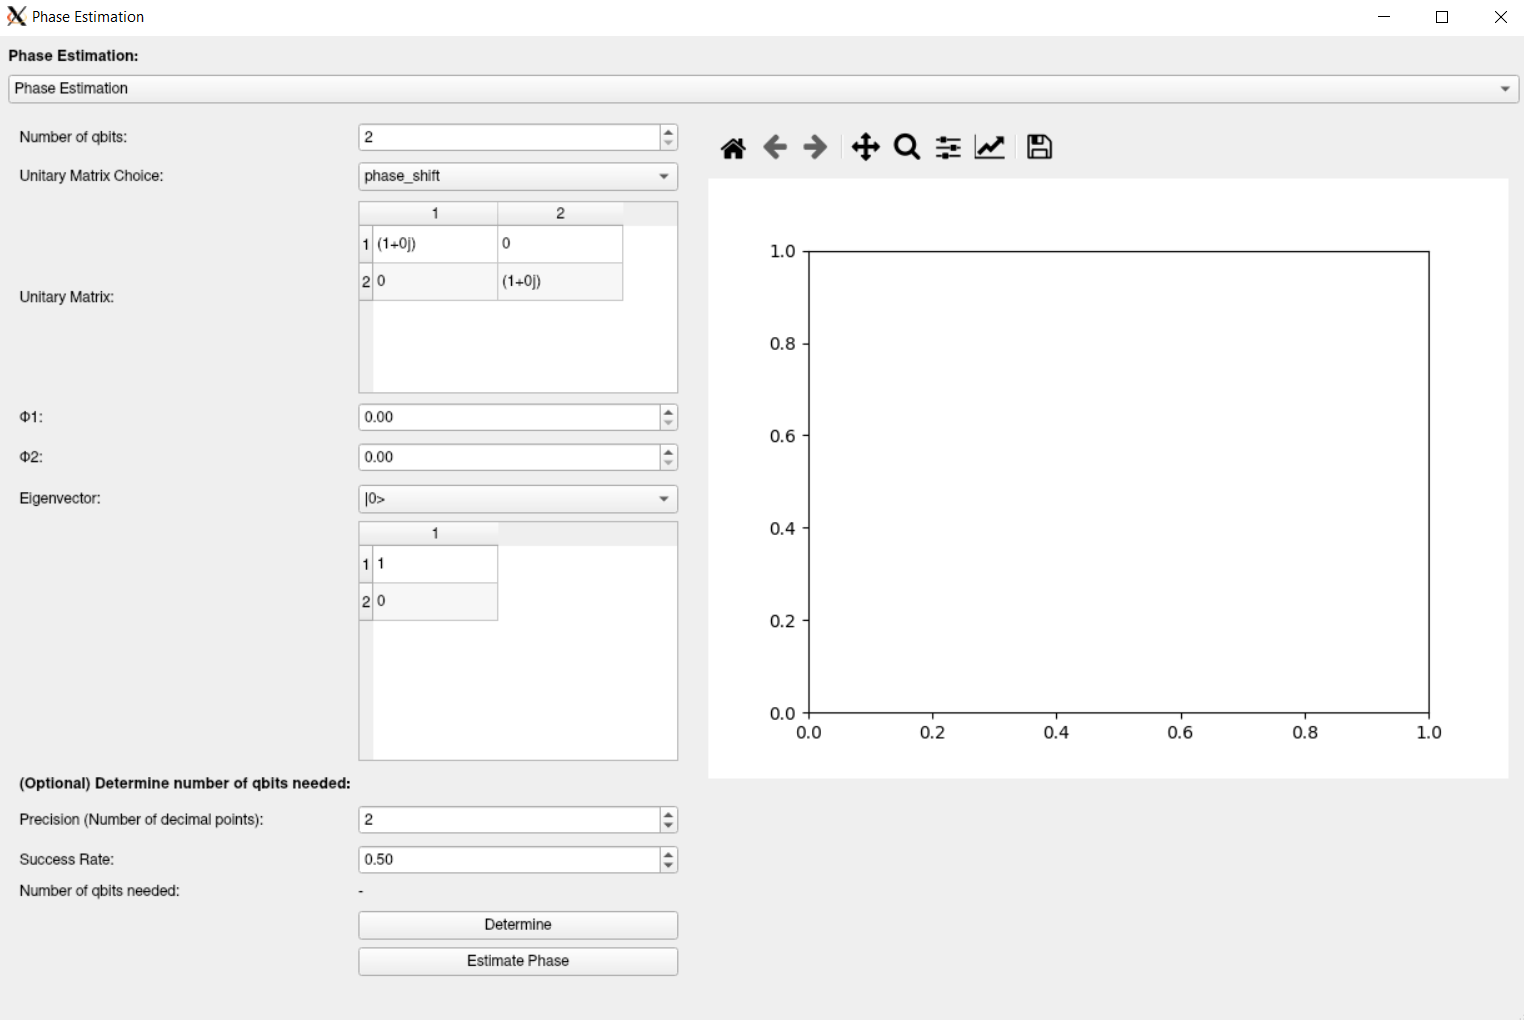
\includegraphics[width=15cm]{docs/images/gui_overview_phase_estimation_2.png}
\caption{\label{fig:gui-overview-phase-2} The phase estimation GUI showing the $\phi_1$ \& $\phi_2$ input fields.}
\end{figure}

\medskip

Once the user has selected a unitary matrix, they can then follow similar steps to select an eigenvector.
The dropdown list for the eigenvectors changes per choice of unitary matrix.

\medskip

For the \verb#HADAMARD# gate, the two choices are the bases $\ket{+}$ & $\ket{-}$.

\medskip

For the \verb#PHASE SHIFT# gate, the two choices are the bases $\ket{0}$ & $\ket{1}$.

\medskip

Of course, the user can always input custom matrices manually into the matrix fields displayed in the GUI, and the GUI will perform checks on the validity of the matrices before beginning the simulation.
Any \textit{integer}/\textit{float}/\textit{complex} numeric type is an acceptable parameter.
If there are any issues with the inputs of the two matrices once the simulation is set to start, the simulation will quit and a useful error message will appear beside the matrix at fault with a message pin-pointing the entry at fault.

\medskip

At the bottom of the UI element, there are two extra fields:
\textit{Precision} and \textit{Success Rate}, these determine the number of decimal points we want to estimate the phase to (the "precision"), and the acceptable rate that the results could be inaccurate ("success rate").
If the user wishes to get a more acceptable answer, they can input their parameters, and click the \textit{Determine} button, in which case the GUI will calculate the number of qubits to use to get this accuracy, and auto-set the number of qubits field.

\begin{figure}[H]
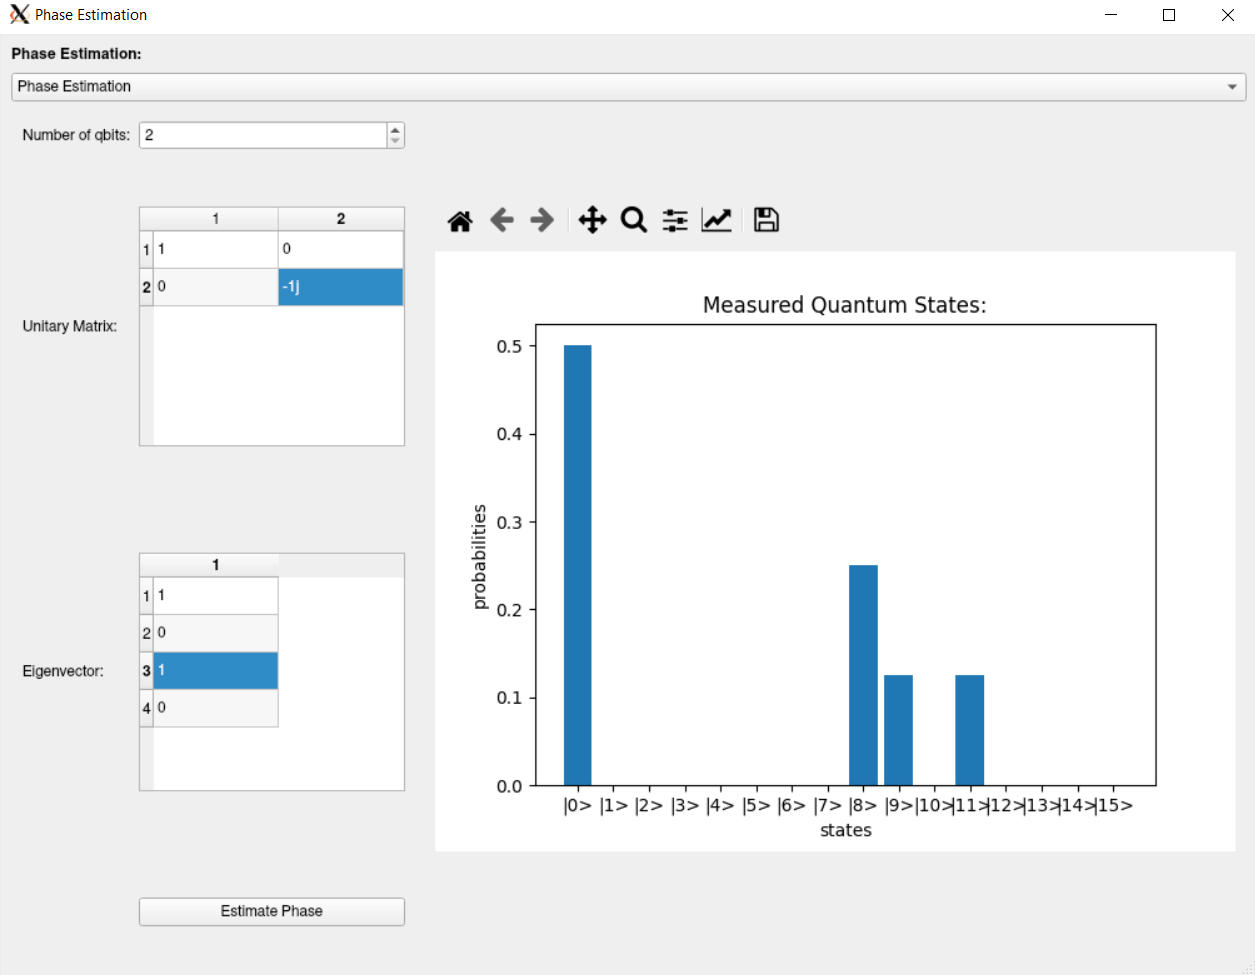
\includegraphics[width=15cm]{docs/images/gui_calculation_phase_estimation.png}
\caption{\label{gui-calculation-phase} Sample calculation result for the Phase Estimation Algorithm.}
\end{figure}

When the phase estimation result is computed, the probabilities are shown in the graph on the right for each state.

\subsubsection{Sudoku}

\begin{figure}[H]
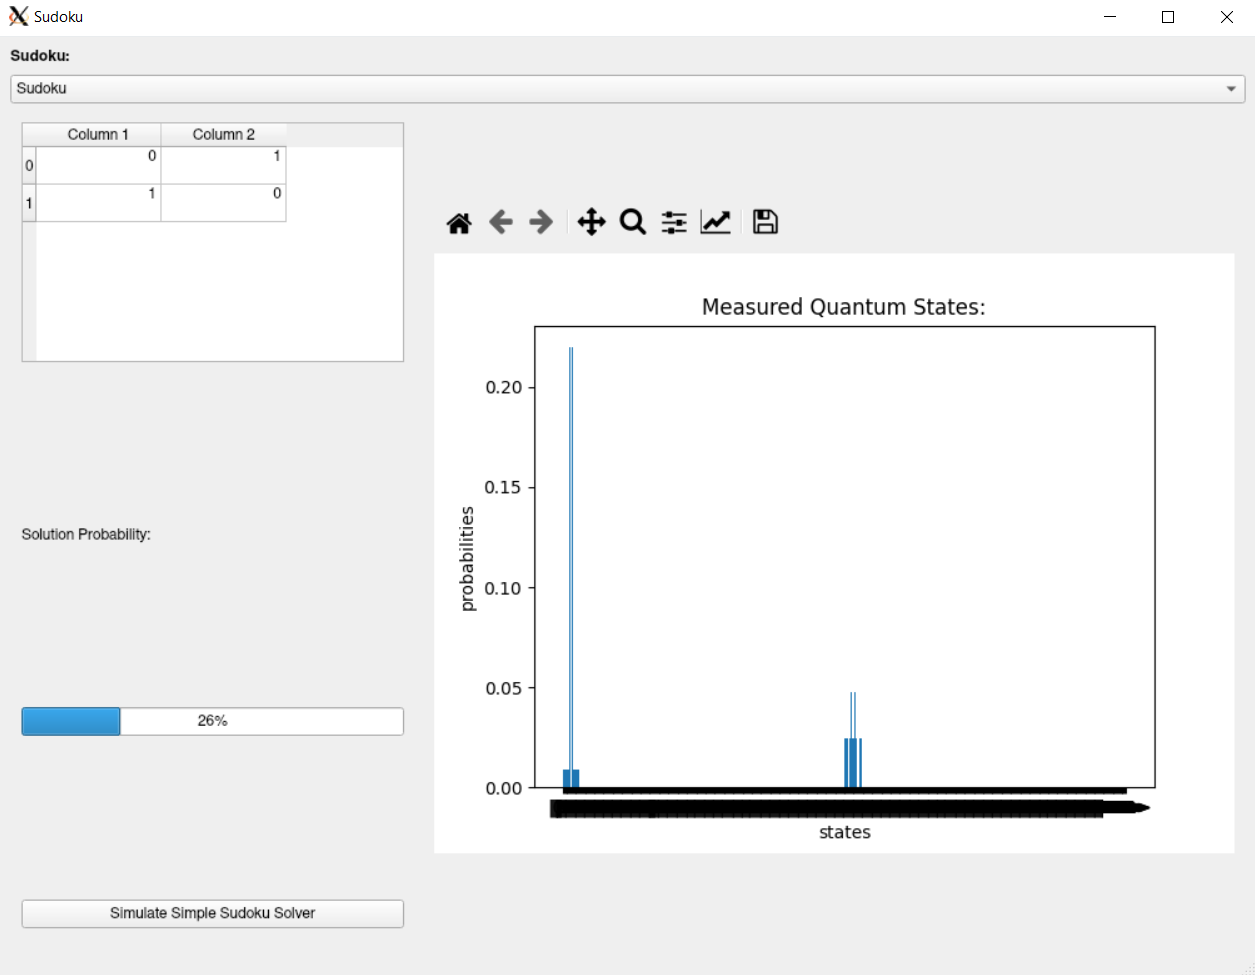
\includegraphics[width=15cm]{docs/images/gui_calculation_sudoku.png}
\caption{\label{fig:gui-calculation-sudoku} Sample calculation result for the Sudoku Algorithm.}
\end{figure}

The Sudoku algorithm takes no explicit input, so the simulation can be run straight away using the \textit{Simulate Simple Sudoku Solver} button.

\begin{figure}[H]
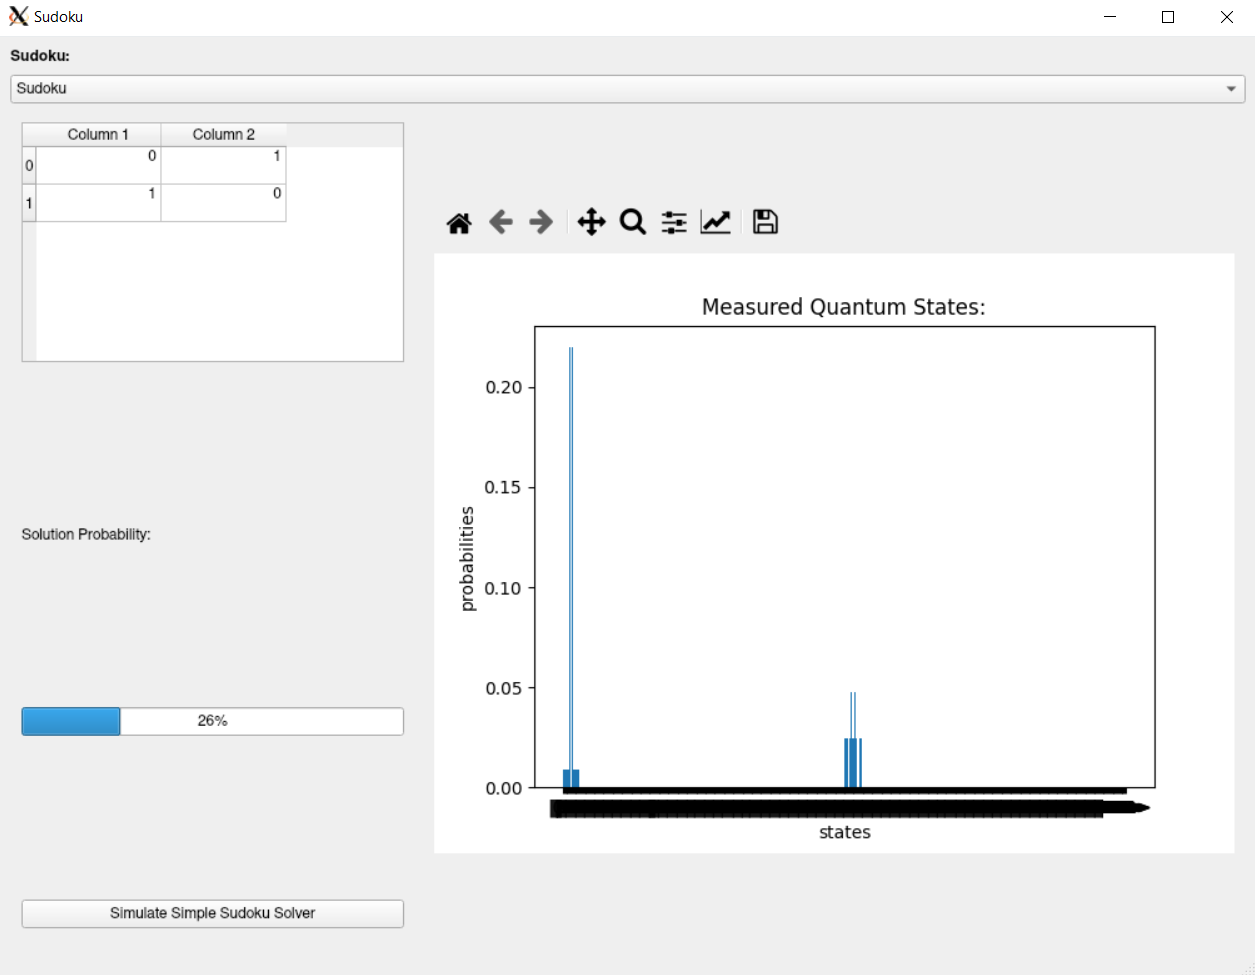
\includegraphics[width=15cm]{docs/images/gui_calculation_sudoku.png}
\caption{\label{gui-calculation-sudoku} Sample calculation result for the Sudoku solver Algorithm.}
\end{figure}

Sudoku also outputs a probability distribution in the graph on the right.
For the simple \textit{2x2} sudoku problem, a sample layout is also shown in a table, with the probability calculated by the algorithm for that state to be the accepted result.

\pagebreak

\section{Issues and Challenges}

Over the course of the project we experienced few challenges:
Some team members had little experience with quantum mechanics, programming, or tertiary tool, like GitHub, which meant that time was spent having to learn those skills beforehand.
As with solving any programming task bugs that were discovered. Meeting in person was considered ideal, However it was difficult for the team to all organise to meet together, and of course there were technical issues.
All of these challenges are not unique to our project and are an inevitability when programming in a team.
However, there were two major problems that needed immediate attention when implementing our project.

\subsection{Debugging large matrices}

A Sudoku is usually solved on a \textit{9x9} grid, to simplify the task of implementing an algorithm to solve Sudoku based on the \textit{Grover's} Algorithm, it was only possible to simulate solving a simple \textit{2x2} Sudoku problem.
However, even with this simple \textit{2x2} restriction, it still lead to an algorithm that needed 9 qubits which in turn translated to square matrices representing gates of size 512.
This makes a full Sudoku solving algorithm impossible to run on a classical computer, since even with the simple restriction of \textit{2x2} we are running close to the upper limit of the number of qubits that can be simulated on a classical laptop computer.
The rate at which new qubits are added is not linear which increases the computing power necessary even further.
This means that this algorithm is impractical on anything other than an actual quantum computer and even for smaller Sudoku puzzles it places a strain on both the user and developer. 

\subsection{Convention for applying Gates}

While syntax, run-time, and most logical errors were easily caught by the tests (section \ref{testing}) that were designed by the team, there was one logical error that was not discovered and fixed until a week before the March 23rd deadline.
By convention quantum gates are applied from right to left (little-endian notation), however the development team at the time made a mistake by implementing the logic that generates the gates using Big-endian (left to right) notation.
This flipped some of the logic gates implementation logic, and was first noticed in the Sudoku Algorithm.
This was not a technical error since the algorithm still worked correctly however it was deemed as an error since it went against the natural convention in an unintended manner.
With all that being said these bugs were fixed and they helped the team catch more errors in the future.

\pagebreak

\section{State of the Art: Quantum Computers}

\noindent
The idea of combining quantum mechanics and information theory appeared in the 1970s, but received little attention until 1981, when physicist Richard Feynman gave a presentation arguing that computation based on classical logic could not process calculations representing quantum phenomena in a tractable manner. \cite{gamble2019quantum} “Nature isn’t classical, dammit, and if you want to make a simulation of nature, you’d better make it
quantum mechanical”, the physicist Richard Feynman famously quipped. “And by golly it’s a
wonderful problem, because it doesn’t look so easy.” \cite{huang2020superconducting}
Later in 1994, quantum computing received even more attention when mathematicial Peter Shor developed a quantum algorithm. The algorithm could find the prime factors of large numbers in a time efficient manner, which was far better than the efficiency of the current state-of-the-art of classical algorithms.

\vspace{5mm}


Quantum computers can be implemented using a variety of quantum systems, such as trapped ions, superconducting qubits, photons, and silicon. Over last couple of decades, numerous advances have been attempted to try and build large scale quantum computers. Superconducting qubits, in particular, have emerged as a major possibility for such large scale quantum prcessor architecture.

\noindent
\subsection{Superconducting Quantum Computers}
\noindent
Yasunobu Nakamura, in 1999, produced the first simple qubit for superconducting computing. As a result, superconducting quantum computing has advanced significantly in recent years, with the number of qubits rapidly increasing and the quality of qubits rapidly improving. The major milestone, known as quantum supremacy, which represents a significant achievement in paving the way towards quantum computing, was first exhibited using the superconducting quantum systems in 2019. Due to this rapid development in the sector of superconducting quantum computers, the worldwide race towards the quantum computer is in full swing.\cite{huang2020superconducting}
Many companies like Honeywell, IBM, Google, and Intel are competing for having dominance in the quantum computers region. Up and coming players like IonQ and Rigetti have also stepped into the field to advance the technology. While the field is still evolving, there have been some major advancements by these companies in the fields like pharmaceutical and chemical industries, risk in the finance industry, and aid in cybersecurity across a multitude of industries, suing the power of quantum computation.   \cite{noauthor_quantum_nodate-2} 
All of these initiatives have resulted in a bright future for superconducting quantum computing. 



\vspace{5mm}

\subsection{IBM: 127 qubit eagle processor}
IBM, on November 16, 2021, announced its new 127-qubit 'Eagle' processor at the IBM Quantum Summit 2021, the annual event held by IBM to showcase their milestones in quantum hardware, software, and the growth of the quantum ecosystem. 'Eagle' is IBM's first quantum processor developed and deployed to contain more than 100 operational and connected qubits. It is preceded by IBM's 65-qubit 'Hummingbird' processor released in 2020 and the 27-qubit 'Falcon' processor released in 2019.

\noindent
The new techniques used within Eagle apply control wiring on multiple physical levels within the processor, keeping the qubits on a single layer, which enables a significant increase in qubits. \cite{noauthor_ibm_nodate}

\begin{figure}[H]
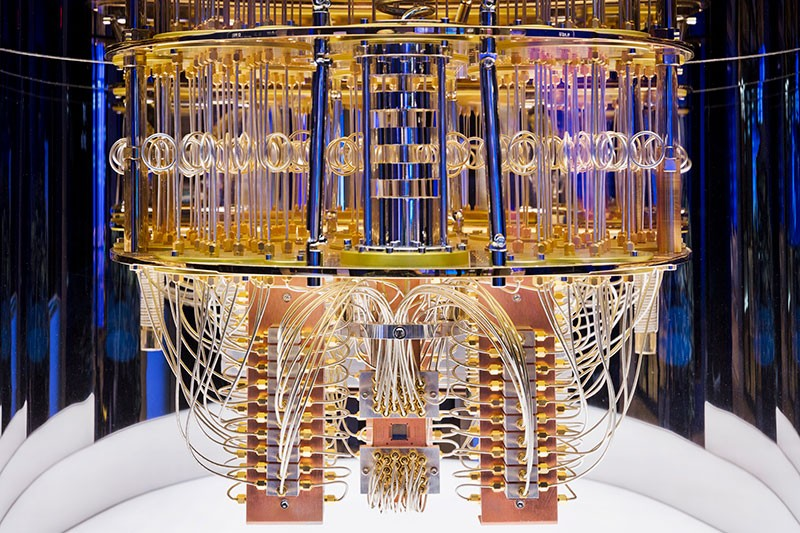
\includegraphics[width=16cm]{docs/images/IBM.jpg}
\caption{The innards of an IBM quantum computer show the tangle of cables used to control and read out its qubits. \cite{ball_first_2021}}
\end{figure}


\pagebreak

\section{Conclusion} % Numbered section

Every Friday a meeting was held once the group members were assigned. We would discuss the tasks to be completed and the corresponding team members would work on these tasks until the next Friday meeting. Any queries and disputes were discussed and resolved at these meetings. This continued until a working simulator for the project was completed. Of course, these algorithms are not faster than traditional algorithms when simulated on a classical computer and are therefore not practical to be used seriously. However, this was more of an exercise in proving that a quantum algorithm can work without actually using a quantum system. To be able to work as a team, we decided to use GitHub to share files. Getting familiar with this work environment will prove to be helpful in future projects. Team members learned programming and presentation skills from each other, which they were not experienced in prior to this project. A few members that were less experienced with programming learned from the development teams tricks to program more efficiently, while members that were not as familiar with \LaTeX{} learned from the report team. Skills that were weak in every member were strengthened thanks to this project.


\section{References and Bibliography}
\printbibliography[heading=none]

\end{document}
https://www.overleaf.com/project/621f925c52bf57288226281e